%%%%%%%%%%%%%%%%%%%%%%%%%%%%%%%%%%%%%%%%%%%%%%%%%%%%%%%%%%%%%%%
%
%     filename  = "gullifer-diss.tex",
%     version   = "1",
%     date      = "06/02/2015",
%     authors   = "Jason W. Gullifer",
%     copyright = "Jason W. Gullifer",
%     address   = "Department of Psychology
%                  7 Moore Building,
%                  Penn State University,
%                  University Park, PA 16802,
%                  USA",
%     telephone = "978.273.8062",
%     email     = "jwg20@psu.edu",
%
%%%%%%%%%%%%%%%%%%%%%%%%%%%%%%%%%%%%%%%%%%%%%%%%%%%%%%%%%%%%%%%
%
% Change History:
%
% 1.3.0	**	Added the cite package.
%
%		**	Give that the Graduate School now allows essentially
%			any line spacing, I have moved the line space setting
%			from psuthesis.cls to this driver file. Go ahead and
%			make it ugly if you want. :-)
%
%		**	Removed \addtocounter{page}{-1} after \psutitlepage is
%			executed. It made the paging of the frontmatter
%			incorrect. I can no longer remember why it was there.
%
%		**	Removed \psusigpage since the Graduate School now
%			provides the signature page.
%
%		**	Added the command \collegesubmittedto to add the College
%			in which the thesis/dissertation has been completed to
%			the title page.
%
%		**	Added instructions for documents that include a single
%			appendix since the Graduate School just hates calling it
%			``Appendix A'' is there is a single appendix.
%
%		**	Removed the fncychap package since I could not easily
%			find a way to make it work with documents that have a
%			single appendix.
%
%		**	Added the titlesec package so that the user can make the
%			format of the chapter titles a little less boring than
%			LaTeX's default.
%
% 1.2.2	**	Added some information to the main driver file (this
%			file) regarding the use of hyperref with the
%			psuthesis class. Thanks to Nathan Urban for pointing
%			out the included workaround.
%
% 1.2.1	**	Finally reproduced and fixed the problem where the
%			page number listed in the TOC for the Bibliography
%			was the last page number of the Bibliography.
%
%		**	Added 10pt and 11pt options to the document class,
%			though we have no idea why anyone would want to use
%			such insanely small font sizes since it will lead to
%			line lengths that are much too long.
%
% 1.2.0	**	Two additional class options have been added to
%			support honors theses submitted to the Schreyer
%			Honors College. These options are:
%			- honors
%			- honorsdepthead
%			See below for details.
%
%		**	We have also added the commands:
%			- honorsdegreeinfo
%			- honorsadviser
%			- honorsdepthead
%			Again, see below for details.
%
% 1.1.2	**	If you want to use the subfigure package with our
%			psuthesis class file, then you must must find the 
%			following line in the psuthesis.cls file:
%
%			\RequirePackage{tocloft}
%
%			and add the subfigure option. We have already set
%			this up for you in the psuthesis.cls file to make
%			this easy to do.
%
% 1.1.1	**	Added the fncychap package to the distribution.
%
% 1.1.0	**	The way that the thesis frontmatter and backmatter
%			is generated has been completely re-done in order
%			to be more intuitive.
%
%		**	We have added the ability to change the title of
%			the Dedication/Epigraph to anything you please.
%
%		**	In the process of changing the format of the Table
%			of Contents to conform to the inflexible rules of
%			the Grad School (the word ``Chapter'' and
%			``Appendix'' need to appear before the number and
%			letter, respectively), we have added an option to
%			the class called inlinechaptertoc that changes the
%			format of the Chapter/Appendix entries in the TOC.
%			Note that the tocloft package is now required.
%
%		**	Appendices should now start with the
%			\Appendix command rather than \chapter. See the
%			accompanying files for examples.
%
%		**	Added information regarding the Nontechnical
%			Abstract that is required of ESM students.
%
%		**	Added the fncychap package for those of you who like
%			the nice Chapter headings it provides. We like
%			Lenny, but you don't have to use it if you don't
%			want to. In addition, the other options are: Sonny,
%			Glenn, Conny, Rejne, and Bjarne
%
% 1.0.4	**	fixed the \addcontentsline entry for BibTeX within
%			the commented out text in the Bibliography section
%
% 1.0.3	**	added a sigpage option to conform to new Grad School
%			requirements
%
% 1.0.2	**	issued the \appendix command to start the appendices
%
%		**	moved the \addcontentsline for the bibliography so
%			that the bibliography now shows up on the right page
%			in the TOC
%
%		**	added some info if you use bibtex
%
% 1.0.1	**	eqlist and eqparbox are now included in the archive
%
%%%%%%%%%%%%%%%%%%%%%%%%%%%%%%%%%%%%%%%%%%%%%%%%%%%%%%%%%%%%%%%
%
% This is a template file to help get you started using the
% psuthesis.cls for theses and dissertations at Penn State
% University. You will, of course, need to put the
% psuthesis.cls file someplace that LaTeX will find it.
%
% We have set up a directory structure that we find to be clean
% and convenient. You can readjust it to suit your tastes. In
% fact, the structure used by our students is even a little
% more involved and commands are defined to point to the
% various directories.
%
% This document has been set up to be typeset using pdflatex.
% About the only thing you will need to change if typesetting
% using latex is the \DeclareGraphicsExtensions command.
%
% The psuthesis document class uses the same options as the
% book class. In addition, it requires that you have the
% ifthen, calc, setspace, and tocloft packages.
%
% The first additional option specifies the degree type. You
% can choose from:
%	Ph.D. using class option <phd>
%	M.S. using class option <ms>
%	M.Eng. using class option <meng>
%	M.A. using class option <ma>
%	B.S. using class option <bs>
%	B.A. using class option <ba>
%	Honors Baccalaureate using the option <honors>
%
% If you specify either ba or bs in addition to honors, it will
% just use the honors option and ignore the ba or bs option.
%
% The second additional option <inlinechaptertoc> determines
% the formatting of the Chapter entries in the Table of
% Contents. The default sets them as two-line entries (try it).
% If you want them as one-line entries, issue the
% inlinechaptertoc option.
%
% The class option ``honors'' should be used for theses
% submitted to the Schreyer Honors College. This option
% changes the formatting on the Title page so that the
% signatures appear on the Title page.
%
% The class option ``honorsdepthead'' adds the signature of the
% department head on the Title page for those baccalaureate
% theses that require this.
%
% The class option ``secondthesissupervisor'' should be used
% for baccalaureate honors degrees if you have a second
% Thesis Supervisor.
%
% The vita is only included with the phd option and it is
% placed at the end of the thesis. The permissions page is only
% included with the ms, meng, and ma options.
%%%%%%%%%%%%%%%%%%%%%%%%%%%%%%%%%%%%%%%%%%%%%%%%%%%%%%%%%%%%%%%
% Only one of the following lines should be used at a time.
\documentclass[phd,inlinechaptertoc,12pt]{psuthesis}
%\documentclass[draft,phd,inlinechaptertoc]{psuthesis}
%\documentclass[draft,ms]{psuthesis}
%\documentclass[draft,honorsdepthead,honors]{psuthesis}
%\documentclass[phd,12pt]{psuthesis}
%\documentclass[draft,secondthesissupervisor,honors]{psuthesis}
%\documentclass[draft,bs]{psuthesis}

\usepackage[T1]{fontenc}
\usepackage{lmodern}
\usepackage{textcomp}
\usepackage{microtype}

%%%%%%%%%%%%%%%%%%%%%%%%%%%%
% Packages we like to use. %
%%%%%%%%%%%%%%%%%%%%%%%%%%%%
\usepackage{amsmath}
\usepackage{amssymb}
%\usepackage{amsthm}
%\usepackage{exscale}
%\usepackage[mathscr]{eucal}
%\usepackage{bm}
\usepackage{eqlist} % Makes for a nice list of symbols.
\usepackage[final]{graphicx}
\usepackage[dvipsnames]{color}
\DeclareGraphicsExtensions{.pdf, .jpg}
\usepackage{pdflscape}
\usepackage{booktabs}

\usepackage{color}   %May be necessary if you want to color links


\usepackage[american]{babel}
\usepackage[style=apa, backend=biber, uniquename=false]{biblatex}

\AtEveryBibitem{
  \clearfield{labelmonth}
  \clearfield{month}
  \clearfield{url}
  \clearfield{number}
}

\usepackage{longtable}
\usepackage{tipa,csquotes,verbatim,graphicx,linguex,setspace,pdfpages}
\DeclareLanguageMapping{american}{american-apa}
%\bibliography{C:/Users/jason/Documents/library} %home use
\bibliography{/home/jason/Documents/library} %home use

% http://www.tex.ac.uk/cgi-bin/texfaq2html?label=citesort
%\usepackage{cite}

\usepackage{titlesec}



%%%%%%%%%%%%%%%%%%%%%%%%%%%%%%%
% Use of the hyperref package %
%%%%%%%%%%%%%%%%%%%%%%%%%%%%%%%
%
% This is optional and is included only for those students
% who want to use it.
%
% To the hyperref package, uncomment the following line:
\usepackage{hyperref}

\hypersetup{
    colorlinks=true, %set true if you want colored links
    linktoc=all,     %set to all if you want both sections and subsections linked
    linkcolor=black,  %choose some color if you want links to stand out
    citecolor=blue,
    urlcolor=blue
}
%
% Note that you should also uncomment the following line:
\renewcommand{\theHchapter}{\thepart.\thechapter}
%
% to work around some a problem hyperref has with the fact
% the psuthesis class has unnumbered pages after which page
% counters are reset.

% Set the baselinestretch using the setspace package.
% The LaTeX Companion claims that a \baselinestretch of
% 1.24 gives one-and-a-half line spacing, which is allowed
% by the PSU thesis office. As of October 18, 2013, the Graduate
% School states ``The text of an eTD may be single-, double- or
% one- and-a-half-spaced.'' Go nuts!
\setstretch{1.24}


%%%%%%%%%%%%%%%%%%%%%%%%%%%%%%%%%%%%
% SPECIAL SYMBOLS AND NEW COMMANDS %
%%%%%%%%%%%%%%%%%%%%%%%%%%%%%%%%%%%%
%\input{SupplementaryMaterial/UserDefinedCommands}
\newcommand{\citet}{\textcite}
\newcommand{\citep}{\parencite}

%%%%%%%%%%%%%%%%%%%%%%%%%%%%%%%%%%%%%%%%%
% Renewed Float Parameters              %
% (Makes floats fit better on the page) %
%%%%%%%%%%%%%%%%%%%%%%%%%%%%%%%%%%%%%%%%%
\renewcommand{\floatpagefraction}{0.85}
\renewcommand{\topfraction}      {0.85}
\renewcommand{\bottomfraction}   {0.85}
\renewcommand{\textfraction}     {0.15}

% ----------------------------------------------------------- %

%%%%%%%%%%%%%%%%
% FRONT-MATTER %
%%%%%%%%%%%%%%%%
% Title
\title{Using syntactic priming to identify cross-language constraints in bilingual language processing}

% Author and Department
\author{Jason William Gullifer}
\dept{Psychology and Language Science}
% the degree will be conferred on this date
\degreedate{August 2015}
% year of your copyright
\copyrightyear{2015}

% This command is used for students submitting a thesis to the
% Schreyer Honors College. The argument of this command should
% contain every after the word ``requirements'' that appears on
% the title page. This provides the needed flexibility for
% all the degree types.
%\honorsdegreeinfo{for a baccalaureate degree \\ in Engineering Science \\ with honors in Engineering Science}

% This is the document type. For example, this could also be:
%	Comprehensive Document
%	Thesis Proposal
%\documenttype{Thesis}
\documenttype{Dissertation}
%\documenttype{Comprehensive Document}


% This will generally be The Graduate School, though you can
% put anything in here to suit your needs.
\submittedto{The Graduate School}

% This is the college to in which you are submitting the
% thesis/dissertation.
\collegesubmittedto{College of the Liberal Arts}


%%%%%%%%%%%%%%%%%%
% Signatory Page %
%%%%%%%%%%%%%%%%%%
% You can have up to 7 committee members, i.e., one advisor
% and up to 6 readers.
%
% Begin by specifying the number of readers.
\numberofreaders{5}

% For baccalaureate honors degrees, enter the name of your
% honors adviser below.
%\honorsadviser{Honors P. Adviser}

% For baccalaureate honors degrees, if you have a second
% Thesis Supervisor, enter his or her name below.
%\secondthesissupervisor{Second T. Supervisor}

% For baccalaureate honors degrees, certain departments
% (e.g., Engineering Science and Mechanics) require the
% signature of the department head. In that case, enter the
% name of your department head below.
%\honorsdepthead{Department Q. Head}

% Input reader information below. The optional argument, which
% comes first, goes on the second line before the name.
\advisor[Dissertation Co-Advisor]
        {Judith F. Kroll\\ Chair of Committee}        
        {Distinguished Professor of Psychology, Linguistics, and Women's Studies\\
        Director, Center for Language Science}

\readerone[Dissertation Co-Advisor]
          {Paola E. Dussias}
          {Professor of Spanish, Linguistics, and Psychology\\
          Associate Director, Center for Language Science}

\readertwo[]
           {Carol Miller}
           {Associate Professor of Communication Sciences and Disorders}

\readerthree[]
          {Janet Van Hell}
          {Professor Psychology and Linguistics\\
           Director, Linguistics Program}

\readerfour[]
            {Brad Wyble}
            {Assistant Professor of Psychology}

\readerfive[Department Head]
           {Melvin M. Mark}
           {Professor of Psychology}


% Format the Chapter headings using the titlesec package.
% You can format section headings and the like here too.
\definecolor{gray75}{gray}{0.75}
\newcommand{\hsp}{\hspace{15pt}}
\titleformat{\chapter}[display]{\fontsize{30}{30}\selectfont\bfseries\sffamily}{Chapter \thechapter\hsp\textcolor{gray75}{\raisebox{3pt}{|}}}{0pt}{}{}

\titleformat{\section}[block]{\Large\bfseries\sffamily}{\thesection}{12pt}{}{}
\titleformat{\subsection}[block]{\large\bfseries\sffamily}{\thesubsection}{12pt}{}{}


% Makes use of LaTeX's include facility. Add as many chapters
% and appendices as you like.
\includeonly{%
maintext.tex/maintext%
}

\usepackage{listings}
%%%%%%%%%%%%%%%%%
% THE BEGINNING %
%%%%%%%%%%%%%%%%%
\begin{document}
%%%%%%%%%%%%%%%%%%%%%%%%
% Preliminary Material %
%%%%%%%%%%%%%%%%%%%%%%%%
% This command is needed to properly set up the frontmatter.
\frontmatter

%%%%%%%%%%%%%%%%%%%%%%%%%%%%%%%%%%%%%%%%%%%%%%%%%%%%%%%%%%%%%%
% IMPORTANT
%
% The following commands allow you to include all the
% frontmatter in your thesis. If you don't need one or more of
% these items, you can comment it out. Most of these items are
% actually required by the Grad School -- see the Thesis Guide
% for details regarding what is and what is not required for
% your particular degree.
%%%%%%%%%%%%%%%%%%%%%%%%%%%%%%%%%%%%%%%%%%%%%%%%%%%%%%%%%%%%%%
% !!! DO NOT CHANGE THE SEQUENCE OF THESE ITEMS !!!
%%%%%%%%%%%%%%%%%%%%%%%%%%%%%%%%%%%%%%%%%%%%%%%%%%%%%%%%%%%%%%

% Generates the title page based on info you have provided
% above.
\psutitlepage

% Generates the committee page -- this is bound with your
% thesis. If this is an baccalaureate honors thesis, then
% comment out this line.
\psucommitteepage

% Generates the abstract. The argument should point to the
% file containing your abstract. 
\thesisabstract{SupplementaryMaterial/Abstract}

% Generates the Table of Contents
\thesistableofcontents

% Generates the List of Figures
\thesislistoffigures

% Generates the List of Tables
\thesislistoftables

% Generates the List of Symbols. The argument should point to
% the file containing your List of Symbols. 
%\thesislistofsymbols{SupplementaryMaterial/ListOfSymbols}

% Generates the Acknowledgments. The argument should point to
% the file containing your Acknowledgments. 
\thesisacknowledgments{SupplementaryMaterial/Acknowledgments}

% Generates the Epigraph/Dedication. The first argument should
% point to the file containing your Epigraph/Dedication and
% the second argument should be the title of this page. 
%\thesisdedication{SupplementaryMaterial/Dedication}{Dedication}



%%%%%%%%%%%%%%%%%%%%%%%%%%%%%%%%%%%%%%%%%%%%%%%%%%%%%%
% This command is needed to get the main part of the %
% document going.                                    %
%%%%%%%%%%%%%%%%%%%%%%%%%%%%%%%%%%%%%%%%%%%%%%%%%%%%%%
\thesismainmatter

%%%%%%%%%%%%%%%%%%%%%%%%%%%%%%%%%%%%%%%%%%%%%%%%%%
% This is an AMS-LaTeX command to allow breaking %
% of displayed equations across pages. Note the  %
% closing the "}" just before the bibliography.  %
%%%%%%%%%%%%%%%%%%%%%%%%%%%%%%%%%%%%%%%%%%%%%%%%%%
\allowdisplaybreaks{
%\pagestyle{fancy}
%\fancyhead{}
%
%%%%%%%%%%%%%%%%%%%%%%
% THE ACTUAL CONTENT %
%%%%%%%%%%%%%%%%%%%%%%
% Chapters
\chapter{Introduction} 
\label{generalintroduction}

Bilinguals who are highly proficient in both languages seem to be able to operate in one of their languages independently without influence from other languages. With the exception of perhaps a slight accent or subtle differences in wording, the speech of a highly proficient bilingual may be indistinguishable from that of a monolingual speaker. All language users, monolingual, bilingual, multilingual, occasionally make speech errors, mixing up the order of words in a sentence, for example. Bilinguals however, very rarely slip up and use a word in the wrong language for the situation ~\citep{Poulisse1994}. These observations could be taken as evidence that bilinguals can functionally separate their two languages, perhaps representing the two languages in independent stores\footnote{Throughout the text, I refer to syntactic stores. I use the word stores for convenience without necessarily invoking a modular mechanism of mental representation. Instead, here, stores could just as well be represented as an emergent feature of a neural network. Shared stores would represent mostly overlapping patterns of activation, and independent stores would represent mostly differential patterns of activation.}. Indeed, the narrative in the literature on child bilingual language acquisition is that children begin life with a merged language system and eventually learn to separate the two languages ~\citep[e.g.,][]{Burns2007}, and some early brain imaging evidence suggests that the languages may be represented in distinct areas ~\citep[e.g.,][]{Kim1997}. However, psycholinguistic research on adult bilinguals who are fluent in two languages has shown that the two languages constantly interact. When a bilingual reads a word in one language, related features are co-activated in the unintended language ~\citep[e.g.,][]{Dijkstra2005}, and when a bilingual prepares to speak a word, the other language translation equivalent is on the tip of their tongue ~\citep[e.g.,][]{Kroll2006}. As such, models of the bilingual lexicon that have been proposed in the past decade posit integrated representational stores for the two languages ~\citep{Dijkstra2002}. More recent evidence from brain imaging confirms this assumption, showing that bilinguals recruit largely shared neural structure, and that when there is differential activation it reflects a differential demand on control resources ~\citep{Abutalebi2007}. Likewise in the domain of syntax, bilinguals can be primed to use a syntactic structure even if that structure was heard in a different language. This suggests that syntax is also shared across languages and on some level becomes co-activated ~\citep{Loebell2003}. Models of bilingual syntactic representation also posit shared storage of syntactic structures ~\citep{Schoonbaert2007}. Yet, the question remains: if the two languages are co-activated and interact, how does a bilingual or multilingual finally select a word or structure in the intended language from the myriad of co-activated alternatives? 

This dissertation addresses the question of how bilinguals select the language they intend to use at the lexical level and at the syntactic level. The hypothesis explored here is that features of a sentence that are distinct to one language (specifically, when syntactic constructions differ across the two language) allow bilinguals to functionally separate syntactic structures and predict the language of upcoming words in a sentence. This question is addressed through the novel combination of two distinct research paradigms: the confederate picture description task and the Rapid Serial Visual Presentation reading paradigm. The confederate picture description task measures cross-language priming (i.e., the propensity to repeat a syntactic construction, such as the active construction or the passive construction, that was used recently), providing an index of the functional separability of various syntactic constructions within a population of bilinguals. When structures are primed across languages, they are assumed to be represented in a common, language-general store. If they are not primed, they are assumed to be represented in a distinct, language-specific store. The results of previous confederate picture description studies conducted on bilinguals who speak a variety of language pairs indicate that structures which share word order across the two languages are represented in language-general stores and structures that do not share word order are represented in language-specific stores ~\citep[e.g.,][]{Bernolet2007,Loebell2003}. 

In Experiments 1 and 2 of this dissertation, the implications of these findings are applied to the domain of word recognition during reading. Experiment 1 investigates bilingual word recognition in isolation. Spanish monolinguals and Spanish-English bilinguals read aloud words that were cognates or homographs between Spanish and English. If bilinguals co-activate the unintended language, then we should observe effects that are consistent with cross-language activation (i.e., cognate facilitation and homograph inhibition) for bilinguals but not monolinguals. In Experiment 2, two sets of sentences are constructed: (1) a set of sentences with syntactic structures that are inferred to be language-specific for Spanish-English bilinguals and (2) a set of sentences with syntactic structures that are inferred to be language-general for Spanish-English bilinguals. If bilinguals co-activate the unintended language during sentence reading, then the cognate and homograph effects should persist in the sentential conditions. However, if sentence context, or aspects of sentence context such as language-specific syntactic constructions, can trigger language-selective access, then the effects should be reduced in following these conditions. In Experiment 3, a confederate picture description study is conducted on a similar sample of Spanish-English bilinguals, providing independent evidence on whether the inferences of separate vs. shared syntax hold for this set of bilingual speakers. 

To preview the findings, Experiment 1 shows that Spanish-English bilinguals activate the unintended language (here English, the L2) when they read words aloud in the L1. Co-activation was evidenced by significant facilitation for cognates relative to control words, but there was no homograph effect. In Experiment 2, the cognate facilitation and homograph inhibition effects were present but modulated by sentence construction. The cognate facilitation effect differed when comparing the two constructions in which there are hypothesized to be differences between Spanish and English: the dative conditions. Cognate facilitation was greater in the dative condition that shares word order with the English dative compared to the dative condition that does not share word order, but a follow-up analysis in which we analyzed only the subset of items that most strongly showed a cross-language effect out-of-sentence-context calls the stability of this interaction into question. The homograph effect also depended on syntactic construction: there was a facilitatory homograph effect in sentences with active and passive constructions, which share word order between Spanish and English, and an inhibitory effect in the dative constructions. The interaction was robust after the follow-up analysis. Finally, the results of Experiment 3, while preliminary, suggest that only sentences in the active and passive condition were able to be primed from Spanish to English. The dative structures, which differ in word order, showed no significant effect of priming. This suggests that for our sample of bilinguals, active and passive structures are represented in mental stores that are shared across language and that dative structures are represented in separate mental stores. This is the first demonstration, to our knowledge, of (1) a language-specific storage for syntactic structures in Spanish-English bilinguals and (2) that language-specific storage has consequences for the co-activation of the two languages during word recognition. 

The dissertation is organized out as follows. In what remains of Chapter 1, I provide an overview of the evidence for parallel activation of two languages in bilinguals, focusing on the lexical level. I then discuss the extant research constraints to language co-activation, including whether aspects of sentence context affect co-activation. In Chapter 2, I provide an theoretical and methodical road-map to the four empirical investigations in Chapters 3, 4 and 5. Specifically, I review the literature on cross-language syntactic priming and argue that data from language usage can provide valuable insights into how syntactic structure is stored representationally. In Chapter 3, two experiments are reported to provide independent evidence for lexical co-activation during word naming, in which bilinguals name words outside of sentence context. In Chapter 4, I present the empirical results of an experiment in which I investigate whether syntactic constructions that are implicated as language-specific structures by previous syntactic priming research can reduce co-activation of the unintended language at the lexical level. In Chapter 5, I report the empirical results of a cross-language syntactic priming experiment in which I investigate whether word order differences allow bilinguals to establish structures as language-specific. Finally in Chapter 6, I present the general discussion and conclusions, tying together the results of the four empirical studies. 

\section{Parallel activation at the lexical level}
\label{parallelactivationatthelexicallevel}

The strongest evidence for parallel activation of the two languages has been shown when bilinguals read single words that are ambiguous across their two languages, such as interlingual cognates and homographs. Cognates are words which share form and meaning across languages (e.g., ``piano'' in English and Spanish) while homographs overlap in form but conflict in meaning across languages (e.g., ``pan''' which is a receptacle for cooking in English but a leavened food item in Spanish). If it were possible for a bilingual to access words selectively in a single language, then the presence of cross-language ambiguity should not influence processing in comparison to non-ambiguous words. However, contrary to this prediction, cognates typically elicit faster reaction times to read or name the word ~\citep[i.e., cognate facilitation; e.g.,][]{Dijkstra1998,Schwartz2007,VanHell2002}. Inter-lingual homographs typically elicit slower processing times ~\citep[i.e., homograph inhibition; e.g., ][]{Beauvillain1987a,Dijkstra1998}. Critically, monolinguals of either language in the bilingual language pair do not show differential effects towards interlingual cognates or homographs, suggesting that the effects witnessed in bilingual participants are due to their bilingualism and not to spurious effects related to uncontrolled properties of the stimuli. In the past decade, cross-language co-activation has become a widely-accepted phenomenon in the field of bilingualism. 

Evidence for language co-activation (or language non-selectivity) is observed across a broad range of tasks and contexts. Cognate facilitation and homograph inhibition are observed using a variety of dependent measures. Initial research was conducted with behavioral measures such as reaction time for lexical decision ~\citep{Dijkstra1998, VanHell2008, VanHell2002}, translation ~\citep{VanHell2008, Sachez-Casas1992}, word association ~\citep{VanHell2002}, and word naming ~\citep{Schwartz2006, Schwartz2007}. More recent studies find language co-activation in measures such as eye-tracking ~\citep{Duyck2007, Libben2009, Titone2011, VanAssche2010,VanAssche2009} and event-related potentials ~\citep[ERPs;][]{Midgley2011}. Behavioral measures tend to measure the aggregate result of processing. Hence a cognate effect in a lexical decision task provides no information about the point in the time-course of processing at which both languages started to become activated. It could theoretically be the case that parallel activation occurs late in the process of word recognition, almost as if bilinguals translate words between their two languages, or both languages might become activated initially at the point at which orthography begins to be decoded. While there is evidence for late translation ~\citep[e.g.,][]{Thierry2007}, methods with a sensitive time-course, such as ERPs and eye-tracking, indicate that parallel activation is not solely a late process. Both language alternatives become activated early in processing and remain activated during late stages of processing. For example, in eye tracking, cognate effects are observable in first fixation duration and gaze duration measures, assumed to reflect initial lexical access. They also show that both languages remain activated throughout the time-course of processing ~\citep{Duyck2007, Libben2009, Titone2011, VanAssche2010,VanAssche2009} via cross-language effects in total reading time, a finding which could suggest that the intended language may never actually be selected categorically or that the selection is not observable without an even more sensitive measure. Non-selective access has been observed for language pairs such as Dutch and English, which share the same writing system ~\citep[e.g.,][]{Duyck2007}, in Chinese and English, which do not ~\citep[e.g.,][]{Thierry2007}, and in English and American Sign Language ~\citep[e.g.,][]{Morford2011}, one spoken and one signed language. Parallel activation is also not simply a side-effect of L2 processing. While the first or dominant language (L1) does strongly influence processing of the weaker L2, a bilingual's L2 or even L3 can become activated during L1 processing ~\citep[e.g.,][]{VanAssche2009, VanHell2002}. Overall, the degree of cross-language activation is relatively insensitive to the demands of the task at hand. Parallel activation is observed in blocked and mixed language contexts ~\citep[e.g.,][]{Gullifer2013}, indicating that the requirement to speak a single language or to juggle multiple languages does not influence the relative co-activation of the two languages.

Parallel activation is a graded phenomenon, not an all-or-nothing process. As in monolingual word recognition ~\citep{Seidenberg1989}, the activation of any particular word for a bilingual is a continuous function of a distributed pattern of activation across multiple levels of mental representations, including the orthography, phonology, and semantics. Thus, the degree of cross-language overlap at each level factors in to the degree of observable cross-language co-activation. Cognate and homograph effects are larger when words share orthographic overlap or phonological overlap across the two languages. These effects are not categorical but continuous, such that greater overlap corresponds to a larger magnitude of cross-language co-activation ~\citep[e.g.,][]{Duyck2007,Schwartz2007, VanAssche2010, VanAssche2009}. Parallel activation of the semantics is evident in homograph recognition; the conflict in meaning across the two readings of an interlingual homograph produces a cost to processing. The magnitude of cognate facilitation is impacted by the degree of semantic overlap across the two languages, but this primarily occurs through the modulation of the non-cognate reaction time ~\citep{Garcia-Albea1998}. However, cognate effects in translation have been shown to depend upon semantic factors such as word concreteness ~\citep[e.g.,][]{VanHell2008}. In sum, bilingual word recognition is an interactive process dependent on graded activation among multiple levels of representation. 

The main focus of work on parallel activation has been on the processing of cognates and homographs. However, there are at least two critiques to this approach. First, one can argue that the processing differences observed for words with cross-language overlap are simply the result of increased frequency of usage of word. For example, a Spanish-English bilingual will experience the cognate word ``bus'' twice as often as her monolingual counterpart, and this increased experience may lead to a processing advantage for that word in the bilingual's lexicon ~\citep[see e.g. the weaker-links or frequency lag hypotheses,][]{Gollan2008, Gollan2011a}. Second, it is not clear from the study of cognate and homograph processing alone that non-selective access extends to processing of every word in the lexicon. While it is likely true that increased frequency of usage is partially responsible for the cognate and homograph effects, it does not completely rule out parallel activation of languages. Cognate and homograph effects depend on the degree of orthographic overlap ~\citep[e.g., which can be calculated via the Van Orden or Levenshtein distance methods,][]{Levenshtein1966, VanOrden1987} and phonological overlap (that can be elicited from participants making auditory judgments on sound overlap) of a word between the two. Smaller cross-language effects are observed for language-ambiguous words with a less orthographic or phonological overlap, and this relationship is linear ~\citep[e.g.,][]{Dijkstra1999, Schwartz2007, VanAssche2010}. A purely frequency-dependent hypothesis would not predict sensitivity to cross-language overlap within language-ambiguous words. Touching on the second critique, further evidence in favor of the parallel activation hypothesis is the observation of cross-language effects for stimuli that share no overt similarities between the two languages and in tasks that require no overt language processing ~\citep{Chabalpress, Morford2011, Thierry2007, Wu2013}. For example when proficient Chinese-English bilinguals and monolingual speaker of each language make semantic relatedness judgments on English words, both groups of speakers show semantic priming via a positive modulation of the N400 component for related words. However, only bilinguals show an additional modulation when the Chinese translation of the English words share characters and phonology, features that were never overtly present in the experiment ~\citep{Thierry2007, Wu2010}. Likewise, deaf signers who read English activate the sign translation equivalents despite the fact that there is no phonological nor orthographic overlap between the two linguistic systems ~\citep{Morford2011}. Thus there is strong evidence for cross-language activation in spite of the frequency dependence and when stimuli other than cognates and homographs are used in experiments. 

\section{Models of bilingual word recognition}
\label{modelsofbilingualwordrecognition}

 \citet{Dijkstra2002} proposed the BIA+ model to account for parallel language activation during bilingual word recognition ~\citep[see also][]{Dijkstra1998a} for an earlier version of the BIA+ model). The BIA+ model, adapted from the Interactive Activation Model ~\citep[see][]{McClelland1981}, was designed to account for data from reading experiments conducted with bilingual participants. The model, shown in Figure \ref{fig:biaplus}, is divided into two separate levels: the task schema and the word identification system. The word identification system is responsible for handling only linguistic input while the task schema handles the demands of non-linguistic contexts. 

\begin{figure}[htbp]
\centering
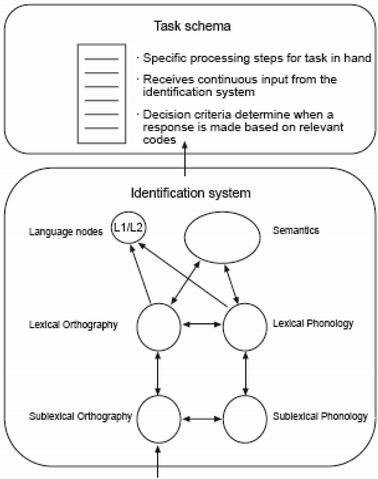
\includegraphics[width=233pt,height=296pt]{biaplus.png}
\caption{Illustration of the BIA+ model of word recognition \citep{Dijkstra2002}.}
\label{fig:biaplus}
\end{figure}

 
The word identification system deals with linguistic input to the model. The BIA+ posits an integrated lexicon (i.e., the words of each language are integrated into one ``dictionary'') and shared semantics across the two languages. The word identification system is highly interactive. Upon ``reading'' a word, nodes for phonological and orthographic representations at the lexical and sublexical levels become active. Activation then spreads within and between the lexical and sublexical levels causing potential candidates to become more highly activated than other words. The higher levels of the model (i.e., the semantics level and language nodes) receive activation from the lower levels. In the semantic level, concepts receiving enough activation spread this activation back down to the lower levels further reinforcing the activation of potential lexical candidates. The language nodes are responsible for identification of the language being read. A crucial assumption made by the model is that the higher level nodes may only receive bottom-up activation. Furthermore, the language nodes may not send activation back down to the lower levels. Thus, prior knowledge of the intended language will not increase activation to nodes at lower levels. That is, the language nodes cannot function as a language filter. Instead, the nodes must be sufficiently activated through experience with a linguistic input.

While the word identification system handles linguistic input, the task schema deals with non-linguistic contexts. The task schema is responsible for accomplishing the task at hand (e.g., lexical decision, naming, etc.) and determining when a response should be made. In order to help with this decision, this level of the model receives constant input from the word identification system. A critical assumption of the BIA+ model is that the task schema (and, thus, non-linguistic context) does not infiltrate the word recognition system. Evidence for this was shown by  \citet{Dijkstra2000} who demonstrated that the presence of stimuli and not expectations derived from instructions affected bilingual performance in a lexical decision task.

Given the assumptions of the BIA+ model it is easy to see how cross-language overlap will affect the recognition of words. Cognates, because of their close overlap in orthography, phonology, and meaning, will receive activation in both languages more quickly compared to words without similar overlap. Thus lexical decision or naming will be facilitated. On the other hand, when homographs are the input, the cross-language overlap with orthography and phonology may initially speed activation but the discrepancy in meaning will cause the system to have trouble identifying the language of the word thus slowing lexical decision or naming performance. Overall, the BIA+ predicts that a parallel access account with respect to language occurs in a bottom-up fashion. This parallel activity is not easily constrained by non-linguistic contexts. 

The question now is how linguistic contexts influence word recognition. Because the BIA+ model was designed to account for word recognition outside of sentence contexts, it makes no explicit predictions regarding linguistic contexts. However, as we shall see in the following section, there are specific linguistic contexts that may allow bilinguals to recognize words in a language-selective manner.

\section{Constraints on language co-activation}
\label{constraintsonlanguageco-activation}

A major question in multilingual word recognition is whether a single language alternative can be selected from the myriad of activated words, and if so, what cues may aid in enabling a language selection. The recent research shows that language-selective access is difficult to achieve. Neither aspects of lexical form nor of the context of language usage provide a strong language cue that can reduce co-activation of the unintended language during bilingual word recognition. 

\subsection{Aspects of lexical form}
\label{aspectsoflexicalform}

One potential source for a language cue may be present in the cross-linguistic differences between two language pairs; languages often differ on many facets. Language specific characteristics can be quantified on many different levels of representation: phonological, orthographic, morphosyntactic, syntactic, pragmatic, etc. For example, languages may differ in their phonemic inventory and phonemes that are perceived as different in one language (e.g., \slash l\slash  and \slash r\slash  in English) may be realized as the same in another language where they do not differentiate meaning (e.g., \slash l\slash  and \slash r\slash  in Japanese). Languages exhibit different phonotactic properties where for example consonant clusters may be allowed in onset position for some languages (e.g., English but not Spanish allows for complex \slash s\slash  clusters word initially, e.g., ``sprite'' is licit in English but becomes ``esprite'' in Spanish to break the cluster). Languages can have different completely different orthographic systems (e.g., contrast between the Latin, Cyrillic, and Arabic scripts of English, Russian, and Arabic), or they may contain different characters and diacritics even if most of the orthography is shared. Morphosyntactically, some languages exhibit characteristics not seen in other languages. For example, many romance languages such as Spanish have a robust system of pronominal object clitics (or proclitics, e.g., \textbf{Le} di un regalo a mi madre [I gave my mother a gift]) that does not exist in modern Germanic languages such as English or German. 

Overall, despite numerous potential differences that words can have in lexical form across the two languages for bilingual speakers, lexical form overlap is not a necessary condition for the observation of parallel activation. Cognates and homographs often exhibit slight differences in their orthographic or phonological realization between two languages; despite their overall shared form, they often have distinct phonology in each language (e.g., the cognates base and base in English and Spanish have stress on different syllables) and can also lack perfect orthographic overlap (e.g., the cognates ship and schip in English and Dutch). While the degree orthographic and phonological overlap can reduce the magnitude of cross-language effects, they do not eliminate it altogether ~\citep[e.g.,][]{VanAssche2010}. In the most extreme case, when one of the two languages in a pair lacks a system of writing entirely (such as is the case for ASL-English bilinguals) there is still significant cross-language activation. For example,  \citet{Morford2011} found that ASL-English bilinguals were facilitated in judging that two English words were semantically related if the two words also shared similar hand-shape (i.e., phonological) forms in ASL, suggesting that ASL became activated during the processing of English words, a context where ASL was not perceptually relevant. Along the same lines, the cognate facilitation effect has been demonstrated for Japanese-English bilinguals, indicating that orthographic overlap is not a necessary condition for the observation of cross-language activation ~\citep{Hoshino2008,Voga2007}. 

One aspect of lexical form that appear to function as a potential language cue is grammatical word class.  \citet{Sunderman2006} found that lexical form interference could be eliminated in a translation recognition task (i.e., decide whether two words are translations of one another) when the two words differed in their grammatical class. Likewise,  \citet{Baten2010} demonstrated that word class interacted with the degree of language co-activation for words embedded in a sentence context. A facilitatory homograph effect was present when participants were required to make a lexical decision to target words, but only when the meaning of the homograph shared grammatical class with its translation. For example, when the Dutch-English homograph brief was used as an adjective in an English sentence (brief is a noun meaning letter in Dutch) no homograph interference was observed, suggesting that higher order grammatical properties such as word class can provide information that that can aid bilinguals in selecting the target language. In each of these examples, it is not clear whether the locus of selection occurs early or late in processing. Although more evidence overall suggests a late point of selection, consistent with the predictions of the BIA + model, identifying the precise locus at which selection will require that studies use methods such as eye tracking and ERPs that permit a sensitive analysis of the early time course of processing. Clearly, more research is necessary before we can conclude that bilinguals do not exploit language specific features to allow language-specific lexical access.

\subsection{Aspects of language context}
\label{aspectsoflanguagecontext}

A second potential cue may be present in aspects of the language context and in higher order linguistic representations such as the syntax or semantics in which words are typically embedded. Despite the presence of rich context in naturalistic language use, the early experimental evidence for non-selectivity came almost entirely from tasks in which words were presented in isolation ~\citep[e.g.,][]{Dijkstra1998,Dijkstra1999, Schwartz2007, VanHell2002}. An obvious question was whether sentence context itself would override the non-selectivity observed in isolated word recognition. Quite counterintuitively, research suggests that the mere presence of a sentence context alone seems to be ineffective in allowing a bilingual to select one language during comprehension. When bilinguals process language ambiguous words within a coherent sentence context, the effects of the language not in use remains, as if the words had been presented out of context. For example,  \citet{VanAssche2009} reported cognate effects while Dutch-English bilinguals read sentences in their native language, Dutch. Although the sentences appeared in only one language and that language was their native and more dominant language, there was a persistent effect of English, the L2, on the processing of Dutch, the L1. The overall pattern of these findings have been replicated in a number of studies with different language pairs ~\citep[e.g.,][]{Duyck2007, Libben2009, Schwartz2007, VanAssche2009, VanAssche2010}. These findings are consistent with an interpretation of the BIA+ model in which word recognition proceeds without any influence from the presence of a sentence context.

One aspect of sentence context that does appear to function to accomplish language selection is highly predictable semantic constraint. When a sentence is highly predictable in its interpretation, cross-language effects are diminished to the point where they are no longer observable. For example,  \citet{Schwartz2006} asked Spanish-English bilinguals to read sentences in which cognates and non-cognate controls were embedded. One set of sentences were low constraint in that the critical target word, a cognate or control, was not predictable on the basis of the initial context. Another set of sentences was highly predicable. To illustrate, in a sentence like ``When we entered the hall we saw a piano in the corner of the room'' the cognate word ``piano'' is not predictable given the surrounding context, hence it has a low semantic constraint. When same cognate is placed in the sentence ``Before playing, the composer wiped the keys of the piano at the beginning of the concert'' it becomes highly predictable given the preceding context. ~\citep{Schwartz2006}found that in low constraint sentences, there was cognate facilitation similar to out of context presentation. In contrast, following high semantic constraint, cognate facilitation was eliminated, suggesting that word recognition became language-selective. The results were virtually identical in both English and Spanish.  \citet{Schwartz2003} further found that high constraint sentences functioned to eliminate cross-language phonological modulation that had been observed in isolated word recognition ~\citep[e.g.,][]{Schwartz2007}. This type of interaction between semantic constraint and language co-activation has been documented in a handful of other studies ~\citep[e.g.,][]{Chambers2009, Libben2009, Titone2011, VanHell2008}, although there is remaining debate about the presence and locus of the semantic constraint effects ~\citep[e.g., see][]{VanAssche2010}. 

Currently, BIA+ does not model the way in which the semantics of a sentence context interact with the non-selectivity of the system. The model could be modified to allow, for example, the semantics of a sentence to pre-activate the language nodes, allowing for a faster language selection to occur. However, such an alteration might be drastic given that sentences which are low semantic constraint yet are coherent in their meaning still elicit parallel activation. Other factors should be identified before the BIA+ model is modified to account for the influence of linguistic context during word recognition. Curiously, a factor that has received little attention in the bilingual word recognition literature is the grammatical structure of the sentence. Languages differ syntactically and these differences lead to language-specific representations. The hypothesis in the proposed research is that cross-language syntactic differences may function to achieve language selection during word recognition.

\section{What about the syntax?}
\label{whataboutthesyntax}

Syntax, the characterization of the ordering of arguments in a sentence, has been important in the field of linguistics, particularly with the advent of Chomsky's idea of a universal, generative grammar ~\citep{Chomsky1965}. Languages readily exhibit syntactic differences and much effort has been invested into categorizing these differences in the interest of establishing a minimal set of principles that underlie the differences ~\citep{Chomsky1995}. Language typologists have focused on the differences in constituent word order across language. For example,  \citet{Greenberg1963} proposes a basic typology from which he derives a set of linguistic universals: languages tend to have prepositions or postpositions, one of the six possible orderings of the subject, verb, and object, and adjectives that occur prenominally or postnominally. The assertion that aspects of syntax are innate, fundamental aspects of language knowledge sparked a debate that is ongoing today and one that has profoundly influenced perhaps all subfields of linguistics, including psycholinguistics. In monolingual research on sentence processing, for example, structural similarity between a previously read sentence and an upcoming sentence has been shown to benefit processing ~\citep{Frazier1984}. Bilingual speakers, by virtue of having two language systems, readily encounter sentences that exhibit structural differences between their two languages. Given the extensive focus on syntax, it is surprising that no studies have investigated whether structural differences among languages can function as a language cue that could allow bilingual speakers to access the intended language without influence from the unintended language. Perhaps one reason is due to an underlying assumption that syntactic information is information encapsulated ~\citep{Fodor1983}. That is, syntactic information is not available to processes that lie outside some syntactic processing system, such as the word recognition system. Another alternative, arising perhaps due to information encapsulation, is that there have been investigations of interactions between word recognition and syntactic context but they have turned up null results and have not been published. 

The question of whether cross-language syntactic differences influence word recognition was addressed by  \citet{Gullifer2011}. In that study, Spanish-English bilinguals read sentences in each of their languages and named a critical target word aloud. Target words were cognates (e.g., bus in English and Spanish) matched to unambiguous control words (e.g., hairspray-laca). Half of the Spanish sentences contained syntax structurally specific to Spanish. Syntactic specificity was manipulated in two ways: (a) the indirect object of a ditransitive verb was realized pleonastically with the proclitic le and its corresponding noun phrase; and (b) the grammatical subject of the object relative clause was not expressed overtly (e.g., Las monjas (a) le llevaron las mantas que (b)(pro) hab\'{i}an bordado a la directora del orfanato. [The nuns took the quilts that they had embroidered to the director of the orphanage.]) The English translations were controls in that the initial phrase of the sentence was not syntactically specific to either language. When all participants were included in the analyses, there was cognate facilitation that did not depend on the syntax of the sentence. Monolingual speakers of English and Spanish exhibited no cognate effects. 

Interestingly, a follow-up analysis on data from a subset of the bilingual participants who were fastest to perform the naming task revealed the predicted interaction between sentence type and cognate status, suggesting that for these speakers, language-specific syntax eliminated the cognate effect. No independent measure of proficiency clearly modulated the effect. Taken together, the results suggested that bilinguals activate both languages while reading a unilingual sentence. If language-specific syntax did modulate non-selectivity, its effect was subtle. The results of  \citet{Gullifer2011}. raise the question of exactly what types of structures function as language specific. Descriptively, the presence of clitics and pro-drop are Spanish specific in comparison to English, but these (morpho)syntactic features may be too subtle to be exploited by bilinguals during processing. A more robust syntactic manipulation, for example, a structure that is assured to be represented differentially across languages, may function as such a cue that can allow bilinguals to select a language without influence from the unintended language. 

The question of how syntactic representations are represented and processed has been addressed in the work on cross-language syntactic priming. The presence or absence of syntactic priming has been taken as evidence for shared vs. separate syntactic representations across the two languages of a bilingual. The logic of the reported  experiments is to first exploit syntactic priming as a method to differentiate language specific and language shared structures and then to assess the consequences of those structures for restricting lexical access to the language in use.

\chapter{General directions\\ and methods}
\label{generaldirectionsandmethodologies}

This dissertation addresses the question of how bilinguals select the language they intend to use at the lexical level and at the syntactic level. The hypothesis explored here is that features of a sentence that are distinct to one language (specifically, when syntactic constructions differ across the two language) allow bilinguals to functionally separate syntactic structures and predict the language of upcoming words in a sentence. This question is addressed through the novel combination of two distinct research paradigms: the confederate picture description task and the Rapid Serial Visual Presentation reading paradigm. The logic of this dissertation is to use the cross-language syntactic priming effect as a descriptive characterization of whether a structure is represented in a shared, language non-specific store or in separate language-specific stores. First, we selected two sets of structures, one set that should be language non-specific and another set that should be language-specific as characterized by previous findings on cross-language syntactic priming. Then, the consequences of this characterization for bilingual word recognition will be assessed in the rapid-serial visual presentation task. Finally, a confederate picture description study will confirm or disconfirm predictions about the characterization of the structures as language non-specific or language-specific by asking whether there is cross-language priming.

The confederate picture description task measures cross-language priming (i.e., the propensity to repeat a syntactic construction, such as the active construction or the passive construction, that was used recently), providing an index of the functional separability of various syntactic constructions within a population of bilinguals. When structures are primed across languages, they are assumed to be represented in a common, language-general store. If they are not primed, they are assumed to be represented in a distinct, language-specific store. Cross-language syntactic priming is relatively robust for structures that overlap in word order, and the original evidence for this dependency comes from  \citet{Loebell2003}. They showed that German (L1) -- English (L2) bilinguals elicited cross-language priming for structures in the dative alternation (e.g., double object: The boy sent his pen pal a letter [Der Junge schickte seinem Breiffreund einen Brief]; prepositional dative: The boy sent a letter to his pen pal. [Der Junge schickte einen Brief an seinen Brieffreund]). While Loebell and Bock observed cross-language priming for dative structures between German and English (which overlap in their word order across languages), they observed no such priming for active and passive sentences (active: The janitor cleans the floors daily [Der Hausmeister reinigt die B\"{o}den t\"{a}glich]; passive: The floors are cleaned daily by the janitor [Die B\"{o}den werden t\"{a}glich von dem Hausmeister gereinigt [literally: ``The floors are daily by the janitor cleaned'']. They speculated that the lack of priming was due to the lack in word order overlap between German and English. In this alternation, the passive structure differs in word order across the two languages because the main verb of the German sentence (``gereinigt'' the past participle of the verb to clean) comes at the end of the clause. In line with this hypothesis, the active-passive alternation has been shown to prime between other languages where the word order overlaps ~\citep[e.g., Spanish and English][]{Hartsuiker2004}. 

Since Lobell and Bock, the cross-language syntactic priming effect has been replicated many times using a variety of tasks and syntactic structures. Priming has been found when the word order overlaps across languages: for example, in dative alternation in Dutch-English bilinguals ~\citep{Schoonbaert2007}, Swedish-English bilinguals ~\citep{Kantola2011}, and Greek-English bilinguals ~\citep{Salamoura2007}; the adjective-noun\slash relative clause alternation in Dutch and German ~\citep{Bernolet2007}; as well as with the active\slash passive alternation in Spanish-English bilinguals ~\citep{Hartsuiker2004} and Polish-English bilinguals ~\citep{Fleischer2012}. A reduction in priming when the word order differs across languages has been shown the adjective-noun\slash relative clause alternation in German and English (relative clauses in German exhibit verb-final structure in contrast to English) does not elicit priming ~\citep{Bernolet2007} and prepositional object dative constructions that involved word order variations between Greek and English ~\citep{Salamoura2007}. 

On the basis of this previous literature, Spanish and English should have shared representations for actives and passive structures, due to the existence of word order overlap for these structures across the two languages. However, dative structures should not be completely shared across Spanish and English. While some prepositional object datives (specifically prepositional object datives in which the prepositional phrase comes after the indirect object noun phrase: NP-PP share word order in English and Spanish (e.g., Un hombre mostrando a una mujer su celular [A man shows to a woman his phone]), others do not. Spanish contains dative construction where the prepositional phrase precedes the indirect object noun phrase (i.e., PP-NP), and this construction is, for the most part, unavailable in English (e.g., Es un se\~{n}or mostr\'{a}ndole lo que tiene en el celular a una se\~{n}ora [It's a man showing what he has on the phone to a woman]). Additionally English contains the double object dative (e.g., A man is showing a woman his phone), a construction that does not exist in Spanish. 

Experiments 1 and 2 investigate the consequences of the presence of active, passive, NP-PP dative, and PP-NP dative sentence constructions for bilingual word recognition. If bilinguals co-activate the unintended language during sentence reading, then the cognate and homograph effects (which measure cross-language activation) should persist in the sentential conditions of Experiment 2 compared to the out-of-context condition of Experiment 1. However, if language-specific syntactic constructions can trigger language-selective access, then the effects should be reduced in the conditions hypothesized to be language specific on the basis of previous syntactic priming studies (i.e., PP-NP dative sentences). Experiment 3, is a syntactic priming study that measures the propensity for priming in active, passive, and the two types of prepositional object dative constructions, providing independent descriptive evidence as nature of the representations for the structures chosen for Experiment 2. Language-specific structures that reduce co-activation of the unintended language (e.g., PP-NP dative sentences) would not be expected to show priming, whereas structures that freely allow for cross-language co-activation (e.g., active, passive, and NP-PP datives) should show significant priming. 

The out-of-context word naming study (Experiment 1 in Chapter 3) and the in-context word naming study (Experiment 2 in Chapter 4) are in the process of being written-up together for publication. This publication (in progress) is represented by Chapter 4, and as such it contains repeated information from earlier chapters (condensed introductory material from Chapter 1 and data from the out-of-context study in Chapter 3). The cross-language syntactic priming study (Experiment 3) is reported in Chapter 5. Before continuing to the empirical investigations, an overview of the methods is reported here. 

\section{Participants}
\label{participants}

Four groups of participants were recruited for the empirical investigations in this dissertation. One group of participants was a set of Spanish monolinguals from the University of Granada in Spain and the surrounding area. This group of participants had little knowledge of a second language. English proficiency was tested via an English verbal fluency task, and all included participants had a lower English verbal fluency than the lowest-producing English monolingual participants tested in an unrelated study. The group of Spanish monolinguals participated in the Spanish out-of-context word naming task to ensure that the lexical stimuli chosen for the word naming experiments were well matched on variables that influence word naming latencies. 

The other three groups of participants were Spanish-English bilinguals. One group of Spanish-English bilinguals was recruited from the University of Texas, El Paso and the surrounding area; they participated in the out-of-context bilingual word naming study. Another group of Spanish-English bilinguals was recruited from the Pennsylvania State University and the surrounding area; they participated in the in-context word naming experiment. The final group of bilinguals was recruited from the University of Texas, El Paso and the surrounding area so that they could participate in the cross-language syntactic priming experiment. The participants in the three groups of Spanish-English bilinguals are highly proficient in English and Spanish. However, the bilinguals recruited from the El Paso area tend to be more balanced in the use of their two languages compared to the group of bilinguals from the State College area. This is likely related to the fact that there is a small, qualitative trend towards English dominance for the El Paso bilinguals compared to the Penn State bilinguals. However, the predicted impact of this trend on the results of the empirical studies is minimal. 

The slight English dominance could result in greater English-on-Spanish effects for the out-of-context word naming study. This is not a problem, because one of the purposes of the out-of-context study is to ensure that the materials selected are sensitive to cross-language effects. However this does make an explicit comparison between the naming latencies in the out-of-context study to the in-context study difficult. What appears to be a smaller magnitude of cross-language effects due to sentence context could be due to the Spanish dominance of the speakers recruited from Penn State for that study. For the syntactic priming study, the English dominance of the participants should not influence the results. Priming tends to be significant and bi-directional as long as the speakers are highly proficient in the two languages ~\citep[e.g.,][]{Bernolet2013}.

\section{Word naming tasks}
\label{wordnamingtasks}

The word naming tasks were used to assess the degree of cross-language activation. Participants were presented with cognate and control words, and the time it took them to begin naming was recorded. The latencies for cognates and non-cognates were compared to measure parallel activation. Two types of word naming tasks were used in the present set of experiments: out of context word naming, and word naming in sentence context. Before detailing each of these tasks, I review how the target words were selected. 

\subsection{Selection of target words}
\label{selectionoftargetwords}

The experimental items consisted of 240 Spanish words (160 critical words and 80 filler words). Forty words were critical cognate words between Spanish and English (e.g., cable) and 40 were lexically matched non-cognate control words (e.g., chispa in Spanish meaning spark in English). Forty words were critical homograph words between English and Spanish (e.g., pie in Spanish means foot in English) and 40 were lexically matched non-homograph control words. We matched each critical word to a control word on the basis of word length, two measures of lexical frequency ~\citep{Alameda1995, Sebastian-Galles2000}, number of phonemes, and number of syllables in Spanish. We did not match the stimuli on these factors across Spanish and English. We matched the stimuli by-hand and with the help of the NIM search engine ~\citep{Guasch2013}.

We divided the lexical stimuli evenly into two sets of stimuli. In the later sentence-context experiment, we embedded each set of stimuli in different syntactic constructions (set 1: active and passive; set 2: dative; see Chapter 4). To assess whether lexical characteristics varied by construction (Active\slash Passive vs. Dative) or word type (cognate vs. non-cognate and homograph vs. non-homograph), we conducted two sets of between items ANOVAs (one set of cognate stimuli and another for homograph stimuli) with each of the lexical characteristics (word length, the two measures of frequency, number of syllables, and number of phonemes) as dependent variables. For the cognate stimuli, there were no significant differences for any of the five lexical characteristics (all \emph{F}s $<$ 1, \emph{p}s $>$ 0.05), indicating that the stimuli were well matched across conditions. For the homograph stimuli, there were no significant differences in word length, number of syllables, or number of phonemes (all \emph{F}s $<$ 1.089, \emph{p}s $>$ 0.05). However, there were significant differences by Construction for the two frequency measures (Alameda: \emph{F}(1,76) = 5.868, \emph{p} $<$ 0.05; LEXESP: \emph{F}(1,76) = 7.003, \emph{p} $<$ 0.05), indicating that homographs and matched controls in the active and passive conditions were more frequent compared to those in the dative conditions, see Table 1 for the descriptives of lexical characteristics. The effect of word type and the interaction between word type for the two frequency measures with the homograph stimuli were not significant (\emph{F}s $<$ 1, \emph{p}s $>$ 0.05). In future analyses, we included log word frequency as a co-variate to statistically control for the confound. 

\subsection{Out of context word naming}
\label{outofcontextwordnaming}

Two word naming experiments assessed cross-language activation outside of sentence context. An English out of context experiment was administered to Spanish monolinguals (Experiment 1 in Chapter 3). This was done in order to ensure that any cognate and homograph effects found in the Spanish out of context study could truly be associated to parallel activation of Spanish and English, and not to lexical properties of the stimuli. Because monolinguals have no knowledge of Spanish (or any other language), naming latencies for critical cognates and homographs should not differ from those of non-cognates and non-homographs. At the beginning of each trial, a fixation point was displayed until the participant pressed a key. The fixation point was followed by a Spanish target word. Upon the display of each word, participants named the target into a voice trigger microphone as quickly and as accurately as possible. We recorded the naming session to code naming accuracy following the task. Participants saw each of the cognates, homographs, and control items. They also saw 12 practice items at the beginning of the experiment. The items were pseudo-randomized prior to each session with the constraint that the participants should never see more than three critical trials in a row. 

A Spanish out-of-context word naming task was administered to a group of Spanish-English bilinguals in order to assess the degree to which the target cognate and homograph stimuli were sensitive in eliciting parallel activation of English and Spanish (i.e., Experiment 2 in Chapter 3). The procedure for the Spanish out-of-context experiment was identical to that of the Spanish out of context experiment, except for the language of the stimuli. 

Word naming was chosen because prior studies show that it is a sufficiently sensitive task for detecting parallel activation of two languages ~\citep{Schwartz2007}. Furthermore, overt naming, in comparison to a lexical decision task, ensures that participants activate the target word in the language of the task because they are required to speak in that language. Additionally, any modulation of the cross-language effects due to sentence context is particularly compelling because the other language has been deactivated in production as well as in comprehension. However, the downside is that for any null-interaction between word type and sentence construction, it is impossible to tell whether the unintended language was deactivated during comprehension and became re-activated during production or whether it was always co-activated throughout the time-course of processing. 

\subsection{Word naming in sentence context}
\label{wordnaminginsentencecontext}

The in-context Rapid Serial Visual Presentation (RSVP) task allowed for the assessment of parallel activation while participants read sentences. In this instantiation of the RSVP task, participants were presented with a fixation cross at the beginning of each trial. After the participant pressed a key, a sentence was displayed word-by word at a fixed pace. When the target word, marked in red, appeared it remained on the screen until the participant spoke the word into the voice trigger microphone. At this point, the remainder of the sentence was displayed, word-by-word. Yes-no comprehension questions were created fora subset of the sentences to probe comprehension and to further distract participants from the main goal of the task. RTs to name the target word and measures of accuracy for both naming and comprehension questions were recorded. Thus, the dependent measures for the RSVP task are the same as the measures in the out of context word naming task.

We embedded the lexical stimuli within four sentence structures: actives, passives, prepositional object datives structures with NP-PP word order, and prepositional object dative structures with PP-NP word order. On the basis of previous syntactic priming literature, actives, passives, and possibly NP-PP datives can be considered Spanish-non-specific structures because they have been shown to exhibit cross-language syntactic priming for Spanish and English. Prepositional object structures with PP-NP dative can be considered Spanish-specific structures because they do not share linear word order across the two languages and should exhibit less robust cross-language syntactic priming in these languages. We divided the set of cognate materials (40 cognates and 40 matched controls) and the set of homographs materials (40 cognates and 40 matched controls) in half. Half of the critical-control pairs were embedded under the active and passive sentences while the other half were embedded under the prepositional object sentences. Thus each critical and control word appeared in two sentences (active and passive, or NP-PP and PP-NP), and we created two stimulus lists to counterbalance the stimuli so that no participant saw repetitions of any critical-control word pair. This resulted in a final sample of 320 sentences with 160 sentences per list.

The RSVP task has been used successfully to demonstrate evidence for parallel activation in sentence context ~\citep[e.g.,][]{Schwartz2006}. While it is less naturalistic than the eye-tracking methodology, it accurately taps into the word-recognition process while at the same time providing a less complex dataset for analysis. Also, previous studies show that RSVP can yield results similar to eye-tracking ~\citep{Altarriba1996}. Furthermore, the dependent measure for RSVP is the same as the one used in the out of context norming experiment (i.e., time to begin naming the target), allowing for comparison between the in context and out of context results.

\section{Cognitive tasks}
\label{cognitivetasks}

\subsection{Automated operation-span}
\label{automatedoperation-span}

We administered the Automated Operation-Span task ~\citep{Unsworth2005} to assess working memory capacity. In this version of the O-span task, participants remember letters in the order that they are presented while they simultaneously solve simple math equations. In the practice section of the task, participants first complete the letter recall portion of the task, then they complete the math portion of the task, and finally the practice doing both tasks together. In the letter practice, a letter appeared on the screen and participants remembered the letter and the order it was presented within the set of letters. During recall, participants saw a 4x3 matrix of letters, and they clicked each letter they remembered in the correct order. In the math portion of the experiment, participants saw an equation (e.g., 2 X 2 + 1 = ?), and they had to solve the problem as quick as possible and click the mouse when they finished. On the next screen, they saw a digit and responded yes or no whether the digit was the solution to the equation. The math practice served to familiarize the participant with the math portion of the task as well as to calculate how long it would take each person to solve the math operations in the experimental version of the task. After the math practice, the program calculated each individual's mean time required to solve the equations, and participants were given this time (plus 2.5 SD) as a limit for the math portion of the experimental session for that individual. The participants completed 15 math operations in this practice session. In the final practice session, the participants performed both the letter recall and arithmetic portions together, a procedure identical to the experimental version of the task. just as they would do in the experimental version of the task. If the participants took too long to solve the math equation the trial was counted as an error. After participants completed all of the practice sessions, the participant began the experimental trials. These trials consisted of three sets of each set size, with the set sizes ranging from 3 to 7. Thus there was a total of 75 letters and 75 math problems. At the conclusion of the task, the program reports five scores to the experimenter: O-span score, total number correct, math errors, speed errors, and accuracy errors. The O-Span score is the sum of all perfectly recalled sets, and this score was what we used as the working memory span for given participant. 

\subsection{AX continuous performance task (AXCPT)}
\label{axcontinuousperformancetaskaxcpt}

We administered a variation of the AX-CPT task, adapted from ~\citep{Ophir2009, Morales2013}. In this version of the AX-CPT task, five letters appeared on each trial, and each letter remained on the screen for 300 milliseconds followed by an blank inter-trial interval of 1000 milliseconds. The five letters represented (in order): a cue (in red), three distractors (in white), and a probe (in red). The participant responded by pressing a ``no'' key on a button box for every probe and every distractor. However, they responded to the probe in a manner contingent to the relationship between the probe and the cue. If the cue was the letter ``A'' and the probe was the letter ``X'', the participants responded with a ``yes'' response (AX trials). If the cue was the letter ``A'' but the probe was any letter other than ``X'', participants responded to the probe with a ``no'' response (AY trials). If the cue was any letter other than ``A,'' and the probe was an ``X,'' participants responded with a ``no'' response (BX trials). Finally, if the cue was any letter other than ``A'' and the probe was any letter other than ``X,'' participants responded with a ``no'' response (BY trials). Cue letters were randomly selected from all letters of the alphabet, save ``X,'' ``Y'', and ``K''; the former due to its identity as the target probe letter, and the latter two due to their visual similarity with the target probe letter. Similarly, the probe letters were randomly selected from all letters of the alphabet, save ``A,'' ``Y,'' and ``K''; the former due to its identity as the target cue letter, and the latter two due, again, to their visual similarity with the target probe letter. The distractor letters were also randomly selected from all letters of the alphabet, except ``A,'' ``K,'' ``X,'' and ``Y.'' The task consisted of 100 trials of four trial types presented: AX trials (70\%), BX trials (10\%), AY trials (10\%), and BY trials (10\%).

\subsection{Flanker Task}
\label{flankertask}

We administered a Flanker task ~\citep[e.g.,][]{Emmorey2008a} to assess executive function. Participants saw displays of chevrons, diamonds, and Xs. In each block, participants had to respond as quickly and accurately as possible to the direction of the highlighted chevron. Control blocks consisted the presentation a single chevron pointing left or right. In the incongruent blocks, the target chevron was flanked by black chevrons pointing in the same direction as the target (congruent trials) or in the opposite direction as the target (incongruent trials). Go\slash no-go blocks consisted of trials with either black diamonds or black Xs flanking the target chevron, and participants withheld their response when the chevron was was flanked by black Xs (no-go trials) and respond otherwise. In flanker trials (i.e., during non-control blocks) the red chevron could appear in either the second, third, or fourth position in the five-item sequence, pointing either left or right. In addition to these blocks, there were two mixed blocks consisting of congruent, incongruent, go, and no-go trials intermixed in a random but fixed presentation. The Flanker task began and ended with control trial blocks (consisting of 12 control trials), and two mixed blocks in the middle of the task (consisting of 36 trials each, 9 trials per condition). The congruent\slash incongruent and go\slash no-go blocks were presented between the control block and the mixed blocks, and again in reverse order between the mixed blocks and the final control block. The order of the congruent\slash incongruent and go\slash no-go blocks was counterbalanced between participants.

\section{Linguistic tasks}
\label{linguistictasks}

\subsection{Spanish and English picture naming tasks}
\label{spanishandenglishpicturenamingtasks}

We administered English and Spanish picture naming tasks designed after ~\citep{Gollan2008} to assess the relative proficiency of each language. Each language block included a set of high-frequency and low-frequency pictures, and the presentation was blocked by language. On any given trial, the participant would see a fixation cross until they participant pressed a key to initiate the trial, followed by a blank screen (displayed for 350 ms), followed by a black and white line drawing. The drawing remained on the screen until a voice-key was activated by the voice trigger. The participants named pictures as quickly as possible in the instructed language without making mistakes. Within each language, the pictures were pseudorandomly mixed, such that no more than three pictures of a given frequency category (i.e., high or low frequency) appeared consecutively.

\subsection{Grammar tasks}
\label{grammartasks}

In order to assess language proficiency in both English and Spanish, bilinguals performed portions of two grammar tests: the Michigan English Language Institute College English Test (MELICET) and the Diplomas de Espa\~{n}ol como Lengua Extranjera (DELE). Each portion contained 50 questions. Each test covered grammatical aspects such as verb conjugation and preposition choice. All questions were multiple choice. While the grammar tests will not provide a comparison of the relative proficiency of each language, they can be used to compare groups of speakers within languages, in a similar manner as the picture naming task will be used. Thus, more proficient speakers of either language should score more highly, on average, compared to speakers who are less proficient in that language. We have used these tasks successfully to this end in previous studies ~\citep[e.g.,][]{Gullifer2013}.

\section{Confederate picture description task}
\label{confederatepicturedescriptiontask}

\subsection{Selection of materials}
\label{selectionofmaterials}

There were two sets of 144 pictures. One set was the naive participant's description set. It contained 64 experimental pictures and 80 filler pictures. 32 of the experimental pictures depicted scenes that could be described with either an active description or a passive description, and the other half depicted scenes that could be depicted with dative descriptions. The filler sentences depicted scenes that could be described with intransitive descriptions. Care was taken to avoid the depiction of cognates and homographs whenever possible. All of the pictures were photographs or digitally altered scenes consisting of photographed objects. 

The location and animacy of the agents and patients in a description picture influences the baseline number of passive productions ~\citep[e.g.,][]{Bock1986, Hartsuiker1998}. Thus, we controlled the images to bias the production of passive sentences: the agent of the picture was always inanimate, and in the majority of the pictures was depicted on the right side of the picture (24\slash 32; one agent was on the left and in 7 it was ambiguous or in the center of the picture). This is the standard procedure in studies on syntactic priming ~\citep{Hartsuiker2004}. For the dative pictures, the location of the agent and recipient were split roughly in half. Fifteen of the dative pictures depicted the agent of the left, 15 depicted the agent on the right, and two were ambiguous or featured the agent in the center of the picture. 

The other set of pictures was the confederate's description set (i.e., the participant's verification set). It included the same proportion of pictures as the participant's description set (32 active\slash passive, 32 dative, and 80 filler pictures) The animacy and location of the objects for the confederate's description set varied. This set of pictures was paired with a set of sentential stimuli that made up the confederate's description script. The sentential stimuli included 64 active sentences, 64 passive sentences, and 80 filler sentences. The experimental sentential stimuli were divided into two groups, and the filler sentences remained the same for each group. Cognate and homograph status were controlled within construction (active and passive, or dative): one quarter of the sentences in each sentential condition contained cognates, another quarter contained non-cognate matched control words, another quarter contained homograph words, and the final quarter contained non-homograph control words. For the active and passive sentences, the target word filled either the thematic role of the agent or the theme. If a target was an agent in one group it would be the theme in the other group. For the dative sentences, the target word filled either the thematic role of the theme or the recipient and the targets were similarly counterbalanced. Half of the pictures matched the semantic content of the sentence and half of the pictures did not. The participant's description pictures were randomly assigned to the confederate's description set at the run time of the experiment. 

\subsection{Procedure}
\label{procedure}

For the picture description task, the participant and a confederate sat in front of separate laptop computer running E-Prime software. The confederate and the participant took turns describing pictures to one another. The stated goal was for the describer should provide quick and accurate description of the picture they saw on the monitor and for the listener to quickly decide (by making a yes-no response on the keyboard) whether the picture they saw on their computer screen matched the spoken description of the other participant. The experimenter told the naive participant to always speak in Spanish the confederate to always speak in English. While the naive participant generated descriptions for their pictures, the confederate pretended to describe pictures to the participant, but in fact read the scripted sentences. The experimenter digitally recorded the session so that the responses could be transcribed later. 

\section{Analyses}
\label{analyses}

Reaction time data were modeled using linear mixed effects regression (LMER) analysis with model comparison. LMER has several benefits over traditional Analysis of Variance (ANOVA). First, LMER models are more explicit than ANOVA because they model trial-level data, as opposed to aggregated mean reaction time data, allowing the experimenter to include trial- and item-level factors in one analysis along with participant-level factors. Second, LMER allows for incorporation of random effects by participant and by item (random intercepts: the extent to which participants and items vary on the dependent variable, and random slopes: the extent to which effects of interest vary by participant and by item), obviating the need for two separate ANOVAS, one by participants (F1) and one by items (F2). Finally, LMER is robust to unbalanced designs, such as the present experiment in which words were hierarchically embedded under different syntactic structures. 

In LMER, statistical significance can be assessed by using a model comparison approach. The performance of any single LMER model can be assessed with a likelihood ratio, an expression of the likelihood that a particular set of data would be observed given the model. When comparing two nested models (where one model contains a subset of terms compared to the other), the difference in the deviance (related to the likelihood: --2 * log-likelihood) between the two models is chi-square distributed. The two models being compared will differ in the degrees of freedom. Knowing the difference in deviance and difference in degrees of freedom allows the experimenter to conduct a chi-square test to assess whether the two models are significantly different from the resulting p-value. In other words, two models can be compared to assess whether the inclusion of an effect (or interaction) results in an observable difference large enough to warrant the spending of degrees of freedom. When a final model has been constructed, significance of the slopes (betas) can be determined via the normal approximation, which is not anti-conservative given an adequate sample of participants ~\citep{Barr2013}. 

\chapter{Norming studies: Word naming outside of sentence context}
\label{normingstudies:wordnamingoutsideofsentencecontext}

\section{Introduction}
\label{introduction}

Previous studies find evidence for non-selectivity by showing that bilinguals, but not monolinguals, recognize and name cognates faster than matched control words and homographs slower than control words. Cognate facilitation occurs as a result of the lexical form and semantic overlap across the two languages. Homograph inhibition occurs due to the lack of semantic overlap between the homograph word and form-overlapping distractor word in the unintended language ~\citep[e.g.,][]{Dijkstra1998,Schwartz2007}. 

There are two main goals of the first two experiments. The first goal is to replicate previous studies showing that bilinguals access both languages non-selectively when words are presented in isolation and that monolinguals do not show similar effects. A successful replication will ensure that the chosen stimuli are capable of eliciting parallel activation, so that be used to investigate bilingual word recognition in sentence contexts in Chapter 4. In Chapter 4, the critical stimuli are divided into two sets of materials so that one set can be embedded within active and passive sentences and the other can be embedded in dative sentences. Thus, a second goal of these first two experiments is to provide a baseline measure for the size of cognate and homograph effects for each set of cognates and homographs.

To this end, we matched a set of cognates to a set of non-cognate controls, and a set of homographs to a set of non-homograph controls. The cognates and controls were a subset of stimuli used by  \citet{Gullifer2013} We divided the two sets of stimuli in half so that we could embed one set inside active and passive sentences and the other set inside dative sentences. Native Spanish speaking participants who were highly proficient in English as a second language read aloud the target words in isolation. Based on previous results, we predicted cognates in this experiment to be named faster than cognate-control words, and homographs to be slower compared to homograph-control words. If the stimuli were well matched after being divided into the two sets of constructions, then there should be no significant differences in the magnitude of the effects across the two constructions. We ``dummy coded'' the target words as pertaining to the active and passive set or the dative set. In these first two experiments there should be no effect of sentence context (active and passive vs. dative) for well-matched sets of words because no sentence context was present.

\section{Experiment 1: Monolinguals out-of-context}
\label{experiment1:monolingualsout-of-context}

\subsection{Methods}
\label{methods}

\subsubsection{Participants}
\label{participants}

Thirty Spanish monolinguals from the University of Granada and the surrounding area participated in the word naming experiment. All participants gave informed consent, and the procedures had the approval of the Institutional Review Boards of the Pennsylvania State University and the University of Granada. Participants received \$10 per hour for their participation in the experiment. All participants considered themselves as monolingual in Spanish (i.e., they had minimal knowledge of a second language). We administered an English verbal fluency task to assess the objective English fluency of the Spanish monolinguals. In the verbal fluency task, participants named as many exemplars of a given category as they could in 30 seconds. The task included 4 categories (animals, vegetables, fruits, and body parts). We compared participant performance to that of English monolinguals who named categories in their native language. We rejected Spanish monolinguals who performed better than the worst English monolinguals from the word naming analysis. The English monolinguals ranged from 7--18 exemplars per category, and we removed three Spanish monolinguals who produced greater than 7 exemplars per category and one Spanish monolingual who had missing verbal fluency data. The remaining 26 Spanish monolinguals ranged in production from 3--7 exemplars per category (M = 5.16, SD = 1.34), suggesting that they knew very little English. 

\subsubsection{Materials}
\label{materials}

The experimental items consisted of 240 Spanish words. Forty words were critical cognate words between Spanish and English (e.g., cable) and 40 were lexically matched non-cognate control words (e.g., chispa in Spanish meaning spark in English). Forty words were critical homograph words between English and Spanish (e.g., pie in Spanish means foot in English) and 40 were lexically matched non-homograph control words. We matched each critical word to a control word on the basis of word length, lexical frequency norms provided by  \citet{Alameda1995} and  \citet{Sebastian-Galles2000}, number of phonemes, and number of syllables in Spanish. We did not match the stimuli on these factors across Spanish and English. We matched the stimuli by-hand and with the help of the NIM search engine ~\citep{Guasch2013}.  
\begin{landscape}
\begin{table}[htbp]
  \centering
  \caption{Lexical characteristics of the stimuli included in the out-of-context control experiments (mean word length, word frequency, number of syllables, and number of phonemes). Stimuli are divided by the construction conditions under which they will be embedded in the in-context study in Chapter 4.}
    \tabcolsep=0.11cm
    \begin{tabular}{rrrrrrr}
    \toprule
    Construction & Word Type & Length & ALAMEDA Freq. & LEXESP Freq. & Num. of Syllables & Num. of Phonemes \\
    \midrule
    Active/Passive & Cognate & 7.05  & 58.65 & 34.374 & 3.05  & 7 \\
    Active/Passive & Noncognate & 7.05  & 51.85 & 23.4135 & 2.9   & 6.8 \\
    Active/Passive & Homograph & 5.1   & 142.75 & 49.2521 & 2.15  & 5.1 \\
    Active/Passive & Nonhomograph & 5.2   & 135.65 & 48.3644 & 2.3   & 4.9 \\
    Dative & Cognate & 7.15  & 65.85 & 32.6775 & 3     & 7.05 \\
    Dative & Noncognate & 6.85  & 69.2  & 27.4275 & 2.85  & 6.5 \\
    Dative & Homograph & 5.4   & 55.8  & 21.8343 & 2.45  & 5.55 \\
    Dative & Nonhomograph & 5.45  & 53    & 21.5492 & 2.45  & 5.3 \\
    \bottomrule
    \end{tabular}%
  \label{tab:ooc.lexchar}%
\end{table}%
\end{landscape}

We divided the lexical stimuli evenly into two sets of stimuli. In the sentence-context experiment in Chapter 4, we embedded each set of stimuli under different syntactic constructions (set 1: active and passive; set 2: dative). To assess whether lexical characteristics varied by construction (Active\slash Passive vs. Dative) or word type (cognate vs. non-cognate and homograph vs. non-homograph), we conducted two sets of between items ANOVAs (one set of cognate stimuli and another for homograph stimuli) with each of the lexical characteristics (word length, the two measures of frequency, number of syllables, and number of phonemes) as dependent variables. For the cognate stimuli, there were no significant differences for any of the five lexical characteristics (all \emph{F}s $<$ 1, \emph{p}s $>$ 0.05), indicating that the stimuli were well matched across conditions. For the homograph stimuli, there were no significant differences in word length, number of syllables, or number of phonemes (all \emph{F}s $<$ 1.089, \emph{p}s $>$ 0.05). However, there were significant differences by Construction for the two frequency measures (Alameda: \emph{F}(1,76) = 5.868, \emph{p} $<$ 0.05; LEXESP: \emph{F}(1,76) = 7.003, \emph{p} $<$ 0.05), indicating that homographs and matched controls in the active and passive conditions were more frequent compared to those in the dative conditions, see Table \ref{tab:ooc.lexchar} for the descriptives of lexical characteristics. The effect of word type and the interaction between word type for the two frequency measures with the homograph stimuli were not significant (\emph{F}s $<$ 1, \emph{p}s $>$ 0.05). In future analyses, we included log word frequency as a co-variate to statistically control for the confound. 

\subsubsection{Procedure}
\label{procedure}

Upon arrival to the lab, participants read and completed an informed consent form. Participants then sat at a computer and began a set of experiments, starting with the out of context word naming task. Following the word naming experiment, participants completed a verbal fluency task to assess English fluency. At the end of the session, participants received \$5 as compensation for their time. The experimental session lasted approximately 30 minutes.

In the word naming task, participants received verbal and written instructions on how to proceed through the task. A fixation cross ($+$) appeared before each word, and participants pressed the space bar to bring up a Spanish word. They then named the word as quickly and accurately as possible in Spanish as soon as it appeared. A voice-key trigger recorded the latency to begin naming, and the entire session was auditorily recorded so naming accuracy could be coded later. Ten Spanish practice words preceded the experimental session to familiarize the participant with the task and to allow the experimenter to adjust the microphone sensitivity. During this time, the experimenter was present to answer any questions the participant might have. Following the practice section, the experimenter left the room. 

\subsection{Results and Discussion}
\label{resultsanddiscussion}

Undergraduate research assistants who spoke English and Spanish coded the accuracy of the word naming data. We excluded trials in which an incorrect word was named or in which the production would add variability to reaction times (RTs; e.g., hesitation before naming the target word) from the RT analysis. We cleaned the RT data using a procedure for the removal of absolute and relative outliers. First, considering only correctly named trials, we excluded RTs above 1500 ms and below 150 ms. We determined the absolute cutoffs via visual inspection of a density plot. Next, on the resulting subset of data, we excluded RTs if they fell outside of a 2.5 SD range around the mean naming latency for each participant. The cleaning procedure resulted in the removal of 5.7\% of correct trials. The mean comprehension question accuracy was 96\%.

We modeled reaction time data using linear mixed effects regression (LMER) analysis with model comparison. Before modeling, the dependent variable, RT to begin naming, was log-transformed. Numeric independent factors were all centered, and variables with a non-normal distribution were log-transformed (e.g., word frequency). First, we built a control model by including variables that significantly affected log RT. We included control variables which were significant in model comparisons against a baseline (null model), and which explained independent portions of the variance (as determined via successive model comparison) in the final analysis. The control factors that were significant were centered and log-transformed word frequency, centered word length (in characters), and a composite score of picture naming performance (summed z-scores of inverse reaction time and accuracy on the picture naming task). 

On top of the control model, we added the effects of interest. The primary effects of interest were two categorical variables. The first was the four-level word type factor (cognate, cognate control, homograph, homograph control). Because the sets of cognates and controls and homographs and controls are not comparable (i.e., they were not matched to each other, only to their respective controls), two separate models were constructed to examine the cognate effect (cognate vs. non-cognate) and the homograph effect (homograph vs. non-homograph). Also of interest was the two-level categorical ``dummy variable'' representing which construction the set of cognate and homograph stimuli would be embedded in the sentence context word naming experiment (actives and passives or NP-PP and PP-NP datives). We sum-coded all categorical effects. We included random intercepts by participant and by item in all models. For the final models, we included random slopes for centered and logged word frequency, centered word length, word type, construction, and the interaction between word type and construction. The homograph model did not converge with the full random-effects structure until we removed the slope for the interaction between word type and construction. We did not add random slopes by target word, as all factors were manipulated between items.

For the cognate data, there was a significant effect of centered log frequency (\emph{$\beta$} = --0.018, \emph{SE} = 0.004, \emph{t} = --3.755, \emph{p} $<$ 0.001) such that an increase in word frequency related to a decrease in log RT. There were no significant effects of centered word length, centered log frequency, word type, or construction(\emph{t}s $<$ 1.96, \emph{p}s $>$ 0.05). For the homograph data, there was an effect of centered word length (\emph{$\beta$} = --0.010, \emph{SE} = 0.004, \emph{t} = 2.441, \emph{p} $<$ 0.05). There was no effect of centered log frequency, word type, nor of construction (\emph{t}s $<$ 1.96, \emph{p}s $>$ 0.05). However, the interaction between word type and construction approached significance (\emph{$\beta$} = --0.047, \emph{SE} = 0.025, \emph{t} = 1.854, \emph{p} = 0.064), suggesting that there could be an inhibitory homograph effect for the set of homographs selected for active and passive sentences in the sentence context study.

To remove potential lexical confounds, we computed item-specific cognate and homograph effects by averaging naming latencies for each critical word and for each matched control word across participants. We computed ninety-five percent confidence intervals for the mean difference between each critical-control pair, and we excluded any pair for which the confidence interval did not include 0 (indicative of a significant difference). This procedure resulted in the removal of three cognate-non-cognate pairs and seven homograph-non-homograph. Following the removal procedure, there was an effect of centered log frequency in the cognate model (\emph{$\beta$} = --0.002, \emph{SE} = 0.003, \emph{t} = --3.400, \emph{p} $<$ 0.001), and no other effects were significant (\emph{t}s $<$ 1.96, \emph{p}s $>$ 0.05). For the homograph model, there no significant effects (\emph{t}s $<$ 1.96, \emph{p}s $>$ 0.05). See Tables \ref{tab:ooc.mon.cog.rem} and \ref{tab:ooc.mon.hom.rem} for the fixed-effects from the cognate and homograph models after item exclusion.

% Table generated by Excel2LaTeX from sheet 'Sheet2'
\begin{table}[htbp]
  \centering
  \caption{Fixed-effects output for monolingual model of cognate effects in out-of-context word naming.}
    \begin{tabular}{rrrrrr}
    \toprule
          & Estimate & Std..Error & t.value & p.z   & Sig. \\
    \midrule
    (Intercept) & 6.25  & 0.03  & 247.3 & 0     & * \\
    clFrequency & -0.02 & 0     & -3.4  & 0     & * \\
    cLength & 0     & 0     & -0.14 & 0.9   &  \\
    WordType & -0.01 & 0.01  & -0.68 & 0.5   &  \\
    Construction & 0     & 0.01  & 0.48  & 0.6   &  \\
    WordType:Construction & 0     & 0.02  & 0.03  & 1     &  \\
    \bottomrule
    \end{tabular}%
  \label{tab:ooc.mon.cog.rem}%
\end{table}%


% Table generated by Excel2LaTeX from sheet 'Sheet3'
\begin{table}[htbp]
  \centering
  \caption{Fixed-effects output for monolingual model of homograph effects in out-of-context word naming.}
    \begin{tabular}{rrrrrr}
    \toprule
          & Estimate & Std..Error & t.value & p.z   & Sig. \\
    \midrule
    (Intercept) & 6.27  & 0.03  & 248.74 & 0     & * \\
    clFrequency & 0     & 0.01  & 0.31  & 0.8   &  \\
    cLength & 0.01  & 0     & 1.88  & 0.1   &  \\
    WordType & 0.01  & 0.01  & 0.87  & 0.4   &  \\
    ConstructionSuper & 0     & 0.01  & 0.33  & 0.7   &  \\
    WordType:Construction & 0.02  & 0.02  & 0.96  & 0.3   &  \\
    \bottomrule
    \end{tabular}%
  \label{tab:ooc.mon.hom.rem}%
\end{table}%

Following the removal procedure, there was no evidence that monolinguals showed a cognate effect nor a homograph effect and no evidence for any effects or interactions with the structure condition, indicating that the experimental stimuli were relatively well controlled on factors that influence naming latencies.

\section{Experiment 2: Bilinguals}
\label{experiment2:bilinguals}

\subsection{Methods}
\label{methods}

\subsubsection{Participants}
\label{participants}

Thirty-eight Spanish-English bilinguals participated in the out-of-context norming study. The participants were recruited from the University of Texas, El Paso and the El Paso area. All participants gave informed consent, and the procedures had the approval of the Institutional Review Boards of the Pennsylvania State University and the University of Texas, El Paso. Participants were paid \$10 per hour for their participation in the experiment. Participants were recruited if they considered themselves bilingual between English and Spanish. Participants completed language history questionnaires to assess subjective language proficiency. Three participants had missing data on the language history questionnaire, resulting in a final sample of 35 participants. Overall, the participants from the final sample were proficient speakers of Spanish and English and the sample was balanced in their ratings of English and Spanish (MSpanish = 8.80; MEnglish = 8.70; \emph{t}(34) = 0.394, \emph{p} $>$ 0.05).

\subsubsection{Materials}
\label{materials}

The lexical stimuli are identical to those in Experiment 1. 

\subsubsection{Procedure}
\label{procedure}

The word naming procedure is identical to that of Experiment 1. The general procedure was similar, except that following the word naming task, participants completed an additional set of tasks for a different experiment that included a verbal fluency task in English and Spanish, an operation span task, a Spanish picture naming task. 

\subsection{Results and Discussion}
\label{resultsanddiscussion}

Undergraduate research assistants who spoke English and Spanish coded the accuracy of the word naming data. We excluded trials in which an incorrect word was named or in which the production would add variability to RTs (e.g., hesitation before naming the target word) from the RT analysis. We cleaned the RT data using a procedure for the removal of absolute and relative outliers. First, considering only correctly named trials, we excluded RTs above 2500 ms and below 250 ms. We determined the absolute cutoffs via visual inspection of a density plot. Next, on the resulting subset of data, we excluded RTs if they fell outside of a 2.5 SD range around the mean naming latency for each participant. The cleaning procedure resulted in the removal of 4.5\% of correct trials. The mean comprehension question accuracy was 91\%.

We modeled reaction time data using linear mixed effects regression (LMER) analysis with model comparison in a manner that was identical to Experiment 1.

For the cognate data, there was a significant effect of centered, log-transformed word frequency (\emph{$\beta$} = --0.024, \emph{SE} = 0.006, \emph{t} = --4.330, \emph{p} $<$ 0.001), indicating that an increase in word frequency related to a decrease in log RT. There was also an effect of centered word length (\emph{$\beta$} = 0.025, \emph{SE} = 0.005, \emph{t} = 5.177, \emph{p} $<$ 0.001), indicating that an increase in word length related to an increase in log RT. There was significant effect of the cognate contrast (\emph{$\beta$} = --0.052, \emph{SE} = 0.013, \emph{t} = --3.983, \emph{p} $<$ 0.001), indicating that cognates were named more quickly compared to non-cognate controls. There was no significant effect of the construction contrast nor an interaction between the cognate and construction contrasts (\emph{t}s $<$ 1.96, \emph{p}s $>$ 0.05). 

For the homograph data, there was a significant effect of centered, log-\\transformed frequency (\emph{$\beta$} = --0.024, \emph{SE} = 0.009, \emph{t} = --2.790, \emph{p} $<$ 0.01). There was no significant effect of centered word length (\emph{$\beta$} = 0.009, \emph{SE} = 0.006, \emph{t} = 1.441, \emph{p} = 0.15). There were no significant effects for the homograph contrast, the construction contrast, nor the interaction between the two (\emph{t}s $<$ 1.96, \emph{p}s $>$ 0.05). See Tables \ref{tab:ooc.bil.cog} and \ref{tab:ooc.bil.hom} for the fixed-effects from the cognate and homograph models. 

% Table generated by Excel2LaTeX from sheet 'Sheet4'
\begin{table}[htbp]
  \centering
  \caption{Fixed-effects output for bilingual model of cognate effects in out-of-context word naming.}
    \begin{tabular}{rrrrrr}
    \toprule
          & Estimate & Std..Error & t.value & p.z   & Sig. \\
    \midrule
    (Intercept) & 6.41  & 0.032 & 203.2 & 0     & * \\
    clFrequency & -0.024 & 0.006 & -4.33 & 0     & * \\
    cLength & 0.025 & 0.005 & 5.177 & 0     & * \\
    WordType & -0.052 & 0.013 & -3.983 & 0     & * \\
    Construction & -0.003 & 0.013 & -0.204 & 0.84  &  \\
    WordType:Construction & 0.028 & 0.025 & 1.119 & 0.26  &  \\
    \bottomrule
    \end{tabular}%
  \label{tab:ooc.bil.cog}%
\end{table}%


% Table generated by Excel2LaTeX from sheet 'Sheet5'
\begin{table}[htbp]
  \centering
  \caption{Fixed-effects output for bilingual model of homograph effects in out-of-context word naming.}
    \begin{tabular}{rrrrrr}
    \toprule
          & Estimate & Std..Error & t.value & p.z   & Sig. \\
    \midrule
    (Intercept) & 6.388 & 0.029 & 219.48 & 0     & * \\
    clFrequency & -0.024 & 0.009 & -2.79 & 0.01  & * \\
    cLength & 0.009 & 0.006 & 1.441 & 0.15  &  \\
    WordType & 0.019 & 0.018 & 1.022 & 0.31  &  \\
    Construction & 0.018 & 0.018 & 1     & 0.32  &  \\
    WordType:Construction & -0.026 & 0.036 & -0.728 & 0.47  &  \\
    \bottomrule
    \end{tabular}%
  \label{tab:ooc.bil.hom}%
\end{table}%


The Spanish-English bilinguals recruited for this study showed a significant cognate facilitation effect. This cognate effect was similar for the set of words that are embedded in the active and passive sentences compared to those embedded in the dative sentences in the sentence-context word naming study. These results are in line with previous out-of-context word recognition and word naming studies finding that bilinguals activate co-active both languages despite performing a unilingual task ~\citep[e.g.,][]{Dijkstra1998,Schwartz2007}. There was no evidence of a homograph inhibition effect for the bilinguals. 

\section{General Discussion}
\label{generaldiscussion}

To review, there were two goals of this pair of out-of-context word naming experiments. The first goal was to show that bilinguals access both languages non-selectively when words are presented in isolation and that monolinguals do not show similar effects. The second goal was to provide a baseline measure for the size of cognate and homograph effects for the sets of cognate and homograph as they are divided in study on naming words in sentence context. 

The two out-of context studies reported here suggest that this sample of\\ Spanish-English bilinguals co-activated English when they read in their native language, Spanish. This co-activation was observable through significant cognate facilitation effect for the two sets of cognate stimuli. Monolinguals did not show a cognate effect, suggesting that the set of cognates was well-matched to the set of cognate-control items. These results are in line with many previous out-of-context word recognition and word naming studies finding that bilinguals activate co-active both languages despite performing a unilingual task. However, there was no evidence for co-activation of English from the homograph stimuli. Previous studies have shown that homograph effects are more sensitive to aspects of context, such as stimulus list composition. For example,  \citet{Dijkstra1998} failed to observe homograph inhibition in lexical decision unless they included filler items that were in the unintended language. In this experiment, there were no items in the unintended language and it was a mostly monolingual task. As such the activation level of the unintended language may not have been high enough to elicit cross-language co-activation for the homographs. However, this interpretation would be somewhat surprising as the English language was highly relevant to the experimental context: many of the recruited bilinguals were living or working in an English dominant environment, all participants spoke in English with the experimenter over the course of the experiment, and the word naming experiment included words that were cognates with English. Alternatively, there may have been lexical confounds present among the homograph stimuli that increase variability obscuring the homograph effect. 

A potential interpretation of the results is that bilinguals were functioning in a mostly language-selective manner throughout the task, only activating the unintended language when cognate words were being processed. A language-selective account would predict no influence of homograph status or cognate status on word naming latency. No homograph effect was observed here in line with a language-selective account, but there was a significant cognate effect, which has traditionally been taken as evidence for cross-language activation. Cognates, with overlap in form and meaning across the two languages, may then provide a strong trigger to co-activate the unintended language while the homographs (and by extension control words) did not as they contain language-specific representations at the level of the semantics. An alternative account of the cognate effect is that it reflects not cross-language activation, but a difference in frequency across languages for cognates relative to control words. Because cognates share form and meaning, they may be represented only once in the lexicon. This special storage would result in a cross-language ambiguity and increased frequency of occurrence compared to non-cognate control words. If this interpretation of the cognate effect were correct, then participants may have been functioning in a completely language-selective way through this word naming task, and this interpretation of the results would call into question the extensiveness of cross-language activation during language comprehension, because it is only observable under certain conditions such as when the task is highly ambiguous between the two languages. 

Another potential interpretation of the results is that both languages are activated in parallel, but that the locus of language selection is not fixed at a certain level of representation or at a certain point in the time-course of word recognition.. During recognition of cognates, the co-activation of the two languages would be persistent through late stages of lexical access due to the overlap in lexical form and semantics, and this overlap facilitates processing processing at each level of representation. For homographs on the other hand, co-activation at the level of the lexical form results in facilitation, but then the competition at the level of the semantics must be resolved resulting in a slow-down in processing. The combination of facilitation and inhibition in this setting results in a null effect of homographs compared to controls. If the relevance of the unintended language had been boosted in some way (e.g., through the inclusion of fillers items in the unintended language), it would take longer to resolve the competition at the level of the semantics, resulting in an effect that surfaces as inhibitory for homographs relative to controls. 

One way to adjudicate between these two potential interpretations is by the inclusion of context. If context can trigger or suppress the relevance of the unintended language in some way, then effects that measure language co-activation should change in magnitude. Effects unrelated to co-activation would be predicted to stay of the same magnitude. This is the primary goal of the following experiment, where the same target words are embedded in meaningful sentence contexts. Some of the sentence contexts contain syntactic constructions that only occur in Spanish (potentially reducing the relevance of English), while others contain constructions that can occur in either Spanish or English. 

Related to the second goal of this set of experiments, the results reported here show that the two sets of homograph and cognate words (the set of cognates and homograph to be embedded under active and passive sentences and the set to be embedded under dative construction) were relatively well matched. After removal of critical-control word pairs that showed a significant effect, the results of the monolingual study found no cognate effect or homograph effect, and no interactions with the construction dummy variable. These word pairs will also be removed from the data in the sentence context study in the next chapter to ensure that any significant effects for bilingual speakers are due to the overlap of the critical word with the unintended language and not confounded lexical properties. 



\chapter[What about the syntax? Bilingual word recognition in sentence context]{What about the syntax? Bilingual word recognition in sentence context\footnote{This chapter is in preparation for publication. As
    such, the introduction is a more concise version of that presented
    in Chapter 1 and the out-of-context word naming data from Chapter
    3 is redundantly included here.}}
\label{whataboutthesyntaxbilingualwordrecognitioninsentencecontext}

\section{Introduction}
\label{introduction}

In the past two decades we have learned that bilinguals co-activate lexical alternatives in both languages despite the intention to use a single language in production or during comprehension ~\citep{Dijkstra1998,Dijkstra2005,DeGroot1991,Duyck2007,Gullifer2013,VanHell2008,VanHell2002,Schwartz2006,VanAssche2009}. Although bilinguals exploit co-activation in discourse to code-switch, or move fluidly between languages even mid-sentence, they must also control co-activation to avoid speaking in the unintended language at an inopportune moment. Cognitive mechanisms have been proposed to account for bilingual language control, with a distinct focus on language production. The mechanisms include inhibition of the unintended language ~\citep{Abutalebi2007, Green1998,Green2013} and attention to the intended language ~\citep{Costa1999,Finkbeiner2006}. Another potential locus for language selection is at the level of the linguistic input: features of words (e.g., language-specific orthography or phonology), of the environment (i.e., the requirement to only use one language), or of the sentence context. Any of these features could provide bilinguals with a means to select the intended language, particularly if they provide language-specific information. The search for linguistic cues has turned up relatively little in this respect. One feature of the input that has been ignored is the syntax. At the syntactic level, bilinguals also co-activate both languages ~\citep[e.g.,][]{Loebell2003}, but this co-activation appears to depend on the presence of word order overlap ~\citep[e.g.,][]{Loebell2003,Bernolet2007}. Given that word order of syntactic constructions can differ extensively across languages and that aspects of the syntax have been at the forefront of linguistic and psycholinguistic inquiry, it is surprising that no published studies have investigated this obvious feature as a mechanism of language control. This study is one of the first, to our knowledge, to investigate the question of whether language-specific structures at the syntactic level can influence co-activation at the lexical level.

\subsection{Evidence for parallel activation}
\label{evidenceforparallelactivation}

Parallel activation of the two languages is observed most reliably during the processing of words that are related in lexical form in both languages (e.g., cognates: the word ``piano'' in English and Spanish or interlingual homographs: ``pie'' in Spanish means foot, not the baked-good). Bilinguals, but not monolinguals, show differential processing patterns within-language for these form-related words compared to lexically-matched unrelated words (non-cognates or non-homographs), suggesting that the lexical representations of both languages are activated for the use of a single language alone ~\citep[e.g.,][]{Dijkstra2005}. Often, cognate words are processed more quickly compared to non-cognate control words due to the complete (or near-complete) overlap in lexical form and meaning across languages ~\citep[e.g.,][]{Schwartz2007, VanHell2002}. Homographs are typically processed more slowly compared to non-homograph control words because while they share lexical form, they do not share semantics leading to a competitor effect ~\citep[e.g.,][]{Dijkstra1998}. While the majority of evidence for parallel activation draws from the processing of words that are overtly related in form between the two languages (and hence may be ambiguous between the two languages), bilinguals are also sensitive to form similarities that are not overtly present in the input. Bilinguals making semantic relatedness judgments on pairs of words are influenced by whether the translations of the word pairs have lexical form repetitions even though those form repetitions are never explicitly presented, suggesting that bilinguals have ``unconscious'' access to the form of the unintended language ~\citep{Thierry2007, Wu2010, Morford2014}. The absence of such effects in monolingual speakers indicates that the differential processing is due to bilingualism and not to uncontrolled lexical variation. Parallel language activation occurs from the earliest stages of lexical access (e.g., orthographic activation), and the two languages remain activated into late states of activation (e.g., semantic activation and semantic integration of a word within a sentence). 

Parallel language activation is a pervasive phenomenon, and is a hallmark of bilingual language processing. Co-activation occurs for bilinguals regardless of the typological distance between the language pairs they speak: effects indicative of co-activation are found in typologically distinct languages like English and Japanese ~\citep{Hoshino2008}, English and Chinese ~\citep{Thierry2007, Wu2010}, or English and American Sign Language ~\citep{Morford2014} and in typological more similar languages like Dutch and English ~\citep{Duyck2007,VanAssche2010} or Spanish and English ~\citep{Gullifer2013,Schwartz2006}. Co-activation is not task-dependent, and it has been observed using an array of methodologies, including behavioral measures, eye-tracking measures ~\citep[e.g.,][]{Duyck2007, Libben2009}, electrophysiological measures ~\citep{Midgley2011}, and measures of articulatory duration. Importantly, the combination of evidence from multiple methodologies has been crucial elucidating the time-course of cross-language effects. Eye-tracking evidence suggests that the two languages become activated in the earliest stages of word recognition ~\citep[e.g.,][]{Duyck2007}, eye-tracking and ERP evidence suggest that the two languages stay activated during semantic integration, and measures of articulatory duration in language production show that the two languages remain active even into articulation ~\citep{Jacobs2005}. Language co-activation is bi-directional with regard to language, and it occurs for bilinguals who are highly proficient speakers of each language. The dominant language (often the native language, or L1) is co-activated during comprehension of the weaker language ~\citep[often the second language, or L2 e.g.][]{Duyck2007}, but the weaker language also becomes activated during comprehension of the dominant language ~\citep[e.g.,][]{VanHell2002, VanAssche2009}, indicating that the phenomenon is not due to low proficiency in or shallow processing of a second language. However, proficiency does play a role in determining the magnitude of co-activation ~\citep[e.g.,][]{VanHell2002, Pivneva2014}. 

The degree of co-activation during reading appears to be continuously modulated by individual differences including language proficiency and executive control ability ~\citep{Linck2009, Pivneva2014, Titone2011}. During L2 reading, increasing L2 proficiency is associated with reduced cognate facilitation effects, at early and late stages of lexical access suggesting that for the most highly proficient bilinguals the target language may be accessed before the L2 can become activated due to speeded lexical access even in a situation where co-activation would be beneficial to processing ~\citep[in the case of cognates, which share complete overlap between the two languages;][]{Pivneva2014}. During L1 reading, bilinguals who have an early L2 age of acquisition (AoA, and likely higher L2 proficiency) show larger cognate effects compared to bilinguals who acquire the two languages later in life ~\citep{Titone2011}. Greater executive control abilities are associated with reduced homograph interference only at early stages of lexical access, suggesting that when there is competition between the two languages, it can be overcome by cognitive control ~\citep{Pivneva2014}. Along the same lines  \citet{Linck2009} showed that for L2 learners, the magnitude of the cognate effect during picture naming is related to inhibitory control ability. Taken together these results suggest that the degree of cross-language activation is modulated by language proficiency and cognitive control. Indeed, cognitive control has long been implicated as a mechanism used by bilinguals to select the intended language during language production.

Despite the pervasive co-activation of the two languages, lexical switching from one language to the other is costly, and the cost surfaces regardless of whether bilinguals switch the language of production ~\citep{Macnamara1968, Meuter1999, Costa2004, Costa2006, Gollan2009} or switch languages during lexical comprehension tasks ~\citep[e.g.,][]{Grainger1987, Thomas2000, VonStudnitz2002}. The presence of switch costs despite initial parallel language activation suggests that bilinguals eventually come to resolve cross-language co-activation and select the intended language. If this were not the case and the two languages remained forever active, then the observation of a switch cost would be quite counterintuitive. An important question is how and when the co-activation is finally resolved.

There are two theoretical classes of bilingual lexical selection, and while both classes assume that the two languages become co-activated in parallel, but they differ on how co-activation is resolved. Language non-selective theories posit that after the unintended language becomes co-activated, bilinguals apply an inhibitory control mechanism to suppress the unintended language. In contrast, language-selective theories posit that bilinguals use a selective attention mechanism to guide lexical access, pre-activating words in the intended language and effectively ignoring co-activated words in the unintended language ~\citep{Costa1999, Finkbeiner2006, LaHeij2005}. Hybrid theories posit that at lower levels of proficiency, inhibition is the primary means of lexical selection, but as a bilingual becomes increasingly experienced in L2 use, the need to inhibit the L1 during L2 use decreases and speakers instead rely on selective attention to the L2 ~\citep{Costa2004}. If lexical access is truly non-selective, then effects indicative of parallel activation should always be observable during the earliest stages of word recognition, before inhibition is applied to suppress the unintended language and encourage selection of the intended language (i.e., late selection). In contrast, if language-selective theories of lexical access are correct, bilinguals should be able to exploit language-specific cues present in the input and employ them in a top-down manner to pre-activate the intended language and reduce or eliminate the effects of parallel activation (e.g., cognate or homograph effects) even at early stages of word recognition (i.e., early selection).

The dominant model of bilingual word recognition is the Bilingual Interactive Activation Plus (BIA+) model ~\citep{Dijkstra2002}. BIA+ is a non-selective model that proposes a late account of language selection. The model assumes that words in the two languages are stored in an integrated lexicon, resulting in co-activation of lexical and sublexical representations of the two languages. The model further assumes that task demands (e.g., language of the task) do not influence the earliest stages of word recognition; they are applied only after lexical candidates are activated and passed from the word recognition module to the task schema module. The role of language-specific cues is not implemented BIA+, however its late selection mechanism predicts that any cues that function to distinguish different language alternatives would affect selection only at a late stage of recognition, after the activation of both languages has occurred. The evidence from bilingual word recognition is compelling in supporting a non-selective, late-selection theory of word recognition. 

\subsection{Are there constraints?}
\label{arethereconstraints}

There are a number of ways in which parallel activation could be constrained or cued to result in language-selective access. Bilinguals could exploit the context of language usage to predict the language of upcoming words. For example, some contexts dictate the usage of a single language (e.g., instructions dictating the use of English in a language experiment, usage of a language in a mostly monolingual environment, or sentences are often written using a single language) while other contexts dictate the usage of multiple languages (e.g., in a bilingual language experiment, while speaking with multilingual friends, or during the comprehension of code-switched sentences). Bilinguals could also notice and exploit any of the numerous cross-linguistic differences between the two languages they speak to predict the language of upcoming words. For example at the lexical level, two languages often differ in their orthography (graphemes may exist in one language, but not the other), in their phonetics\slash phonology (phonemes may exist in one language but not the other), or in how they categorize items based on semantic features (e.g., Chinese prioritizes shape when categorizing drinking vessels while English prioritizes material). At the (morpho)syntactic level, languages may differ in their basic word order typology (e.g., SVO languages vs. VSO), in their usage of certain grammatical constructions to convey an idea, or in the realization of the word order for any given construction. Many of these contexts are present at the same time during natural language usage, yet the extant literature has only scratched the surface to examine their systematic contributions.

Overall, there are relatively few cues that function to eliminate parallel activation during word recognition. Those cues that have been uncovered seem to function only at relatively late stages of lexical access, in line with non-selective, late accounts of language selection. Language co-activation occurs regardless of the contextual constraint of the environment or task at hand. While a monolingual environment might strongly require the use of one language and not, bilinguals have been shown to activate both languages when only one language is necessary or expected ~\citep{VanHell2002}. Furthermore, the magnitude of co-activation is surprisingly similar regardless of whether presentation of the languages is rapidly mixed or blocked by language ~\citep{Gullifer2013}. Early studies on non-selective access involved the presentation of isolated words, devoid of meaningful context, however later studies showed much the same results for words embedded in unilingual sentences ~\citep{Duyck2007, Libben2009, Schwartz2006}. Most of the studies examining (and consequently failing to find) an influence context on cross-language activation have used cognate facilitation as the metric for co-activation. There is some evidence that the context of language usage can influence homograph inhibition. For example, access to the L1 meaning of a homograph has been shown to rely on pre-activation of the L1 through a priming task (e.g., watching a movie in L1 before commencing the experiment) and it has been shown to decrease over the course of the experiment as participants zoom-in to the second language ~\citep[e.g.,][]{Elston-Guttler2005}. Relatedly, homograph inhibition effects have also been shown to rely on the inclusion of distractor items in the unintended language ~\citep{Dijkstra1998}. Similarly, the extant research on language-specific cues have also found little evidence for an interaction with cross-language activation. However, in these same contexts the cognate effect appears to be relatively robust, raising the question of how effective each of the measures are in providing a metric for cross-language activation. 

Relatively fewer studies have investigated the role of language-specific properties of the input on co-activation during bilingual word recognition. In auditory word recognition, it has been shown the accentedness of speech, which could in theory provide a sublexical about the language membership of upcoming words, does not influence the magnitude of co-activation as measured by the homograph effect ~\citep{Lagrou2011}. The co-activation of unintended language is evident during the recognition of a word despite the presence of language-specific orthography ~\citep{VanAssche2009}. While language specific lexical form may reduce the magnitude of the co-activation effect, it does not eliminate it altogether. Crucially, non-selective access has been shown for bilinguals who speak language pairs that do not share any of the same orthography ~\citep[such as Chinese and English;][]{Thierry2007} and for bilinguals who lack a writing system in one language entirely ~\citep{Morford2011}. Together, these results show that many potential language cues, at least at the lexical and sublexical level, are insufficient to bias processing to that language alone. 

The only factor that has been shown to reduce the activation of the language not in use is a strongly biased semantic context in combination with a unilingual sentence context. When sentences are semantically constrained such that upcoming words are highly predictable, those upcoming words are processed more quickly. Additionally for a bilingual speaker, the processing of language ambiguous words such as cognates or homographs becomes more similar to that of control words ~\citep[e.g.,][]{Libben2009, Schwartz2006, VanHell2008}. Not all studies find a reduction of cross-language effects in high constraint sentences even when there is a clear facilitatory effect of semantic constraint ~\citep[e.g.,][]{VanAssche2010}. The effect depends on factors such as AoA and proficiency. Generally, when these participant variables favor cross-language activation (e.g., a lower proficiency in the intended language for L2 processing or an early L2 AoA for L1 processing), bilinguals appear to use semantic constraints to reduce activation of the unintended language. However, if participant variables instead favor less cross-language activation (e.g., a higher proficiency when the intended language is the L2 or a late L2 AoA for L1 processing), there can be no interaction between semantic constraint and cross-language activation, suggesting that for these bilinguals there is a different locus of language selection. For example,  \citet{Titone2011} gave English-French bilinguals an L1 reading task with the intent to measure L2 to L1 cognate facilitation. They found that bilinguals who learned French relatively late in life were able to use a high semantic constraint to reduce cognate facilitation. Bilinguals who acquired French early in life did not use the semantic context to reduce co-activation of the unintended language in the same way, but they showed smaller cognate effects overall compared to the late bilinguals. Thus, the early bilinguals employed a different mechanism for reducing cross-language influence compared to the late bilinguals, who relied on the semantic context to reduce co-activation. Similarly,  \citet{Pivneva2014} find that semantic constraint reduces cognate facilitation during L2 reading only for bilinguals who had lower proficiency in L2. Bilinguals with higher L2 proficiency were less likely to show cognate activation overall, and hence did not need to make use of the semantic context. They also found that when the activation levels of the unintended language were boosted via the inclusion of filler items in the non-target language, cross-language effects were increased to the point that the semantic constraint effect was no longer able to overcome co-activation. Crucially eye-tracking studies show that when the semantic constraint effect does reduce co-activation the reduction occurs only at late stages of processing, in line with a late account of language selection ~\citep{Libben2009}.

\subsection{Co-activation at the syntactic level}
\label{co-activationatthesyntacticlevel}

The main focus of studies on bilingual co-activation has been at the lexical level. Yet, co-activation has been observed at other levels as well. At the level of the syntax, bilinguals activate structures in a language non-selective manner. Unlike the case of lexical co-activation, syntactic co-activation has constraints, and these constraints appear to have consequences for lexical choice. Cross-language syntactic priming is the primary evidence for syntactic co-activation in bilinguals. Syntactic priming is the phenomenon whereby the appearance of a certain syntactic structure (e.g., a passive structure; ``The house was struck by lightning'') facilitates the subsequent production or processing of that structure. Classically, syntactic priming is observed when monolingual participants hear a prime sentence (e.g., a passive structure: ``The church was struck by lightning'') and are asked to describe a picture of a novel event (e.g., a bottle being stuck by a bullet). In their descriptions, participants are more likely to describe a picture using the passive voice when the preceding sentence contains a passive prime ~\citep{Bock1986}. Work on syntactic priming in bilinguals has demonstrated that syntactic choice can be primed across languages (i.e., cross-language syntactic priming). In these cases where priming is observable, it suggests that bilinguals have shared representational storage for syntactic structures, and that they access these structure in a language non-selective manner. 

The cross-language syntactic priming effect (and thus non-selective access of the syntax) appears to have constraints, depending at least partially on shared linear word across languages. Priming is relatively robust for structures that overlap in word order. For example,  \citet{Loebell2003} showed that German (L1) -- English (L2) bilinguals elicited cross-language priming for structures in the dative alternation which overlap perfectly in their word order (e.g., double object: The boy sent his pen pal a letter [Der Junge schickte seinem Breiffreund einen Brief]; prepositional dative: The boy sent a letter to his pen pal. [Der Junge schickte einen Brief an seinen Brieffreund]). Similar findings have been shown for the dative alternation in Dutch-English bilinguals ~\citep{Schoonbaert2007}, Swedish-English bilinguals ~\citep{Kantola2011}, and Greek-English bilinguals ~\citep{Salamoura2007}; the adjective-noun\slash relative clause alternation in Dutch and German ~\citep{Bernolet2007}; as well as with the active\slash passive alternation in Spanish-English bilinguals ~\citep{Hartsuiker2004} and Polish-English bilinguals ~\citep{Fleischer2012}. When structures do not share linear word order across languages priming is less likely to occur.  \citet{Loebell2003} observed no syntactic priming across German and English for structures in the active\slash passive alternation (active: The janitor cleans the floors daily. [Der Hausmeister reinigt die Boeden taeglich.]; passive: The floors are cleaned daily by the janitor. [Die Boeden werden taeglich von dem Hausmeister gereinigt.]). In this alternation, the passive structure exhibits different word order across German and English, due to the position of the main verb. Similar word order dependent results have been shown with the adjective-noun\slash relative clause alternation in German and English ~\citep{Bernolet2007}, and the prepositional object dative constructions in Greek and English ~\citep{Salamoura2007}. The word order dependence is not clear cut; there are cases in which priming is observable across languages despite the presence of word order differences: priming of NP attachment in Dutch and English despite Dutch verb-final structure, the dative alternation in Korean and English despite differing word orders ~\citep[Korean: SOV; English: SVO;][]{Shin2009}; passive in German and English ~\citep{Weber2009}; the English passive structure by the Polish active OVS structure ~\citep{Fleischer2012}. In one sense, the observation of any priming despite word order differences suggests that all structures maybe be shared across languages despite word order difference. However, the presence of discrepancies across a wide range of experiments when word order is not shared suggests that the degree of representational overlap may be reduced when word order is not shared. 

There have been relatively few cross-language syntactic priming experiments with Spanish-English bilinguals.  \citet{Hartsuiker2004} show cross-language priming from Spanish to English for active and passive structures, which share word order between Spanish and English. Similarly,  \citet{Cooperson2013}, in an unpublished dissertation, showed bi-directional priming for the passive construction between Spanish and English.  \citet{Meijer2003} tested priming of prepositional object datives from Spanish to English. Recollection of English target sentences with a double object dative construction (NP-NP) were more likely to be recalled using a prepositional object dative construction (NP-PP) when a preceding Spanish prime was presented with a prepositional object dative (NP-PP), even when the prime construction did not contain the same thematic role (i.e., dative propositional phrases, locatives, and instruments all primed dative prepositional phrases). While prepositional object datives may optionally differ in word order between Spanish and English (Spanish allows PP-NP constructions), the only condition they tested was the overlapping NP-PP order.

In summary, the past two decades of psycholinguistic research have given rise to a number of studies examining cross-language activation and the factors which could theoretically modulate it. Cross-language activation at the lexical level is robust. An emerging literature suggests that lexical co-activation depends on speaker internal factors such as language proficiency, age of acquisition, and executive control. However, it does not appear to depend on many external factors (contextual and sentential factors), when it does it often interacts in a complex way with speaker internal factors. In contrast, cross-language activation at the level of the syntax has been shown to depend strongly on speaker external factors, including on linear word order overlap of the primed constructions. The question of interest here is whether constraints that function at the syntactic level can influence lexical selection during word recognition and production, and whether this factor interacts with speaker internal factors such as language proficiency. Evidence for the claim that syntax may influence word recognition comes from the study of naturalistic code-switching. Code-switching is a phenomenon where some bilinguals will intermix their two languages when speaking with other, similar types of bilinguals. Code-switching can occur mid-sentence (i.e., intrasentential switching). Crucially, the choice point of where to switch is governed, in part, by word order constraints. Speakers are less likely to switch languages at a point in a sentence where the word order is not equivalent between the two languages, and often this type of switch is considered ungrammatical ~\citep{Poplack1980, Lipski1978}. Given the notorious variation in word order across languages (even within the same language family) and the implication that syntactic variation influences lexical choice, it is surprising that no studies have investigated whether syntax can function as a cue for bilinguals to selectively access a language during word recognition. 

\subsection{Syntactic influences on lexical co-activation}
\label{syntacticinfluencesonlexicalco-activation}

The question of whether cross-language syntactic differences influence word recognition was addressed in preliminary work by  \citet{Gullifer2011}. In that study,\\ Spanish-English bilinguals read sentences in each of their languages and named a critical target word aloud. Target words were cognates (e.g., bus in English and Spanish) matched to unambiguous control words (e.g., laca [hairspray]). Half of the Spanish sentences contained syntax structurally specific to Spanish. Syntactic specificity was manipulated in two ways: (a) the indirect object of a ditransitive verb was realized pleonastically with the proclitic ``le'' and its corresponding noun phrase; and (b) the grammatical subject of the object relative clause was not expressed overtly (e.g., Las monjas (a) le llevaron las mantas que (b)(pro) hab\'{i}an bordado a la directora del orfanato. [The nuns took the quilts that they had embroidered to the director of the orphanage.]) The English translations were controls in that the initial phrase of the sentence was not syntactically specific to either language. When all participants were included in the analyses, there was cognate facilitation that did not depend on the syntax of the sentence. Monolingual speakers of English and Spanish exhibited no cognate effects. However, data from a subset of the bilingual participants who were fastest to perform the naming task revealed the predicted interaction between sentence type and cognate status, suggesting that for these speakers, language-specific syntax eliminated the cognate effect. No independent measure of proficiency clearly modulated the effect. Taken together, the results suggested that bilinguals activate both languages while reading a unilingual sentence. If language-specific syntax did modulate non-selectivity, its effect was subtle. 

The results of  \citet{Gullifer2011} raise the question of exactly what types of structures function as language specific. Descriptively, the presence of clitics and pro-drop are Spanish-specific in comparison to English, but these (morpho)syntactic features may be too subtle to be exploited by bilinguals during processing. A more robust syntactic manipulation, for example, a structure that is assured to be represented differentially across languages, may function as such a cue that can allow bilinguals to select a language without influence from the unintended language. The question of how syntactic representations are represented and processed has been addressed in the work on cross-language syntactic priming. The presence or absence of syntactic priming has been taken as evidence for shared vs. separate syntactic representations across the two languages of a bilingual. 

\subsection{The present study}
\label{thepresentstudy}

The goal of the present study is to combine observations from work on cross-language syntactic priming to identify a structure that should be considered\\ language-specific between English and Spanish, and determine whether such a language-specific structure could allow Spanish-English bilinguals to selectively access the target language. One feature that appears to contribute to whether a structure is stored in a language specific way is linear word order. When word order of a structure is not shared across languages, cross-language priming tends to be weak, suggesting that two structures are language-specific. When word order is shared, cross-language priming is strong, suggesting that the structures are language non-specific ~\citep[e.g.,][]{Bernolet2007}. Significant cross-language syntactic priming from Spanish to English has been shown for passive structures in comparison to active structures, indicating that these structures are non-specific ~\citep{Hartsuiker2004}. No study has explicitly identified a set of structures which fail to prime between Spanish and English because of a difference in word order, however there are differences in how dative sentences are structured between English and Spanish. While both languages allow for NP-PP structuring of prepositional object datives and this structure has been shown to prime between Spanish and English, only Spanish freely allows a PP-NP prepositional object dative. Thus the PP-NP dative structure is predicted to be represented in a language specific manner, and may allow for language-selective access of Spanish during word recognition.

Two experiments are reported here. In the first experiment, a group of Spanish-English bilinguals read four sets of target words aloud while the latency to begin naming was recorded. Two sets consisted of cognates (which share lexical form and meaning across the two languages) and matched controls; one set will be embedded in the active and passive sentences in the second experiment while another set will be embedded in the dative sentences. The other two sets consisted of homographs (which share lexical form but not meaning across the two languages) and matched controls; again, one set will be embedded in the active and passive sentences in the second experiment while another set will be embedded in the dative sentences. If bilinguals activate both languages then, cognates in this experiment should be named faster than non-cognate control words, and homographs should be named slower compared to non-homograph control words. If the stimuli were well matched after being divided into the two sets of constructions, then there should be no significant differences in the magnitude of the effects across the two constructions. 

In the second experiment, we embedded one set of target words in active and passive sentences and another set in dative sentences. A new group of Spanish-English bilinguals read sentences word-by-word and named the target words embedded in the middle of each sentence while the latency to begin naming was recorded. The language of the sentences was always Spanish, the L1 of the sampled participants, and the sentences contained syntactic structures that were predicted on the basis of syntactic priming literature to be syntactically specific to Spanish (datives), or non-specific to Spanish and English (actives and passives). If bilinguals activate both languages, then significant cognate facilitation and homograph inhibition should arise. If the presence of language-specific syntax allows bilingual readers to access the target language selectively, then cognate and homograph effects should be reduced or eliminated following structural information that is not shared between the two languages (specifically, in PP-NP dative constructions and perhaps in the NP-PP dative condition), resulting in an interaction between syntactic structure and word status. It is also possible that participants' abilities to use the syntactic information predictively depends on the fluency in native language or in the second language, resulting in an interaction between syntactic structure, word status, and fluency. In contrast, the BIA+ model makes the prediction that the the magnitude of cognate facilitation reflects bottom-up processes that are unaffected by the syntactic context in which word recognition occurs. 

We modeled the reaction time data from both experiments using linear mixed effects regression (LMER) analysis with model comparison. LMER has several benefits over traditional Analysis of Variance (ANOVA). First, LMER models are more explicit than ANOVA because they model trial-level data, as opposed to aggregated mean reaction time data, allowing the experimenter to include trial- and item-level factors in one analysis along with participant-level factors. Second, LMER allows for incorporation of random effects by participant and by item (random intercepts: the extent to which participants and items vary on the dependent variable, and random slopes: the extent to which effects of interest vary by participant and by item), obviating the need for two separate ANOVAS, one by participants (F1) and one by items (F2). Finally, LMER is robust to unbalanced designs, such as the present experiment in which words are hierarchically embedded under different syntactic structures. 

In LMER, statistical significance can be assessed by using a model comparison approach. The performance of any single LMER model can be assessed with a likelihood ratio, an expression of the likelihood that a particular set of data would be observed given the model. When comparing two nested models (where one model contains a subset of terms compared to the other), the difference in the deviance (related to the likelihood: --2 * log-likelihood) between the two models is chi-square distributed. The two models being compared will differ in the degrees of freedom. Knowing the difference in deviance and difference in degrees of freedom allows the experimenter to conduct a chi-square test to assess whether the two models are significantly different from the resulting p-value. In other words, two models can be compared to assess whether the inclusion of an effect (or interaction) results in an observable difference large enough to warrant the spending of degrees of freedom. When a final model has been constructed, significance of the slopes (betas) can be determined via the normal approximation, which is not anti-conservative given an adequate sample of participants ~\citep{Barr2013}. 

To anticipate the findings, the results of the first, out-of-context experiment, revealed a significant cognate effect, indicating that bilinguals activated both languages. However, the homograph effect was not significant. There were no effects of construction or interaction between construction and word type in the out-of-context experiment, indicating that the two sets of cognates and the two sets of homographs were well matched. In the second experiment, there was a small but significant interaction between word type and construction for both the cognates and the homographs. In the second experiment, there was a cognate facilitation effect, the magnitude of which had an inverse relationship with L1 fluency. The cognate facilitation effect differed when comparing the two dative conditions: PP-NP vs NP-PP: cognate facilitation was greater in NP-PP datives. However, this interaction was eliminated (but was trending) when we analyzed a subset of words which showed a cognate effect in the out-of-context study, indicating that the effect was possibly the result of lexical confounds and not the syntactic manipulation. The homograph effect also depended on syntactic construction. There was a facilitatory homograph effect in the active and passive constructions and an inhibitory effect in the dative constructions. The interaction was still significant when we conducted the more stringent analysis, including only homographs that showed an out-of-context effect. 

In a set of post-hoc analyses, we used model comparison to test for interactions between individual differences in executive function and language fluency and the predicted interaction between construction and word type. When the complete set of data was included, there were no higher order interactions between these variables. However, when we included only target words that showed a significant cognate or homograph effect in the out-of-context task, we found that participants' ability to exercise pro-active control was strongly related to the magnitude of the cognate effect, suggesting that participants with stronger proactive control over their two languages were able to reduce influence form the unintended language, when that influence might facilitate them. There were no such interactions for the homograph stimuli.

Taken together, the results indicate that aspects of syntactic context, language fluency, and cognitive control exert a measurable influence on the degree of language co-activation during bilingual word recognition. This stands in contrast to predictions made by the BIA+ model of word recognition ~\citep[BIA+;][]{Dijkstra2002}, namely that the degree of language co-activation is independent to these factors.

\section{Experiment 1: Spanish-English bilinguals out-of-context}
\label{experiment1:spanish-englishbilingualsout-of-context}

\subsection{Methods}
\label{methods}

\subsubsection{Participants}
\label{participants}

Thirty-eight Spanish-English bilinguals from the University of Texas, El Paso and the El Paso area participated in the out-of-context norming study. All participants gave informed consent, and the procedures had the approval of the Institutional Review Boards of the Pennsylvania State University and the University of Texas, El Paso. Participants received \$10 per hour for their participation in the experiment. Participants considered themselves bilingual between English and Spanish. We administered a language history questionnaires to assess subjective language proficiency. Three participants had missing data on the language history questionnaire, resulting in a final sample of 35 participants. Overall, the participants from the final sample were proficient speakers of Spanish and English and the sample was balanced in their ratings of English and Spanish (MSpanish = 8.80; MEnglish = 8.70; \emph{t}(34) = 0.394, \emph{p} $>$ 0.05).

\subsubsection{Materials}
\label{materials}

The experimental items consisted of 240 Spanish words. Forty words were critical cognate words between Spanish and English (e.g., cable) and 40 were lexically matched non-cognate control words (e.g., chispa in Spanish meaning spark in English). Forty words were critical homograph words between English and Spanish (e.g., pie in Spanish means foot in English) and 40 were lexically matched non-homograph control words. We matched each critical word to a control word on the basis of word length, two measures of lexical frequency ~\citep{Alameda1995, Sebastian-Galles2000}, number of phonemes, and number of syllables in Spanish. We did not m match the stimuli for these factors across Spanish and English. We matched stimuli by-hand and with the help of the NIM search engine ~\citep{Guasch2013}. 


\begin{landscape}
\begin{table}[htbp]
  \centering
  \caption{Lexical characteristics of the stimuli included in the out-of-context control experiments (mean word length, word frequency, number of syllables, and number of phonemes). Stimuli are divided by the construction conditions under which they will be embedded in the in-context study in Chapter 4.}
    \tabcolsep=0.11cm
    \begin{tabular}{rrrrrrr}
    \toprule
    Construction & Word Type & Length & ALAMEDA Freq. & LEXESP Freq. & Num. of Syllables & Num. of Phonemes \\
    \midrule
    Active/Passive & Cognate & 7.05  & 58.65 & 34.374 & 3.05  & 7 \\
    Active/Passive & Noncognate & 7.05  & 51.85 & 23.4135 & 2.9   & 6.8 \\
    Active/Passive & Homograph & 5.1   & 142.75 & 49.2521 & 2.15  & 5.1 \\
    Active/Passive & Nonhomograph & 5.2   & 135.65 & 48.3644 & 2.3   & 4.9 \\
    Dative & Cognate & 7.15  & 65.85 & 32.6775 & 3     & 7.05 \\
    Dative & Noncognate & 6.85  & 69.2  & 27.4275 & 2.85  & 6.5 \\
    Dative & Homograph & 5.4   & 55.8  & 21.8343 & 2.45  & 5.55 \\
    Dative & Nonhomograph & 5.45  & 53    & 21.5492 & 2.45  & 5.3 \\
    \bottomrule
    \end{tabular}%
  \label{tab:ocon.lexchar}%
\end{table}%
\end{landscape}


We divided the lexical stimuli evenly into two sets of stimuli. In the second experiment, we embedded each set of stimuli under different syntactic constructions (set 1: active and passive; set 2: dative). To assess whether lexical characteristics varied by construction (Active\slash Passive vs. Dative) or word type (cognate vs. non-cognate and homograph vs. non-homograph), we conducted two sets of between items ANOVAs (one set of cognate stimuli and another for homograph stimuli) with each of the lexical characteristics (word length, the two measures of frequency, number of syllables, and number of phonemes) as dependent variables. For the cognate stimuli, there were no significant differences for any of the five lexical characteristics (all \emph{F}s $<$ 1, \emph{p}s $>$ 0.05), indicating that the stimuli were well matched across conditions. For the homograph stimuli, there were no significant differences in word length, number of syllables, or number of phonemes (all \emph{F}s $<$ 1.089, \emph{p}s $>$ 0.05). However, there were significant differences by Construction for the two frequency measures (Alameda: \emph{F}(1,76) = 5.868, \emph{p} $<$ 0.05; LEXESP: \emph{F}(1,76) = 7.003, \emph{p} $<$ 0.05), indicating that homographs and matched controls in the active and passive conditions were more frequent compared to those in the dative conditions, see Table \ref{tab:ocon.lexchar} for the descriptives of lexical characteristics. The effect of word type and the interaction between word type for the two frequency measures with the homograph stimuli were not significant (\emph{F}s $<$ 1, \emph{p}s $>$ 0.05). In future analyses, we included log word frequency as a co-variate to statistically control for the confound. 

\paragraph{Monolingual control experiment}
\label{monolingualout-of-contextcontrolexperiment}

To ensure that any potential cognate facilitation effect observed during the experiment could not be attributed to lexical properties of the stimuli, a Spanish monolingual control group named the target words in isolation. A final sample of twenty-six Spanish monolinguals from the University of Granada and the surrounding area are included in the dataset. They all reported minimal knowledge of a second language. We modeled reaction time data using linear mixed effects regression (LMER) analysis with model comparison. The procedure is outlined in the results section below. For the cognate data, there was a significant effect of centered, log-transformed word frequency (\emph{$\beta$} = --0.018, \emph{SE} = 0.004, \emph{t} = --3.755, \emph{p} $<$ 0.001) such that an increase in word frequency related to a decrease in log RT. There were no significant effects of centered word length, centered log frequency, word type, or construction(\emph{t}s $<$ 1.96, \emph{p}s $>$ 0.05). For the homograph data, there was an effect of centered word length (\emph{$\beta$} = --0.010, \emph{SE} = 0.004, \emph{t} = 2.441, \emph{p} $<$ 0.05). There was no effect of centered, log-transformed word frequency, word type, nor of construction (\emph{t}s $<$ 1.96, \emph{p}s $>$ 0.05). However, the interaction between word type and construction was approaching significance (\emph{$\beta$} = --0.047, \emph{SE} = 0.025, \emph{t} = 1.854, \emph{p} = 0.064), suggesting that there could be an inhibitory homograph effect for the set of homographs selected for active and passive sentences in the sentence context study. 


To remove potential lexical confounds, we computed item-specific cognate and homograph effects by averaging naming latencies for each critical word and for each matched control word across participants, and computed ninety-five percent confidence intervals for the mean difference between each critical-control pair. We excluded any word pair for which the confidence interval did not include 0 (indicative of a significant difference) from further analysis. This procedure resulted in the removal of three cognate-non-cognate pairs and seven homograph-non-homograph. Following the removal procedure, there was an effect of centered, log-transformed word frequency in the cognate model (\emph{$\beta$} = --0.002, \emph{SE} = 0.003, \emph{t} = --3.400, \emph{p} $<$ 0.001), and no other effects were significant (\emph{t}s $<$ 1.96, \emph{p}s $>$ 0.05). For the homograph model, there no significant effects (\emph{t}s $<$ 1.96, \emph{p}s $>$ 0.05). Following the removal procedure, there was no evidence that monolinguals showed a cognate effect nor a homograph effect and no evidence for any effects or interactions with the structure condition, indicating that the experimental stimuli were relatively well controlled on factors that influence naming latencies.

\subsubsection{Procedure}
\label{procedure}

Upon arrival to the lab, participants read and completed an informed consent form. Participants then sat at a computer and began the set of experiments, starting with the out of context word naming task. Following the word naming experiment, participants completed a verbal fluency task to assess English fluency. At the end of the session, participants received \$5 as compensation for their time. The experimental session lasted approximately 30 minutes.

In the word naming task, participants received verbal and written instructions on how to proceed through the task. A fixation cross ($+$) appeared before each word, and participants pressed the space bar at each fixation point to bring up a Spanish word. They named the word as quickly and accurately as possible in Spanish as soon as it appeared. A voice-key trigger recorded the latency to begin naming, and a digital audio recorder recorded the entire the session for later coding of naming accuracy. Ten Spanish practice words preceded the experimental session to familiarize the participant with the task and to allow the experimenter to adjust the microphone sensitivity. During this time, the experimenter was present to answer any questions the participant might have. Following the practice section, the experimenter left the room. 

Following the word naming task, participants completed an additional set of tasks for a different experiment that included a verbal fluency task in English and Spanish, an operation span task, a Spanish picture naming task. 

\subsection{Results and Discussion}
\label{resultsanddiscussion}

Undergraduate research assistants who spoke English and Spanish coded the accuracy of the word naming data. We excluded trials in which an incorrect word was named or in which the production would add variability to reaction times (RTs; e.g., hesitation before naming the target word) from the RT analysis. We cleaned the RT data using a procedure for the removal of absolute and relative outliers. First, considering only correctly named trials, we excluded RTs above 2500 ms and below 250 ms. We determined the absolute cutoffs via visual inspection of a density plot. Next, on the resulting subset of data, we excluded RTs if they fell outside of a 2.5 SD range around the mean naming latency for each participant. The cleaning procedure resulted in the removal of 4.5\% of correct trials. The mean comprehension question accuracy was 91\%.

Before modeling, we log-transformed the dependent variable, RT to begin naming. We centered all numeric independent variables, and we log-transformed variables with a non-normal distribution (e.g., word frequency). We constructed a control model by including variables that significantly affected log RT. We included control variables which were significant in model comparisons against a baseline (null model), and which explained independent portions of the variance (as determined via successive model comparison) in the final analysis. The control factors that were significant included centered and log-transformed word frequency, centered word length (in characters), and a composite score of picture naming performance (summed z-scores of inverse reaction time and accuracy on the picture naming task). These effects made up the control model. On top of the control model, the effects of interest were added. The primary effects of interest were two categorical variable. The first variable was the four-level word type factor (cognate, cognate control, homograph, homograph control). Because the sets of cognates and controls and homographs and controls are not comparable (they are not matched to each other), we constructed two separate models to examine the cognate effect (cognate vs. non-cognate) and the homograph effect (homograph vs. non-homograph) independently. Also of interest was the two-level categorical variable representing which construction the set of cognate and homograph stimuli would be embedded in the sentence context word naming experiment (actives and passives or NP-PP and PP-NP datives). We used sum coding for each effect contrast. We included random intercepts by participant and by item in all models and, random slopes for centered and logged word frequency, centered word length, word type, construction, and the interaction between word type and construction by participant and in the final models. We did not add random slopes by target word, as all factors were manipulated between items. 

For the cognate data, there was a significant effect of centered, log-transformed word frequency (\emph{$\beta$} = --0.024, \emph{SE} = 0.006, \emph{t} = --4.330, \emph{p} $<$ 0.001), indicating that an increase in word frequency related to a decrease in log RT. There was also an effect of centered word length (\emph{$\beta$} = 0.025, \emph{SE} = 0.005, \emph{t} = 5.177, \emph{p} $<$ 0.001), indicating that an increase in word length related to an increase in log RT. There was significant effect of the cognate contrast (\emph{$\beta$} = --0.052, \emph{SE} = 0.013, \emph{t} = --3.983, \emph{p} $<$ 0.001), indicating that cognates were named more quickly compared to non-cognate controls. There was no significant effect of the construction contrast nor an interaction between the cognate and construction contrasts (\emph{t}s $<$ 1.96, \emph{p}s $>$ 0.05). See Table \ref{tab:ocon.bil.cog} for the fixed-effects from the cognate model, and see Figure \ref{fig:ooc.conXwordtype-cogs} for a partial effects plot..

% Table generated by Excel2LaTeX from sheet 'Sheet7'
\begin{table}[htbp]
  \centering
  \caption{Fixed-effects output for the cognate out-of-context word naming model from Experiment 1.}
    \begin{tabular}{rrrrrr}
    \toprule
          & Estimate & Std..Error & t.value & p.z   & Sig. \\
    \midrule
    (Intercept) & 6.41  & 0.032 & 203.18 & 0     & * \\
    clFrequency & -0.024 & 0.006 & -4.33 & 0     & * \\
    cLength & 0.025 & 0.005 & 5.177 & 0     & * \\
    WordType & -0.052 & 0.013 & -3.983 & 0     & * \\
    Construction & -0.003 & 0.013 & -0.204 & 0.838 &  \\
    WordType:Construction & 0.028 & 0.025 & 1.119 & 0.263 &  \\
    \bottomrule
    \end{tabular}%
  \label{tab:ocon.bil.cog}%
\end{table}%


\begin{figure}[htbp]
\centering
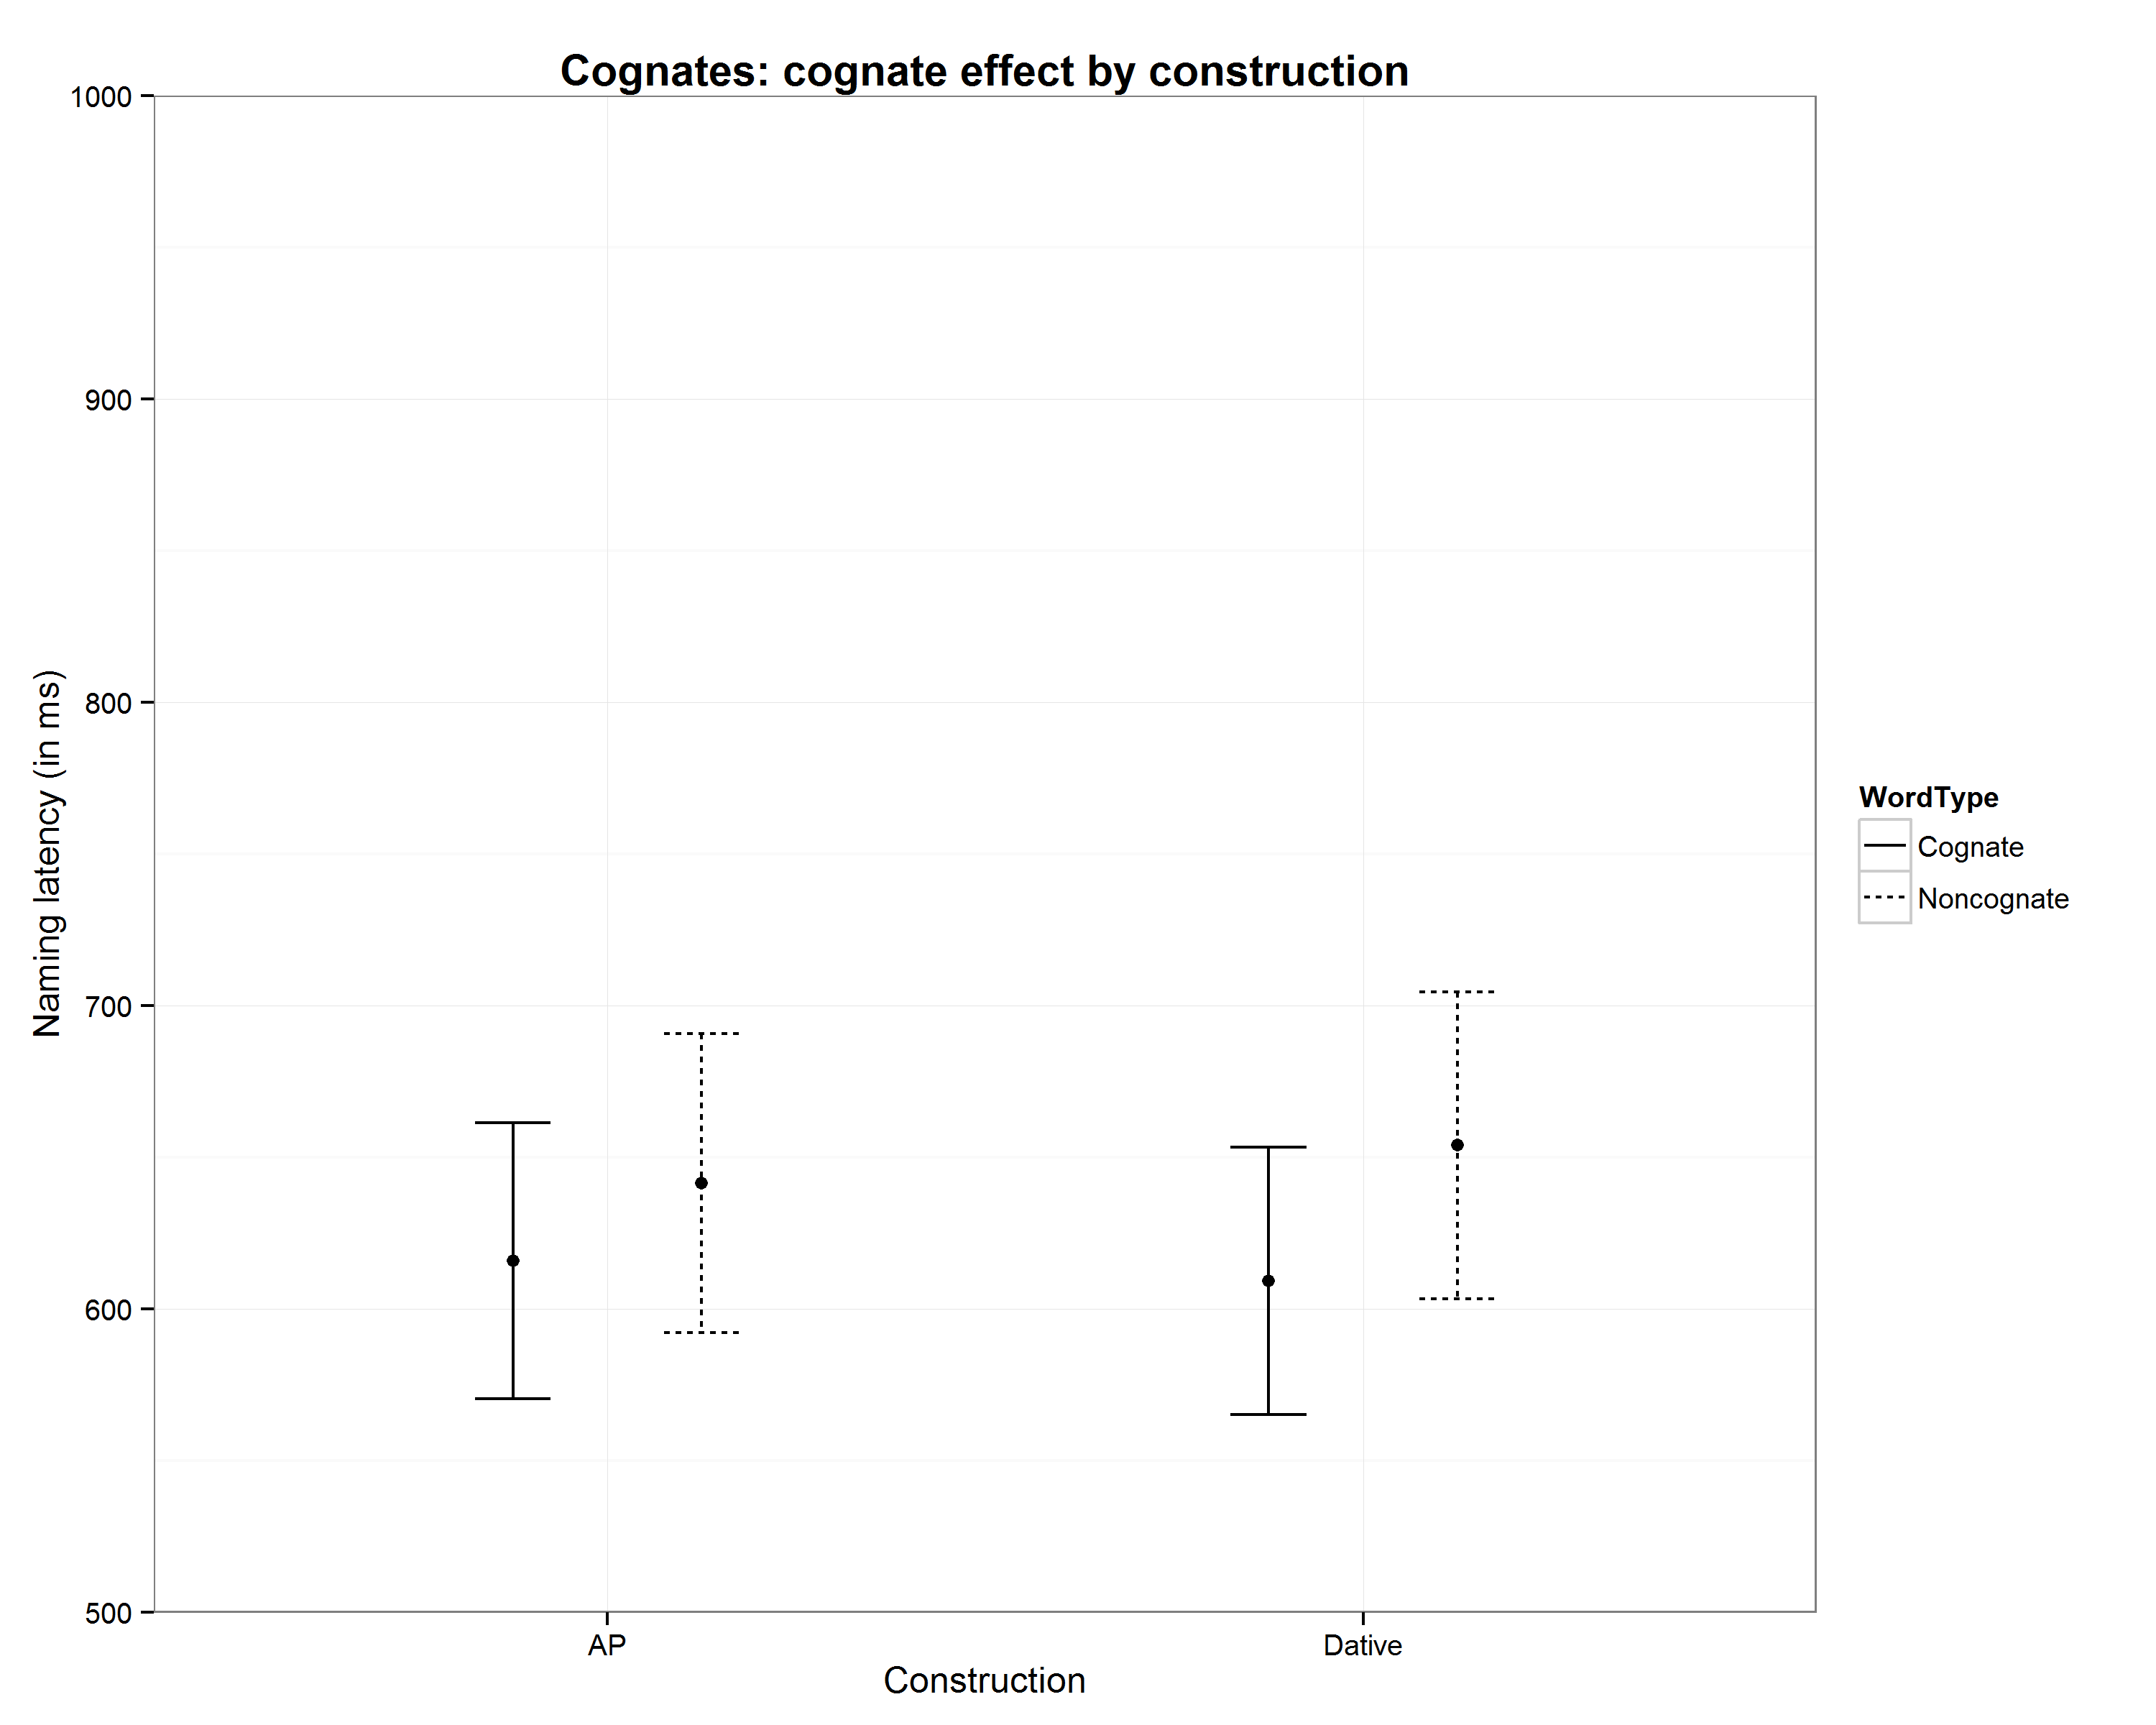
\includegraphics[width=\textwidth,height=\textheight,keepaspectratio]{conXwordtype-cogs.png}
\caption{Plotted model fits for out-of-context cognate data. Error bars depict 95\% confidence intervals.}
\label{fig:ooc.conXwordtype-cogs}
\end{figure}


For the homograph data, there was a significant effect of centered,\\ log-transformed frequency (\emph{$\beta$} = --0.024, \emph{SE} = 0.009, \emph{t} = --2.790, \emph{p} $<$ 0.01). There was no significant effect of centered word length (\emph{t} $<$ 1.96\emph{, p} $>$ 0.05). There were no significant effects for the homograph contrast, the construction contrast, nor the interaction between the two (\emph{t}s $<$ 1.96, \emph{p}s $>$ 0.05). See Table \ref{tab:ocon.bil.hom} for the fixed-effects from the homograph model, and see Figure \ref{fig:ooc.conXwordtype-homs} for a partial effects plot.

% Table generated by Excel2LaTeX from sheet 'Sheet8'
\begin{table}[htbp]
  \centering
  \caption{Fixed-effects output for the homograph out-of-context word naming model from Experiment 1.}
    \begin{tabular}{rrrrrr}
    \toprule
          & Estimate & Std..Error & t.value & p.z   & Sig. \\
    \midrule
    (Intercept) & 6.388 & 0.029 & 219.476 & 0     & * \\
    clFrequency & -0.024 & 0.009 & -2.79 & 0.005 & * \\
    cLength & 0.009 & 0.006 & 1.441 & 0.15  &  \\
    WordType & 0.019 & 0.018 & 1.022 & 0.307 &  \\
    Construction & 0.018 & 0.018 & 1     & 0.317 &  \\
    WordType:Construction & -0.026 & 0.036 & -0.728 & 0.467 &  \\
    \bottomrule
    \end{tabular}%
  \label{tab:ocon.bil.hom}%
\end{table}%

\begin{figure}[htbp]
\centering
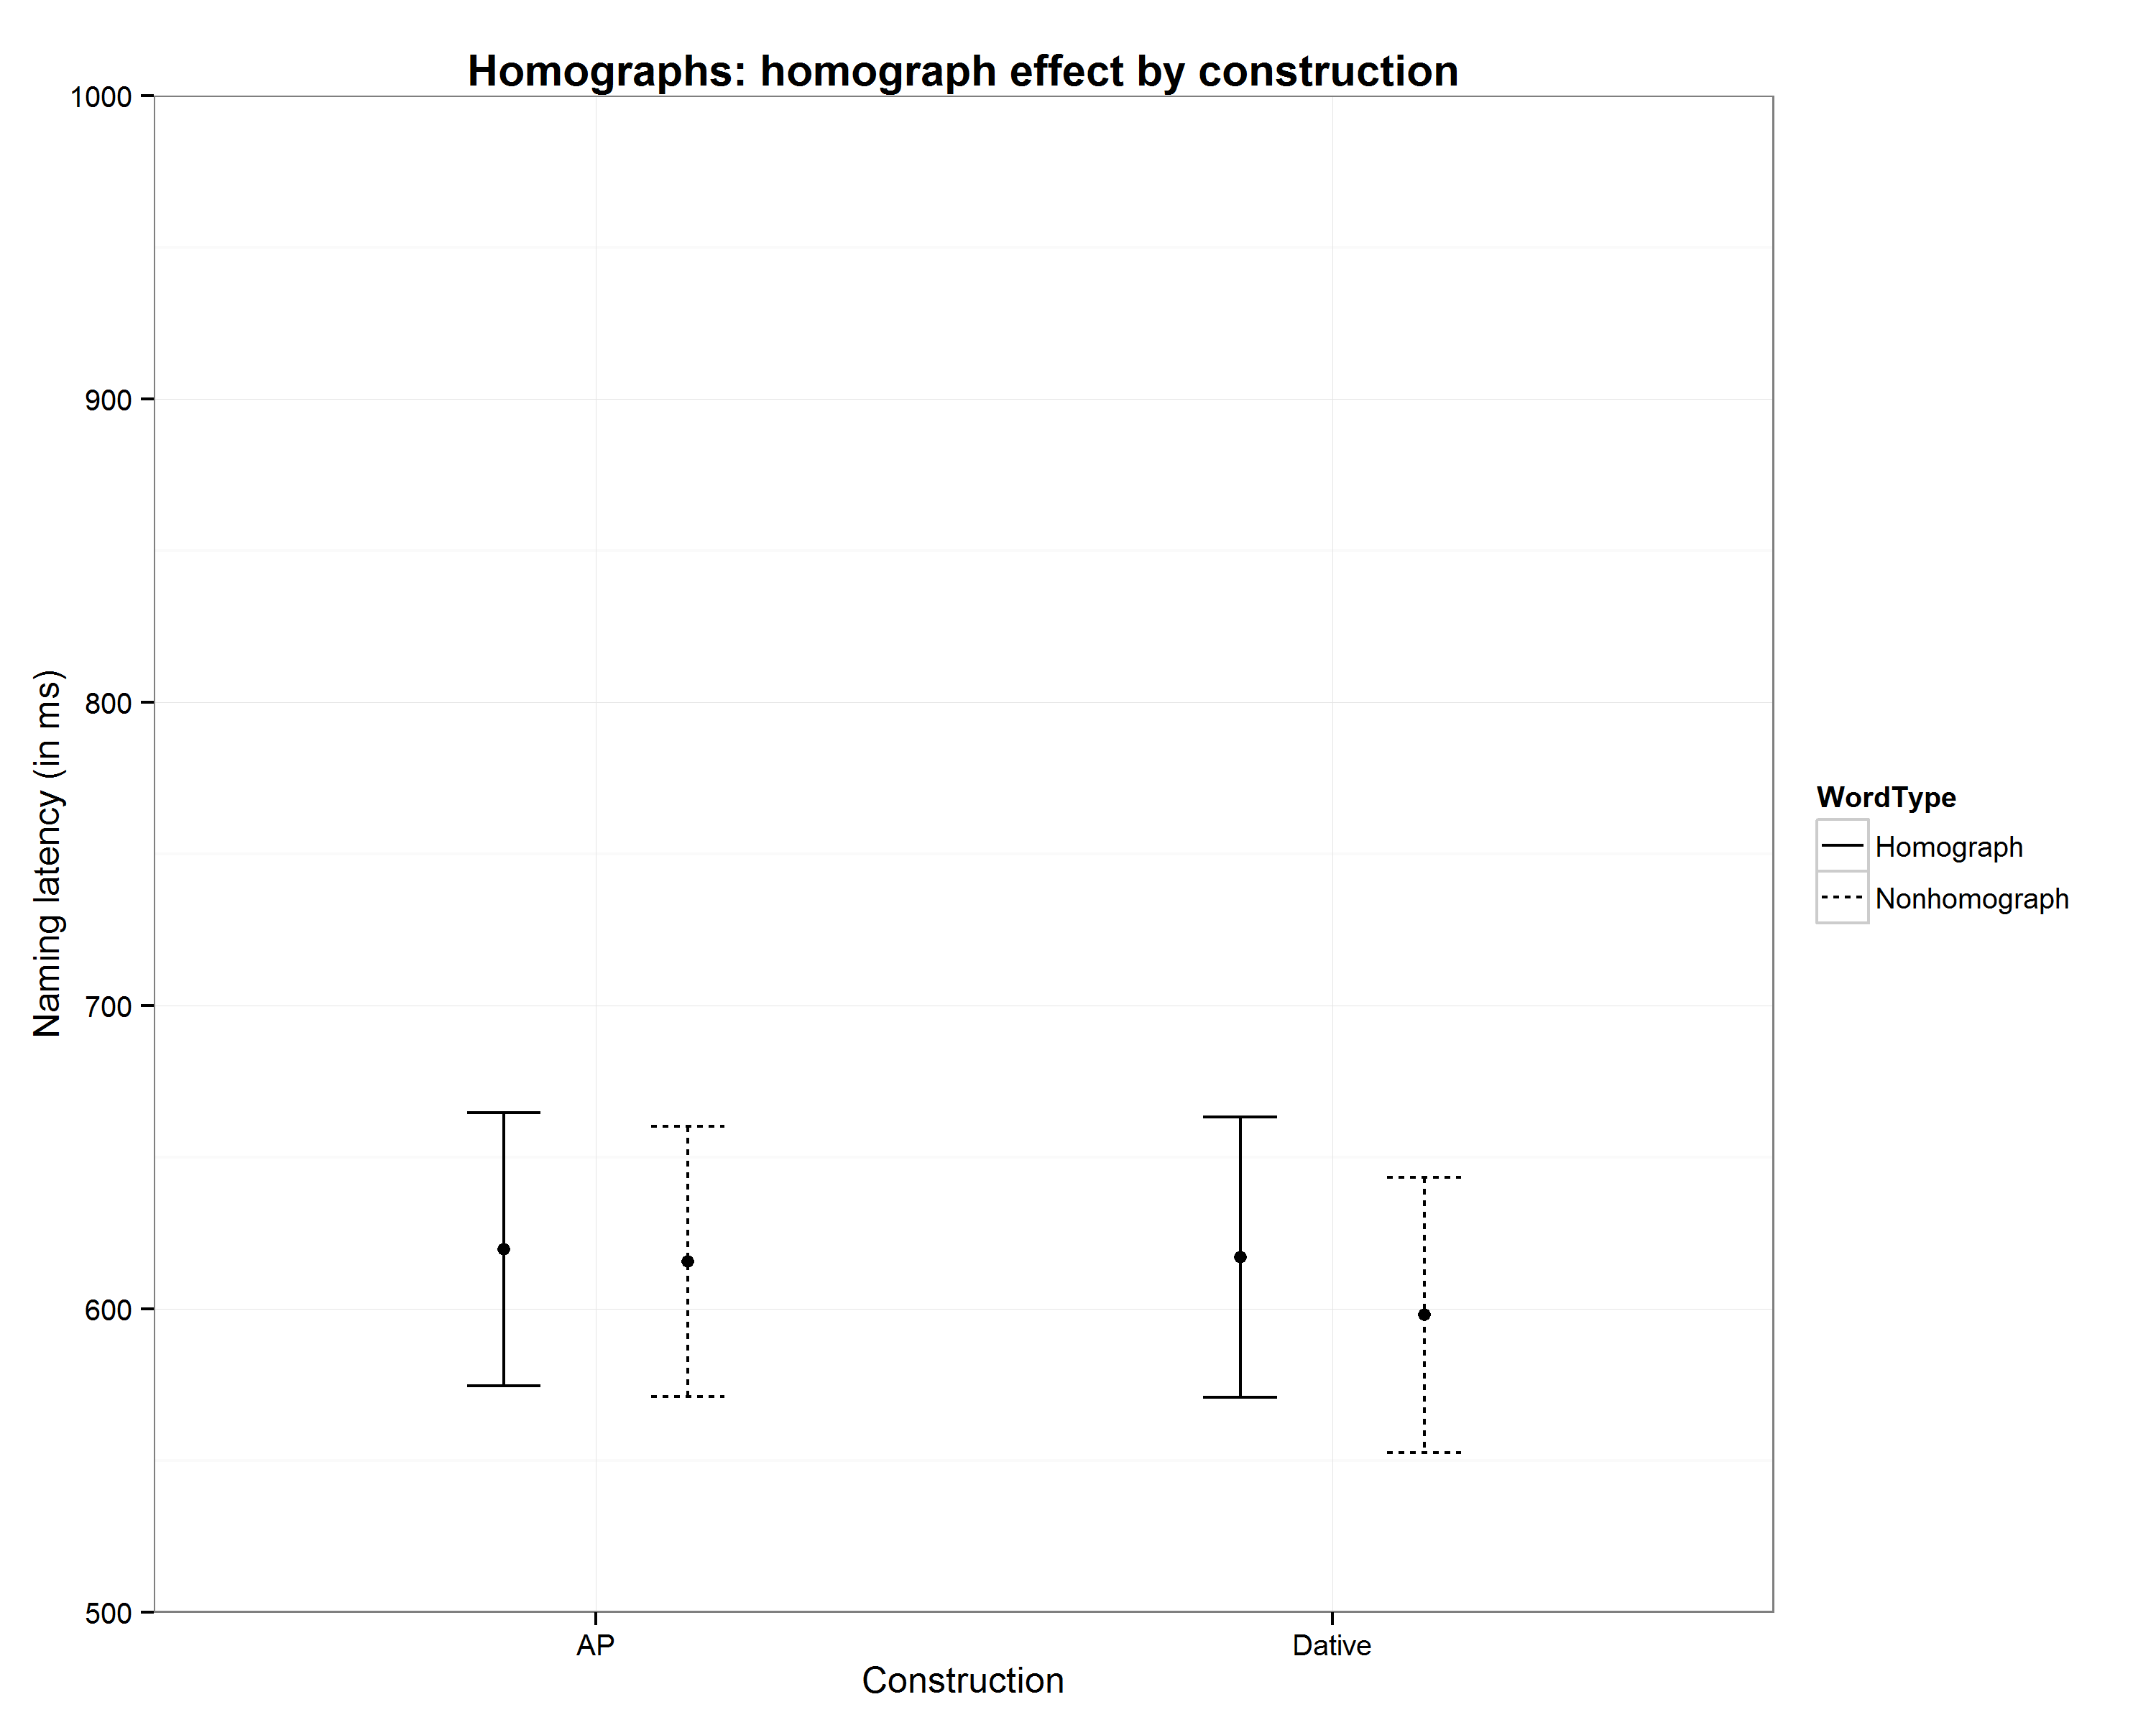
\includegraphics[width=\textwidth,height=\textheight,keepaspectratio]{conXwordtype-homs.png}
\caption{Plotted model fits for out-of-context homograph data. Error bars depict 95\% confidence intervals.}
\label{fig:ooc.conXwordtype-homs}
\end{figure}


The Spanish-English bilinguals recruited for this study showed significant cognate facilitation effect. This cognate effect was similar for the set of words that are embedded in the active and passive sentences compared to those embedded in the dative sentences in the sentence-context word naming study. These results are in line with many previous out-of-context word recognition and word naming studies finding that bilinguals co-active both languages despite performing a unilingual task. There was no evidence of a homograph inhibition effect for the bilinguals. Previous studies have shown that homograph effects are more sensitive to aspects of context, such as stimulus list composition. For example, ~\citep{Dijkstra1998} failed to observe homograph inhibition in lexical decision unless they included filler items that were in the unintended language. In this experiment, there were no items in the unintended language. A potential interpretation of the results is that bilinguals were functioning in a language selective manner, as measured by the homograph effect. 

\section{Experiment 2: Spanish-English bilinguals\\ in-context}
\label{experiment2:spanish-englishbilingualsin-context}

\subsection{Methods}
\label{methods}

\subsubsection{Participants}
\label{participants}

Forty-two Spanish-English bilinguals participated in the RSVP experiment (the final sample included 29 participants after data cleaning; see below). The participants were members of the Pennsylvania State University or the State College area communities. All participants gave informed consent, and the procedures had the approval of the Institutional Review Board of the Pennsylvania State University. Participants received \$10 per hour for their participation in the experiment. We recruited participants if they considered themselves bilingual between English and Spanish, and this recruitment procedure resulted in a heterogeneous sample of Spanish-English bilinguals with a variety of language experiences. Participants completed a language history questionnaires to assess subjective language proficiency. Additionally, a picture naming task with sections in Spanish and English, and portions of English and Spanish grammar tests (Michigan English Language Institute College English Test and the Diploma de Espa\~{n}ol como lengua extranjera) assessed objective language proficiency. Finally, an Operation-Span task ~\citep[i.e., Automatic O-Span;][]{Unsworth2005} and a Flanker Task ~\citep[e.g.,][]{Bunge2002, Emmorey2008a} assessed working memory and cognitive control. 

The recruited sample included a heterogeneous population of Spanish-English bilinguals. Some participants were born in the United States others emigrated from Spanish-speaking countries. Some participants were heritage speakers of Spanish and others knew a third language. In order to obtain a more homogeneous sample, we excluded participants from the analysis using the following procedure. We excluded participants who reported using a language other than Spanish or English (or both) at home (N=2). We also excluded participants who scored below 75\% accuracy on word naming and answering comprehension questions for the main task (N=7). We determined the cutoff of 75\% by visual inspection of histograms for word naming accuracy and comprehension question accuracy; 75\% was the point at which a second mode in the distribution began. Finally, we excluded participants from the analysis if they did not have complete data on the administered tasks (N=4) included in the final model. This resulted in a final sample of 29 participants.

% Table generated by Excel2LaTeX from sheet 'Sheet9'
\begin{table}[htbp]
  \centering
  \caption{Participant characteristics from Experiment 2.}
    \begin{tabular}{rrr}
    \toprule
    Measures & Mean  & Std. Deviation \\
    \midrule
    Age   & 24.76 & 6.86 \\
    LHQ - Average English Ratings (/10) & 8.47  & 1.39 \\
    LHQ - Average Spanish Ratings (/10) & 9.51  & 0.69 \\
    English Picture Naming (RT) & 1067.83 & 152.2 \\
    Spanish Picture Naming (RT) & 1011.86 & 192.35 \\
    English Picture Naming (ACC) & 0.84  & 0.12 \\
    Spanish Picture Naming (ACC) & 0.91  & 0.09 \\
    English Grammar Score - MELICET (out of 50) & 38.52 & 8.4 \\
    Spanish Grammar Score - DELE (out of 50) & 38.24 & 5.81 \\
    Operation Span Score (out of 60) & 42.37 & 15.07 \\
    Flanker Effect (in ms) & 48.41 & 18.39 \\
    Accuracy on Comprehension Questions & 0.88  & 0.07 \\
    \bottomrule
    \end{tabular}%
  \label{tab:incon.bil.subjchar}%
\end{table}%

Overall, the participants from the final sample were highly proficient speakers of Spanish and English and the sample showed trends toward Spanish dominance. Twenty-one participants reported using only Spanish in the home, and eight reported using both English and Spanish in the home. Participants rated themselves more highly in Spanish than in English (M$_{Spanish}$ = 9.51; M$_{English}$ = 8.47; \emph{t}(28) = 3.796, \emph{p} $<$ 0.001), and they were more accurate in the Spanish picture naming task compared to the English task (M$_{Spanish}$ = 0.91; M$_{English}$ = 0.84; \emph{t}(28) = 2.462, \emph{p} $<$ 0.05). There were no significant differences in picture naming speed (M$_{Spanish}$ = 1011.86; M$_{English}$ = 1067.83; \emph{t}(28) = 1.670, \emph{p} = 0.10) or in performance on the grammar tasks (M$_{Spanish}$ = 38.24; M$_{English}$ = 38.52; \emph{t}(22) = 0.270, \emph{p} = 0.79). The set of participant characteristics for the final sample of participants is shown in Table \ref{tab:incon.bil.subjchar}.

\subsubsection{Materials}
\label{materials}

The lexical stimuli were identical to those in Experiment 1.

We chose four structures to embed the Spanish lexical stimuli within: actives, passives, prepositional object datives structures with NP-PP word order, and prepositional object dative structures with PP-NP word order. On the basis of previous syntactic priming literature, actives, passives, and possibly NP-PP datives can be considered Spanish-non-specific structures because they have been shown to exhibit cross-language syntactic priming for Spanish and English. Prepositional object structures with PP-NP dative can be considered Spanish-specific structures because they do not share linear word order across the two languages and should exhibit less robust cross-language syntactic priming in these languages. We divided the set of cognate materials (40 cognates and 40 matched controls) and the set of homographs materials (40 cognates and 40 matched controls) in half. Half of the critical-control pairs were embedded under the active and passive sentences while the other half were embedded under the prepositional object sentences. Thus each critical and control word appeared in two sentences (active and passive, or NP-PP and PP-NP), and we created two stimulus lists to counterbalance the stimuli so that no participant saw repetitions of any critical-control word pair. This resulted in a final sample of 320 sentences with 160 sentences per list.


% Table generated by Excel2LaTeX from sheet 'Sheet10'
\begin{table}[htbp]
  \centering
  \caption{CLOZE probabilities for the sentential stimuli included in Experiment 2.}
    \begin{tabular}{rrr}
    \toprule
    Sentence Construction & Word Type & Mean CLOZE Probability \\
    \midrule
    Active & Cognate & 0.07 \\
    Active & Noncognate & 0.03 \\
    Active & Homograph & 0.03 \\
    Active & Nonhomograph & 0.03 \\
    Passive & Cognate & 0.07 \\
    Passive & Noncognate & 0.04 \\
    Passive & Homograph & 0.04 \\
    Passive & Nonhomograph & 0.06 \\
    PO(Diff) & Cognate & 0.05 \\
    PO(Diff) & Noncognate & 0.07 \\
    PO(Diff) & Homograph & 0.01 \\
    PO(Diff) & Nonhomograph & 0.02 \\
    PO(Same) & Cognate & 0.03 \\
    PO(Same) & Noncognate & 0.01 \\
    PO(Same) & Homograph & 0.02 \\
    PO(Same) & Nonhomograph & 0.01 \\
    \bottomrule
    \end{tabular}%
  \label{tab:incon.cloze}%
\end{table}%


Critical words never occurred in sentence-final position, to avoid potential sentence wrap up effects. The sentences were written with the intention to keep semantic constraint low to avoid introducing potentially confounding effects due to a highly probably target word ~\citep[e.g.,][]{Schwartz2006}. A sentence completion study confirmed that, overall the sentences had a low semantic constraint (CLOZE probability M = 0.05, range: 0.00 - 0.72), and the semantic constraint did not differ between conditions (see Table \ref{tab:incon.cloze}; all \emph{F}s $<$ 4, \emph{p}s $>$ 0.05). Care was taken to ensure that none of the words in the filler sentences overlapped with critical target words of the experimental sentences. Yes-no comprehension questions were created for each of the filler sentences and for half of the critical sentences (50\% yes, 50\% no) to probe comprehension and to further distract participants from the main goal of the task.

\subsubsection{Procedure}
\label{procedure}

The experiment lasted for two one-hour long experimental sessions that were carried out over two days. At the beginning of each session, participants gave informed consent. During the first session, they completed a language history questionnaire to gauge their language background (including subjective measures of proficiency). Participants were then seated at a computer where they began the sentence task. Sentences were presented using RSVP such that participants read sentences silently word-by-word (300 ms per word) until they encountered a target word, which was displayed in red. They were instructed to name the target word aloud quickly and accurately. Following the main task, the participants completed a test of Spanish grammar (DELE), a picture naming experiment in Spanish, and then a picture naming experiment in English. The tasks were ordered to minimize switching between the two languages, and particularly to minimize switching from English (L2) to Spanish (L1). Participants were invited back for a follow-up study during which they completed the battery of cognitive tasks (Operation Span, AXCPT, and Flanker) and a test of English grammar (MELICET).

\subsection{Results}
\label{results}

Undergraduate research assistants who spoke English and Spanish coded the accuracy of the word naming data. We excluded rials in which an incorrect word was named or in which the production would add variability to reaction times (RTs; e.g., hesitation before naming the target word) from the RT analysis. We cleaned the RT data using a procedure for the removal of absolute and relative outliers. First, considering only correctly named trials, we excluded RTs above 2500 ms and below 250 ms. We determined the absolute cutoffs via visual inspection of a density plot. Next, on the resulting subset of data, we excluded RTs if they fell outside of a 2.5 SD range around the mean naming latency for each participant. The cleaning procedure resulted in the removal of 6.5\% of correct trials. The mean comprehension question accuracy was 88\%.

Data transformations and control models were constructed following the procedure from Experiment 1. The significant control factors were centered and log-transformed word frequency, centered word length (in characters), and a composite score of picture naming performance (summed z-scores of inverse reaction time and accuracy on the picture naming task). These effects made up the control model. On top of the control model, we added the a-priori effects of interest. The primary effects of interest were two categorical variables: sentence construction (active, passive, NP-PP dative, and PP-NP dative) and word type (cognate, non-cognate control, homograph, non-homograph control), and their interaction. Because the sets of cognates and controls and homographs and controls are not comparable (they were not matched to each other), we constructed two separate models to examine the cognate effect (cognate vs. non-cognate) and the homograph effect (homograph vs. non-homograph) independently. We used sum coding for for each word-type contrast. The categorical variable for sentence construction was contrast coded to yield three orthogonal comparisons: active sentences, NP-PP dative sentences, and PP-NP dative sentences compared to passive sentences; NP-PP datives and PP-NP datives compared to active sentences; and PP-NP dative compared to NP-PP datives. 

After we constructed the effects-of-interest models, we tested for interactions between individual difference variables of executive control and language fluency and the effects of interest. Previous studies have shown that variables tracking language fluency interact with the magnitude of the cognate effect and variables tracking executive function interact with the homograph effect. Significance was tested via removal of the interaction terms during model comparison. 

For the random effects structure of the final models (the a priori models and the individual differences models), ``keep it maximal'' ~\citep{Barr2013} by including random intercepts for participants and items and by adding random slopes for all between-participant variables by item and all between-item variables by participant. If a model failed to converge random slopes were removed; at a minimum random slopes for word type, construction, and the interaction between construction and word type were added by participant, and a random slope (and correlations with the intercept) for the Spanish naming composite was added by target word. 

\subsubsection{Cognate analysis}
\label{cognateanalysis}

The results of the cognate model are as follows. There was an effect of Spanish picture naming composite, such that an increase in the composite (related to increased fluency in Spanish) related to a decrease in log RT (\emph{$\beta$} = --0.084, \emph{SE} = 0.023, \emph{t} = --3.682, \emph{p} $<$ 0.001). There was an effect of centered log word frequency, such that an increase in frequency related to a decrease in log RT (\emph{$\beta$} = --0.013, \emph{SE} = 0.004, \emph{t} = --2.984, \emph{p} $<$ 0.01). There was an effect of centered word length, such that an increase in number of characters related to an increase in log RT ($\beta$ = 0.013, \emph{SE} = 0.003, \emph{t} = 4.739, p $<$ 0.001). There was an effect for the contrast between passive and all other structures, such that words named in passive sentences were named more quickly compared to active sentences (\emph{$\beta$} = --0.011, \emph{SE} = 0.003, \emph{t} = --4.317, \emph{p} $<$ 0.001). There was no effect of the contrast between the two dative structures and active structure nor for the contrast between the two dative structures (\emph{t} $<$ 1, \emph{p}, $>$ 0.05). There was an effect for the cognate contrast such that, cognates were named more quickly compared to non-cognate controls (\emph{$\beta$} = 0.055, \emph{SE} = 0.016, \emph{t} = 3.482, \emph{p} $<$ 0.001). The cognate contrast interacted with Spanish picture naming composite, such that the magnitude of the cognate effect decreased with an increase in the composite (related to increasing Spanish fluency; \emph{$\beta$} = --0.034, \emph{SE} = 0.010, \emph{t} = --3.419, \emph{p} $<$ 0.001). The cognate contrast also interacted with the contrast between the two dative structures, indicating that the cognate effect was larger in dative sentences with NP-PP word order compared to sentences with PP-NP word order (\emph{$\beta$} = --0.024, \emph{SE} = 0.012, \emph{t} = --2.044, \emph{p} $<$ 0.05). The cognate contrast did not interact with any other sentence construction contrast (\emph{t}s $<$ 1, \emph{p}s $>$ 0.05) There was no evidence for the addition of a three way interaction between Spanish composite, cognate contrast, and sentence structure in the model ($\chi^2$ (6) = 7.245, p = 0.29). See Table \ref{tab:incon.bil.cognatemodel} for the fixed-effects from the cognate model, and see Figure \ref{fig:Rplot34} for a partial effects plot. 

\begin{figure}[htbp]
\centering
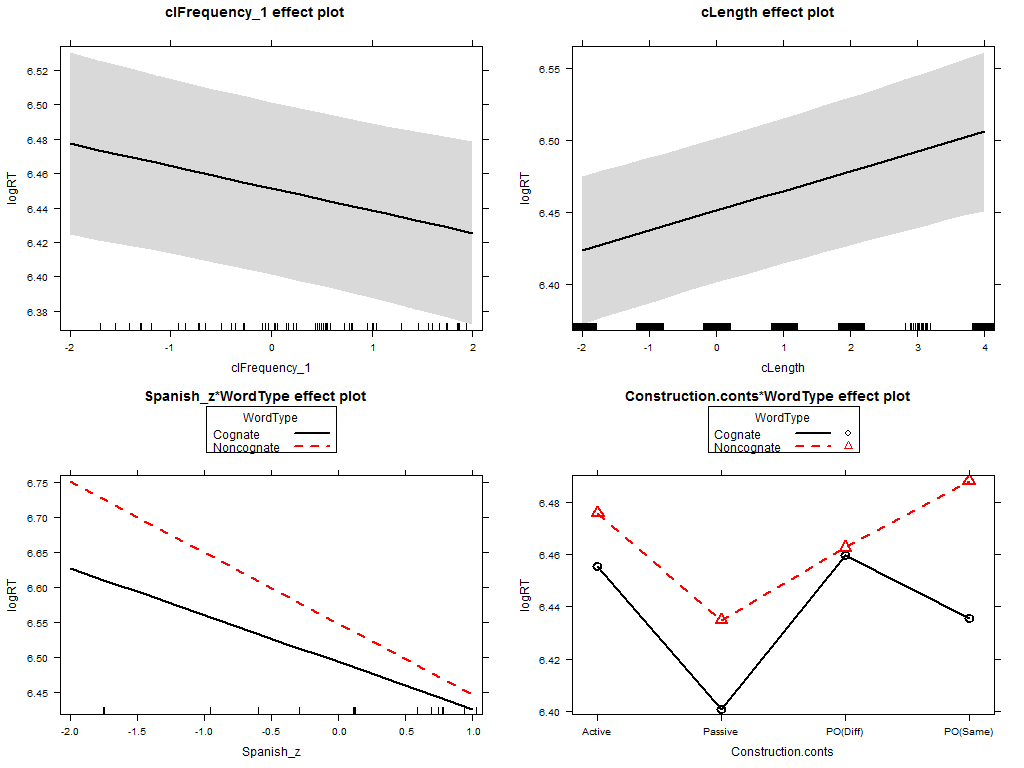
\includegraphics[width=\textwidth,height=\textheight,keepaspectratio]{Rplot34.png}
\caption{Plotted model fits for in-context cognate data. The y-axis is log reaction time. clFrequency\_1 is mean-centered log word frequency; cLength is mean-centered word length, Spanish\_z is the z-score Spanish fluency picture naming composite, and Construction.conts represents the different construction conditions.}
\label{fig:Rplot34}
\end{figure}


To explore possible interactions between cognitive control, language fluency, and language co-activation, we tested for higher-order interactions between cognitive control variables (AXCPT ratio of proactive control, OSpan z-score, and the Flanker effect z-score) and the cognate and construction contrasts, and between the Spanish picture naming composite and cognate and the construction contrasts. We evaluated significance for the interactions by model comparison to less complex models. This procedure resulted in the removal of 5 participants who did not have complete data on the tasks. There was no evidence for higher order interactions between executive control variables, the cognate contrast, and sentence construction (\emph{p} $>$ 0.05 on all $\chi^2$ tests of model comparison).

% Table generated by Excel2LaTeX from sheet 'Sheet11'
\begin{landscape}
\begin{table}[htbp]
  \centering
  \caption{Fixed-effects output for the cognate in-context model in Experiment 2.}
    \begin{tabular}{rrrrrr}
    \toprule
          & Estimate & Std..Error & t.value & p.z   & Sig. \\
    \midrule
    (Intercept) & 6.52  & 0.032 & 206.239 & 0     & * \\
    Construction.contsAll\_Act.V.Passive & -0.011 & 0.003 & -4.318 & 0     & * \\
    Construction.contsDats.V.Active & 0.001 & 0.004 & 0.322 & 0.747 &  \\
    Construction.contsNP-PP.V.PP-NP & 0     & 0.007 & -0.054 & 0.957 &  \\
    Spanish\_z & -0.084 & 0.023 & -3.682 & 0     & * \\
    WordTypeCog.V.Ncog & 0.055 & 0.016 & 3.482 & 0     & * \\
    clFrequency\_1 & -0.013 & 0.004 & -2.985 & 0.003 & * \\
    cLength & 0.014 & 0.003 & 4.74  & 0     & * \\
    Spanish\_z:WordTypeCog.V.Ncog & -0.034 & 0.01  & -3.42 & 0.001 & * \\
    Construction.contsAll\_Act.V.Passive:WordTypeCog.V.Ncog & 0.002 & 0.005 & 0.402 & 0.688 &  \\
    Construction.contsDats.V.Active:WordTypeCog.V.Ncog & -0.002 & 0.009 & -0.268 & 0.789 &  \\
    Construction.contsNP-PP.V.PP-NP:WordTypeCog.V.Ncog & -0.025 & 0.012 & -2.045 & 0.041 & * \\
    \bottomrule
    \end{tabular}%
  \label{tab:incon.bil.cognatemodel}%
\end{table}%
\end{landscape}


\subsubsection{Homograph analysis}
\label{homographanalysis}

The results of the homograph model are as follows. There was an effect of Spanish picture naming composite, such that an increase in the composite (related to increased fluency in Spanish) related to a decrease in log RT (\emph{$\beta$} = --0.058, \emph{SE} = 0.023, \emph{t} = --2.450, \emph{p} $<$ 0.05). There was an effect of centered log word frequency, such that an increase in frequency related to a decrease in log RT (\emph{$\beta$} = --0.026, \emph{SE} = 0.005, \emph{t} = --4.567, \emph{p} $<$ 0.001). There no significant effect of centered word length (\emph{t} $<$ 1, \emph{p $>$} 0.05). There was an effect for the contrast between passive and all other structures, such that words named in passive sentences were named more quickly compared to active sentences (\emph{$\beta$} = --0.012, \emph{SE} = 0.004, \emph{t} = --3.099, \emph{p} $<$ 0.01). There was no effect of the contrast between the two dative structures and active structure nor for the contrast between the two dative structures (\emph{t} $<$ 1, \emph{p} $>$ 0.05). There was no effect for the homograph contrast, and no interaction between Spanish naming composite and the homograph contrast (\emph{t}s $<$ 1, \emph{p}s $>$ 0.05). However, the homograph contrast contrast interacted with the contrast between the active structure and the two dative structures, indicating that there was significant homograph inhibition in the dative structures (\emph{$\beta$} = --0.025, \emph{SE} = 0.010, \emph{t} = 2.40., \emph{p} $<$ 0.05). The homograph contrast did not interact with any other sentence construction contrast (\emph{t}s $<$ 1, \emph{p}s $>$ 0.05). There was no evidence for the addition of a three way interaction between Spanish composite, homograph contrast, and sentence structure in the model ($\chi^2$ (6) = 9.312, p = 0.156). See Table \ref{tab:incon.bil.homographmodel} for the fixed-effects from the homograph model, and see Figure \ref{fig:Rplot35} for a partial effects plot.

\begin{figure}[htbp]
\centering
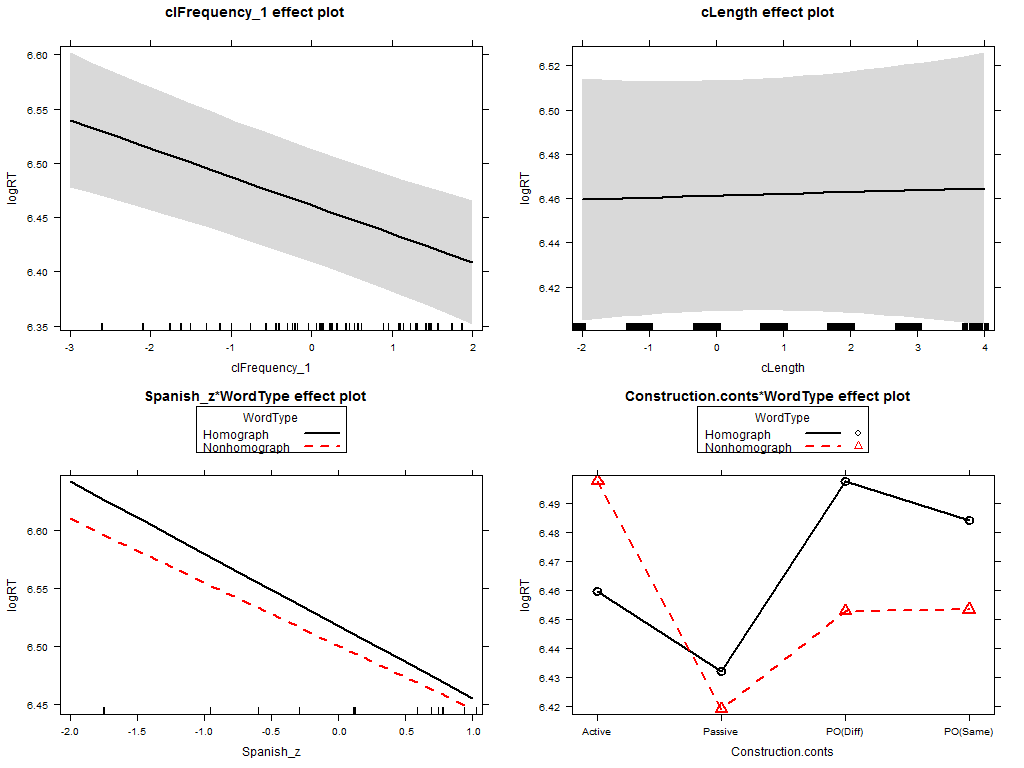
\includegraphics[width=\textwidth,height=\textheight,keepaspectratio]{Rplot35.png}
\caption{Plotted model fits for in-context homograph data. The y-axis is log reaction time. clFrequency\_1 is mean-centered log word frequency; cLength is mean-centered word length, Spanish\_z is the z-score Spanish fluency picture naming composite, and Construction.conts represents the different construction conditions.}
\label{fig:Rplot35}
\end{figure}

To explore possible interactions between cognitive control, language fluency, and language co-activation, we tested for higher-order interactions between cognitive control variables (AXCPT ratio of proactive control, OSpan z-score, and the Flanker effect z-score) and the homograph and construction contrasts, and between the Spanish picture naming composite and homograph and the construction contrasts. We evaluated significance for the interactions by model comparison to less complex models. This procedure resulted in the removal of 5 participants who did not have complete data on the tasks. There was no evidence for higher order interactions between executive control variables, the homograph contrast, and sentence construction (p $>$ 0.05 on all $\chi^2$ tests of model comparison).



\begin{landscape}
% Table generated by Excel2LaTeX from sheet 'Sheet12'
\begin{table}[htbp]
  \centering
  \caption{Fixed-effects output for the homograph in-context model in Experiment 2.}
    \begin{tabular}{rrrrrr}
    \toprule
          & Estimate & Std..Error & t.value & p.z   & Sig. \\
    \midrule
    (Intercept) & 6.51  & 0.033 & 197.294 & 0     & * \\
    Construction.contsAll\_Act.V.Passive & -0.012 & 0.004 & -3.1  & 0.002 & * \\
    Construction.contsDats.V.Active & 0.002 & 0.005 & 0.449 & 0.654 &  \\
    Construction.contsNP-PP.V.PP-NP & 0.003 & 0.008 & 0.378 & 0.705 &  \\
    Spanish\_z & -0.059 & 0.024 & -2.45 & 0.014 & * \\
    WordTypeHom.V.Ncog & -0.019 & 0.018 & -1.034 & 0.301 &  \\
    clFrequency\_1 & -0.026 & 0.006 & -4.568 & 0     & * \\
    cLength & 0.001 & 0.004 & 0.206 & 0.837 &  \\
    Spanish\_z:WordTypeHom.V.Ncog & 0.008 & 0.011 & 0.721 & 0.471 &  \\
    Construction.contsAll\_Act.V.Passive:WordTypeHom.V.Ncog & 0     & 0.006 & -0.026 & 0.979 &  \\
    Construction.contsDats.V.Active:WordTypeHom.V.Ncog & 0.025 & 0.01  & 2.403 & 0.016 & * \\
    Construction.contsNP-PP.V.PP-NP:WordTypeHom.V.Ncog & -0.007 & 0.016 & -0.435 & 0.664 &  \\
    \bottomrule
    \end{tabular}%
  \label{tab:incon.bil.homographmodel}%
\end{table}%
\end{landscape}



\subsubsection{Reanalysis of Experiments 1 and 2}
\label{reanalysisofexperiments1and2}

Experiment 1 showed significant cognate facilitation but no homograph inhibition outside of sentence context. In Experiment 2, the cognate facilitation and homograph inhibition effects were present and modulated by sentence construction. A potential explanation of this modulation is that there were lexical confounds across the construction conditions that were not detected by the out-of-context analysis. This could be the case particularly for the homograph stimuli given a curious lack of homograph inhibition effect out-of-context. While it is temping to explain the lack of homograph inhibition in Experiment 1 as due to the monolingual, Spanish nature of the task (i.e., there were no English distractor words to induce activation of English), the were cognate words that did activate the unintended language, the participants were balanced in the use of their two languages but living or working in an English dominant environment, and the participants spoke English with the experimenter before proceeding with the word naming portion of the study. Thus, the homographs should have produced inhibitory effects but may have contained stimuli with unintended lexical confounds, increasing variability and masking an effect.

To ensure that the apparent interactions between word type (particularly homograph effects) and construction were not due to lexical effects across the two sets of items (e.g., ``inefficient'' cognate or homograph items present to a greater degree in the dative condition), we conduced a conditional reanalysis of the data in the first two experiments. We subsetted the data from Experiments 1 and 2 to include on those critical-control word pairs which showed the predicted cognate facilitation or homograph inhibition effect in the out of context task in Experiment 1. To this end, we calculated mean naming latencies for each critical - control word pair. We visually inspected critical-control pairs; we treated any cognate-control pairs with a mean difference less than 0 as showing cognate facilitation, and any homograph-control pair with a mean difference greater than 0 as showing homograph inhibition. We excluded and any item pairs that did not fit into either of these conditions from the reanalysis. Thus, the reanalysis of Experiments 1 and 2 included only items that were shown to elicit cognate and homograph effects outside of sentence context. This process resulted in the removal of 11 cognate-control word pairs (5 from active and passive, and 6 from dative conditions) and 11 homograph-control word pairs (7 from active and passive, and 6 from dative conditions), about 25\% of the observations from the cognate model and 27\% from the homograph model. 

\paragraph{Reanalysis of Experiment 1:\\ Spanish-English bilinguals out-of-context\\}
\label{reanalysisofexperiment1:spanish-englishbilingualsout-of-context}

The models from Experiment 1 were recomputed after calculating and removing item-specific cognate and homograph effects. For the cognate data, there was a significant effect of centered log-transformed word frequency (\emph{$\beta$} = --0.022, \emph{SE} = 0.006, \emph{t} = --3.746, \emph{p} $<$ 0.001), indicating that an increase in word frequency related to a decrease in log RT. There was also an effect of centered word length (\emph{$\beta$} = 0.022, \emph{SE} = 0.004, \emph{t} = 6.210, \emph{p} $<$ 0.001), indicating that an increase in word length related to an increase in log RT. There was significant effect of the cognate contrast (\emph{$\beta$} = --0.084, \emph{SE} = 0.015, \emph{t} = --5.491, \emph{p} $<$ 0.001), indicating that cognates were named more quickly compared to non-cognate controls. There was no significant effect of the construction contrast, (\emph{t} $<$ 1, \emph{p}s $>$ 0.05). The interaction between the cognate contrast and the construction contrast approached significance (\emph{$\beta$} = 0.048, \emph{SE} = 0.028, \emph{t} = 1.710, \emph{p} = 0.08), indicating that if anything, the cognate effect in the dative condition was larger than the cognate effect in the active and passive condition. See Table \ref{tab:ocon.cog.reanl} for the fixed-effects from the cognate model, and see Figure \ref{fig:conXwordtype-cogs-excluded} for a partial effects plot. 

\begin{figure}[htbp]
\centering
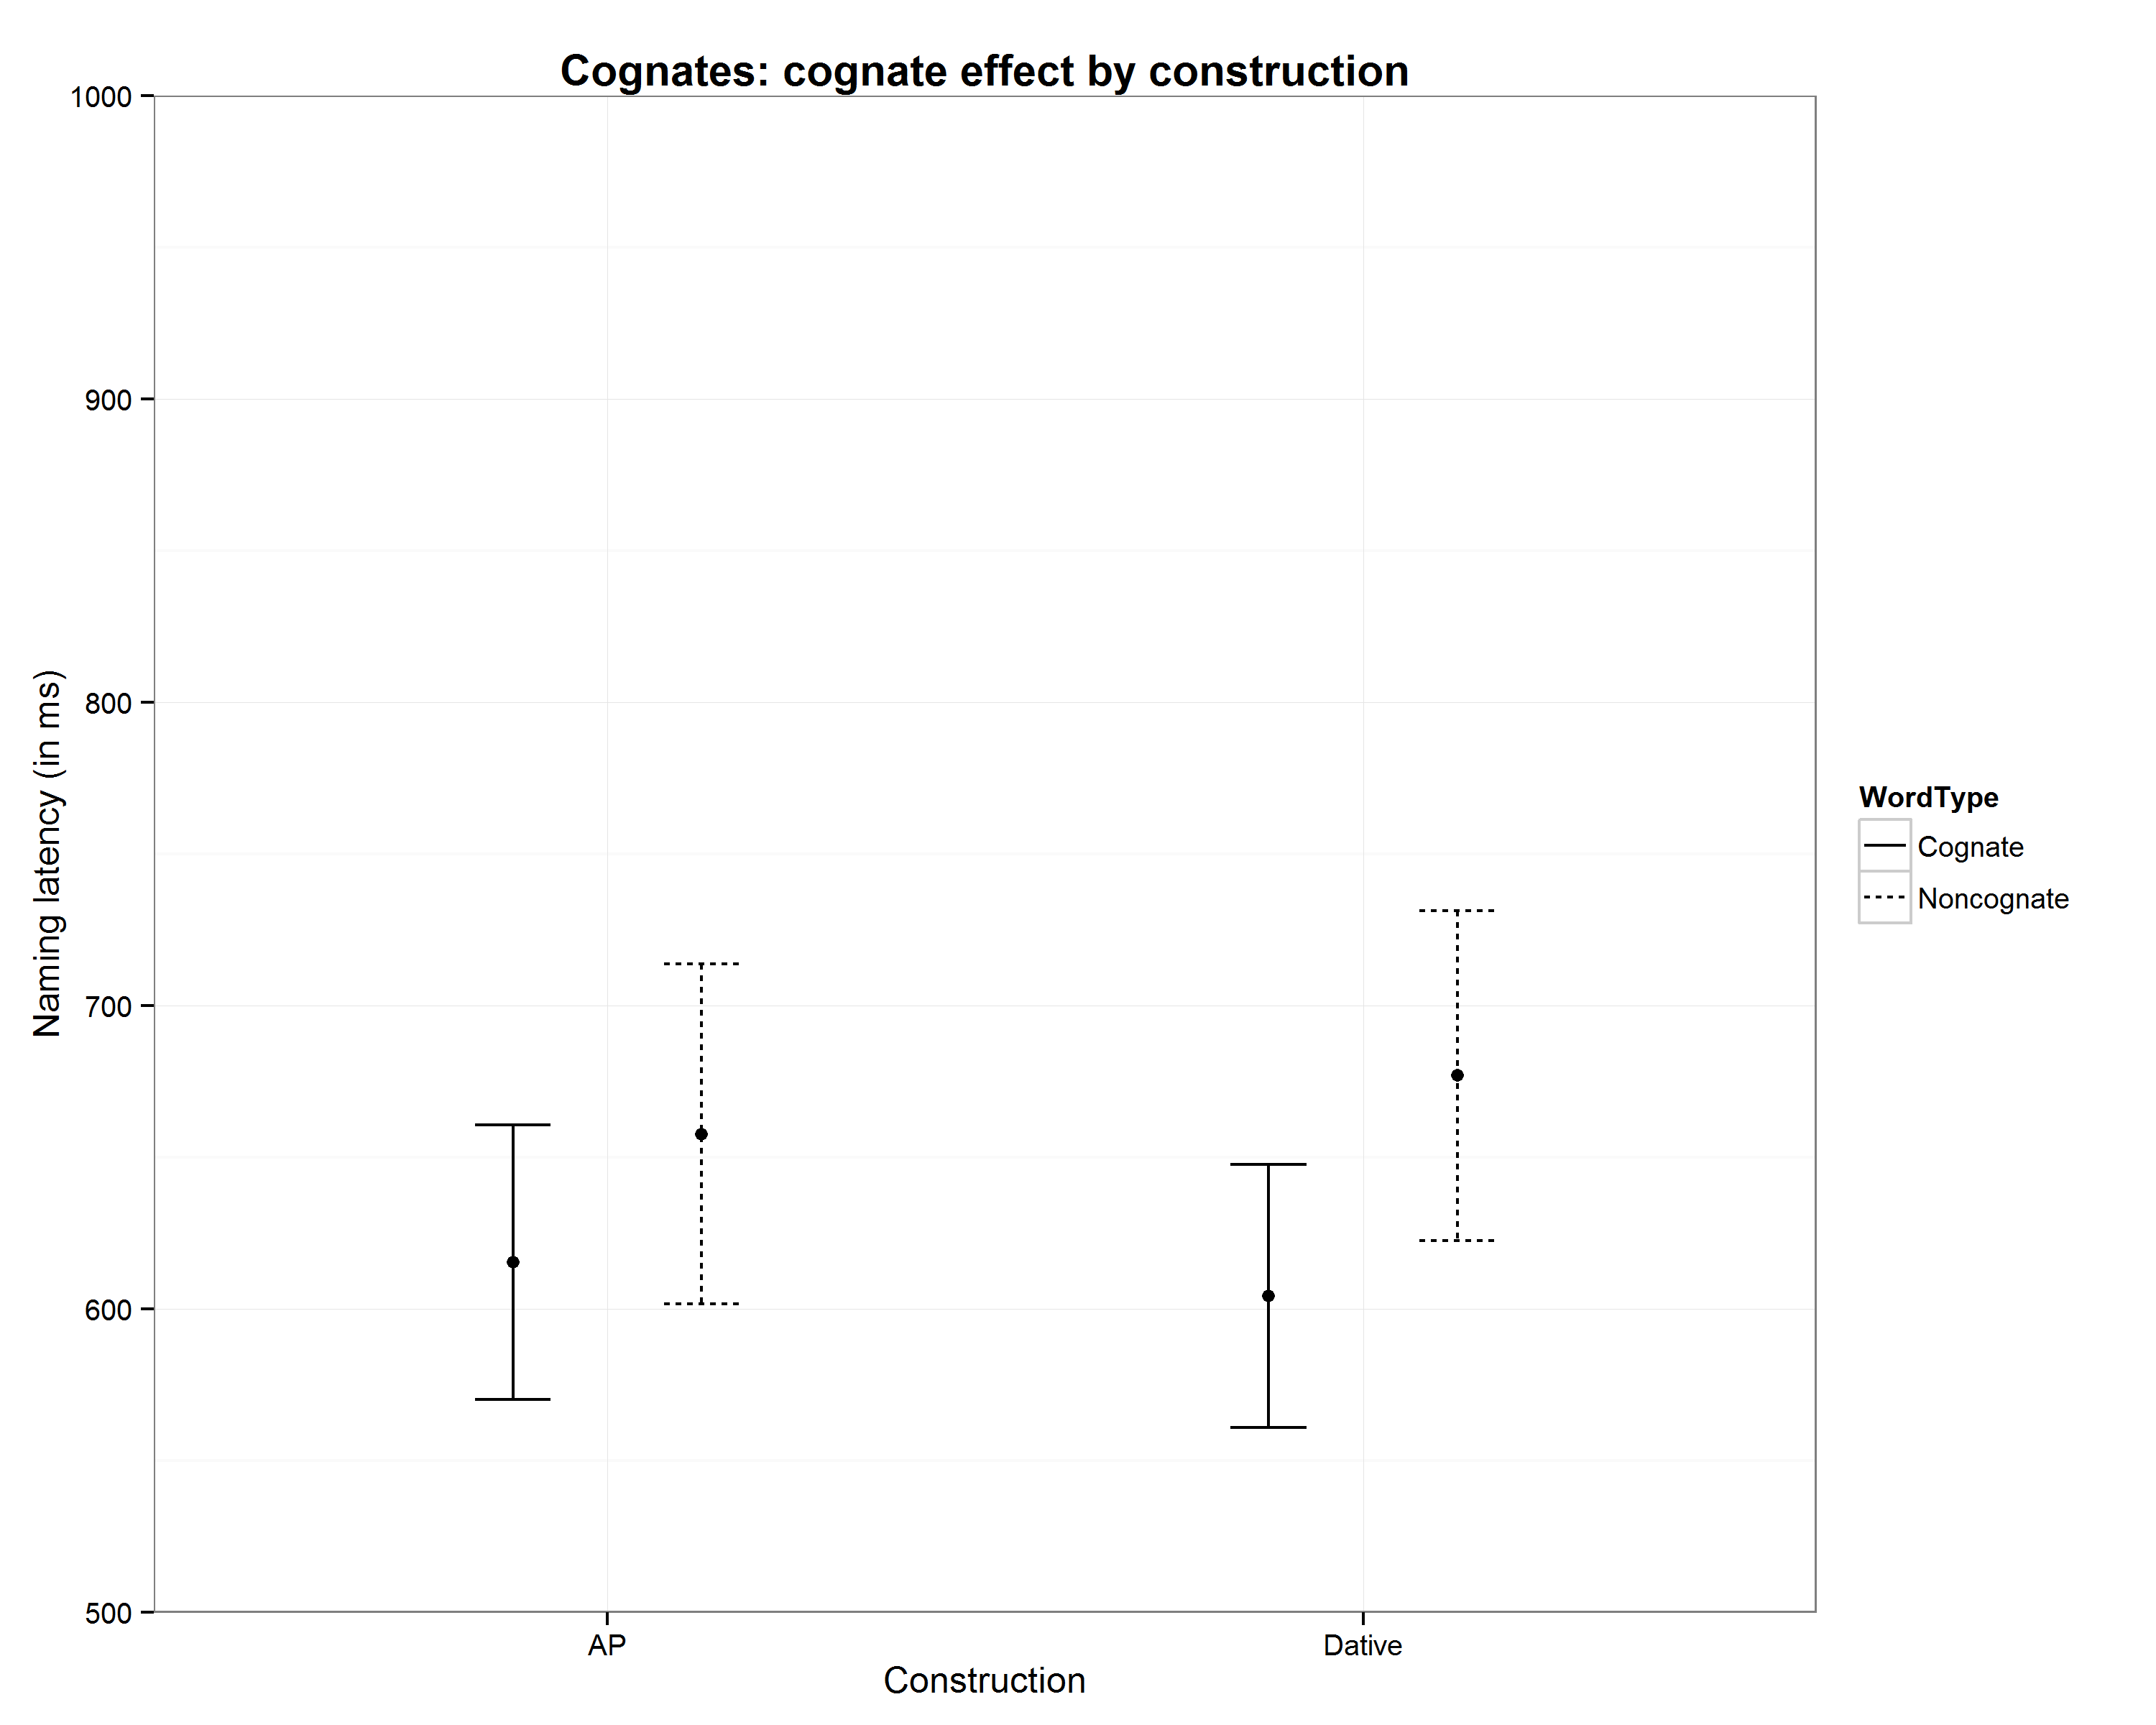
\includegraphics[width=\textwidth,height=\textheight,keepaspectratio]{conXwordtype-cogs-excluded.png}
\caption{Plotted model fits for out-of-context cognate data after reanalysis in which item pairs that did not show cognate facilitation were excluded. Error bars depict 95\% confidence intervals.}
\label{fig:conXwordtype-cogs-excluded}
\end{figure}

For the homograph data, there was a significant effect of centered,\\ log-transformed frequency (\emph{$\beta$} = --0.047, \emph{SE} = 0.009, \emph{t} = --5.161, \emph{p} $<$ 0.001). There was no significant effect of centered word length (\emph{t} $<$ 1, \emph{p} $>$ 0.05). There was a significant effect of the homograph contrast (\emph{$\beta$} = 0.072, \emph{SE} = 0.020, \emph{t} = 3.714, \emph{p} $<$ 0.001), indicating that homograph were named more slowly than controls. Neither the construction contrast nor the interaction between construction and word type were significant (\emph{t}s $<$ 1.96, \emph{p}s $>$ 0.05). See Table \ref{tab:ocon.hom.reanl} for the fixed-effects from the homograph model, and see Figure \ref{fig:conXwordtype-homs-excluded} for a partial effects plot. 

\begin{figure}[htbp]
\centering
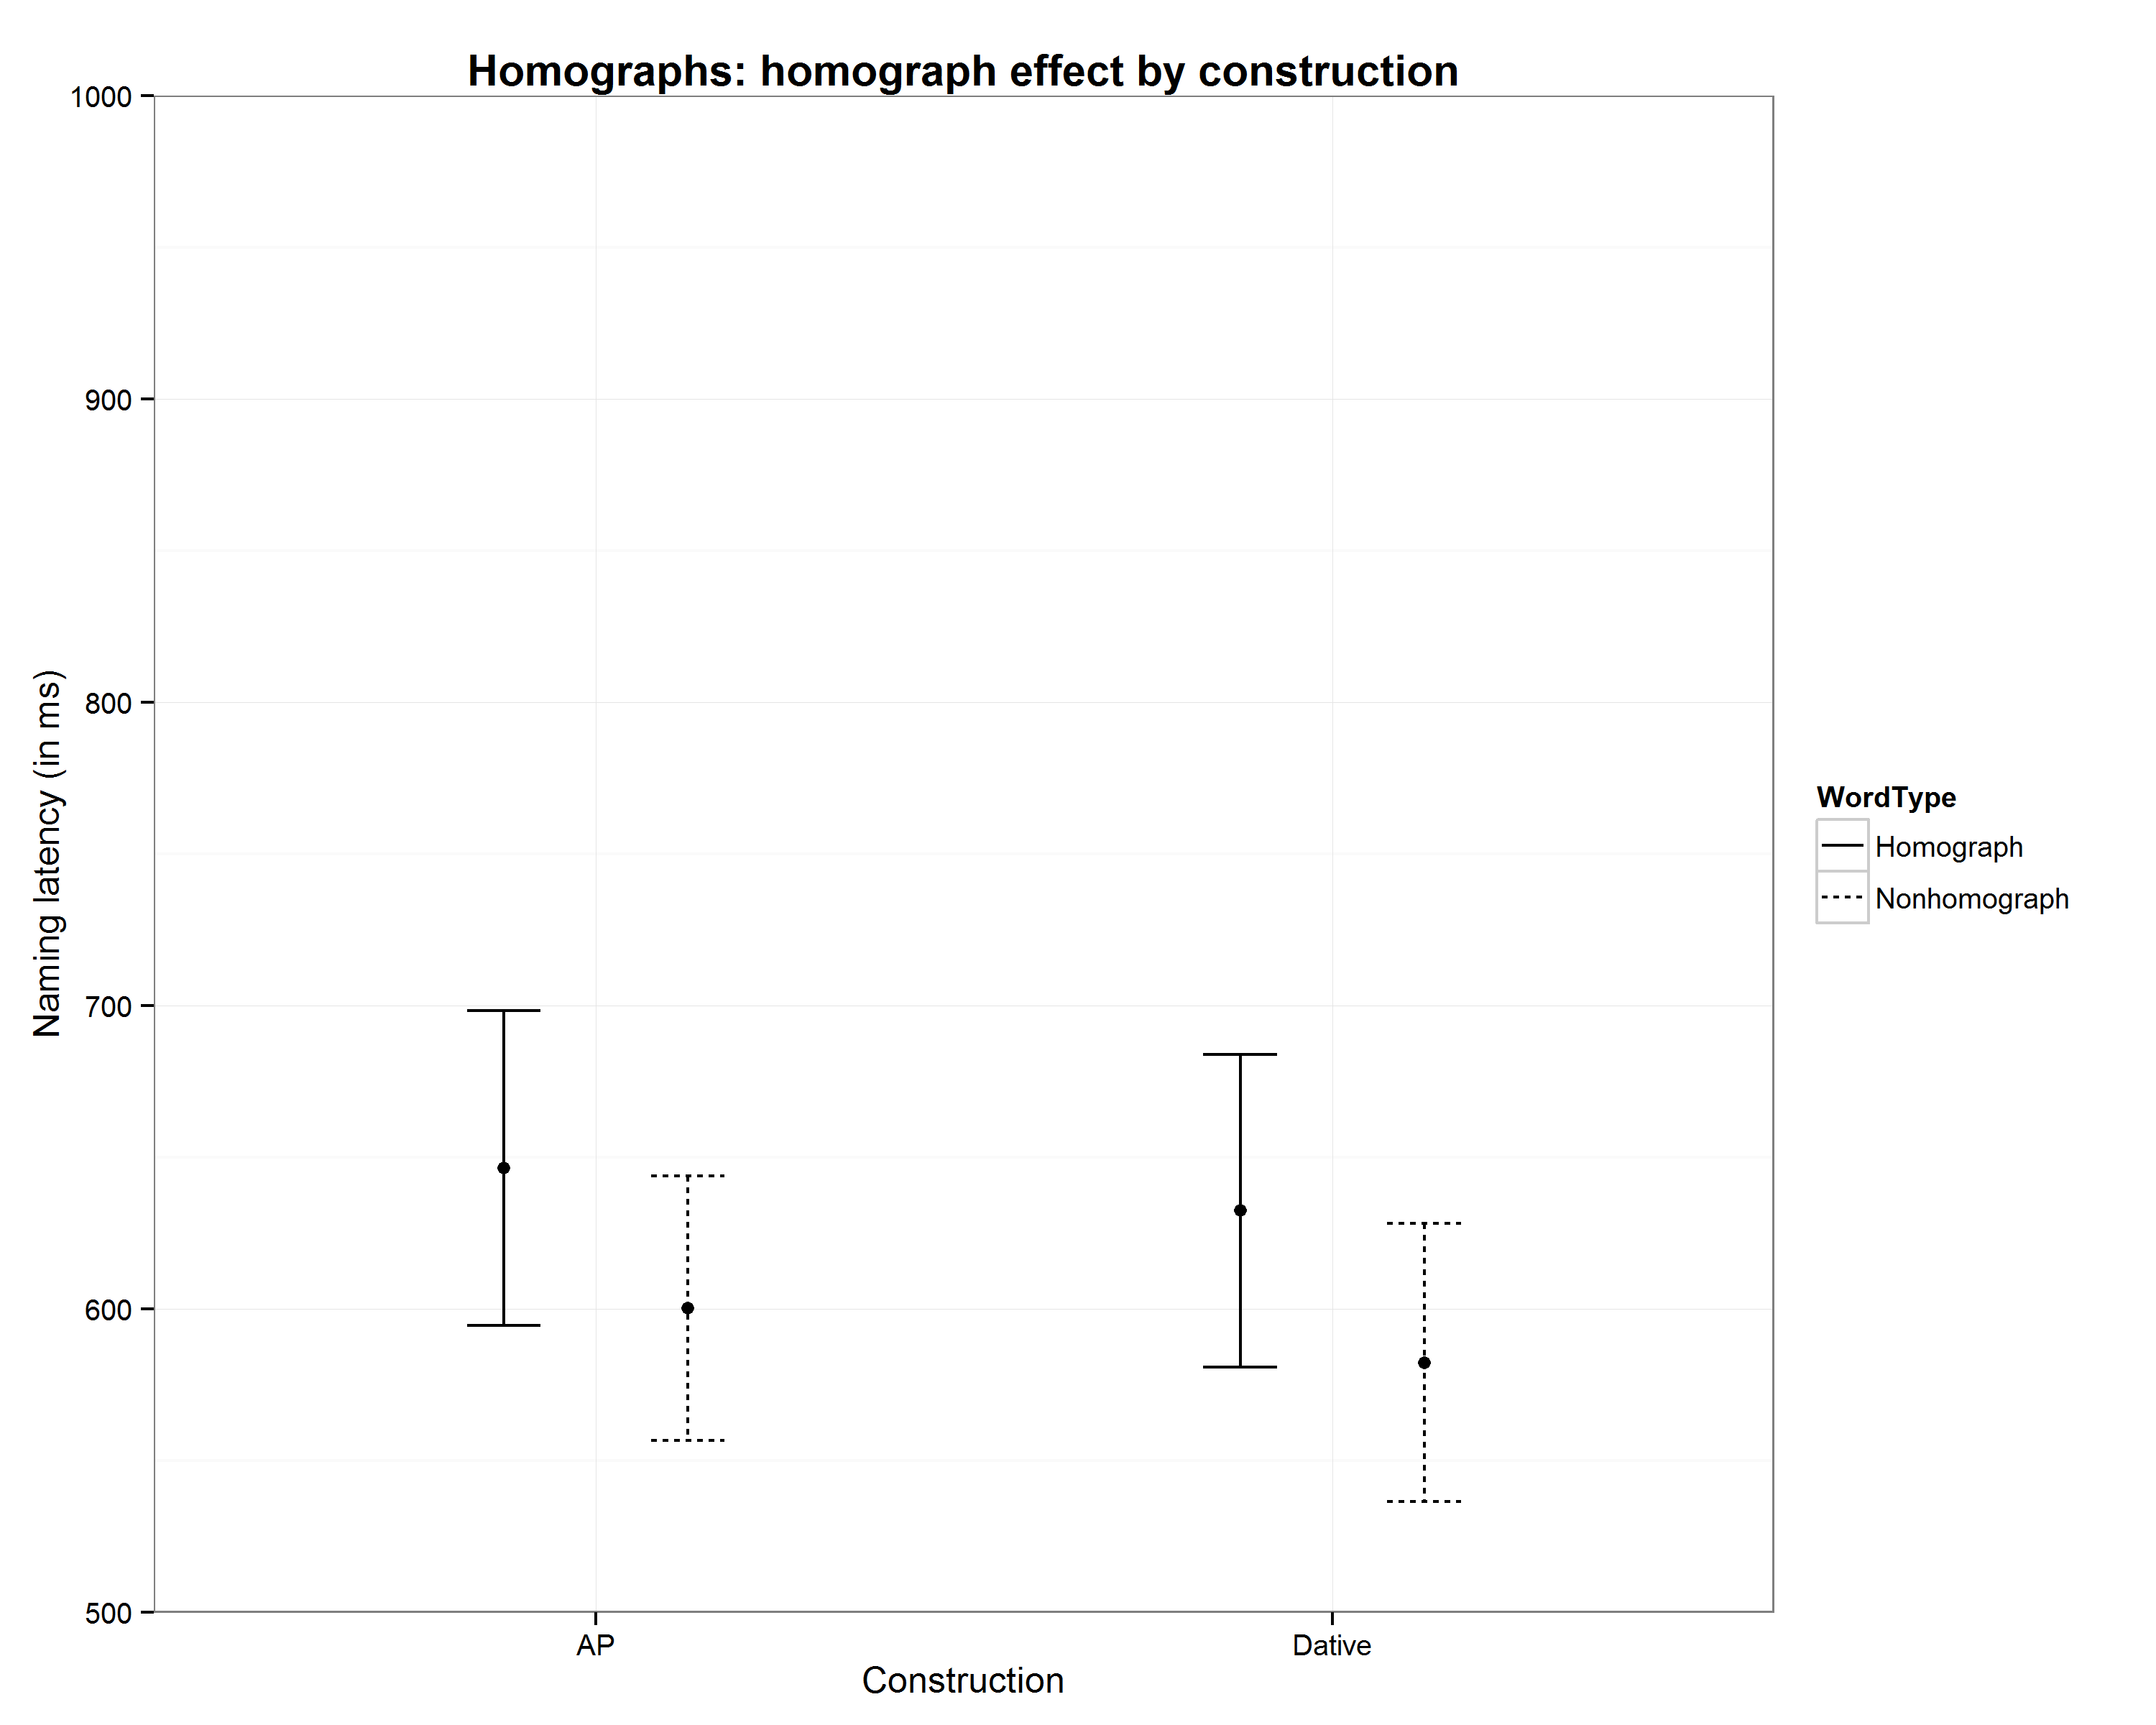
\includegraphics[width=\textwidth,height=\textheight,keepaspectratio]{conXwordtype-homs-excluded.png}
\caption{Plotted model fits for out-of-context homograph data after reanalysis in which item pairs that did not show homograph inhibition were excluded. Error bars depict 95\% confidence intervals.}
\label{fig:conXwordtype-homs-excluded}
\end{figure}


\begin{landscape}
% Table generated by Excel2LaTeX from sheet 'Sheet13'
\begin{table}[htbp]
  \centering
  \caption{Fixed-effects output for the cognate out-of-context reanalysis after  item pairs which did not produce cognate facilitation have been removed.}
    \begin{tabular}{rrrrrr}
    \toprule
          & Estimate & Std..Error & t.value & p.z   & Sig. \\
    \midrule
    (Intercept) & 6.422 & 0.033 & 196.396 & 0     & * \\
    clFrequency & -0.022 & 0.006 & -3.746 & 0     & * \\
    cLength & 0.022 & 0.004 & 6.21  & 0     & * \\
    WordType & -0.084 & 0.015 & -5.491 & 0     & * \\
    Construction & -0.007 & 0.014 & -0.459 & 0.646 &  \\
    WordType:Construction & 0.048 & 0.028 & 1.71  & 0.087 &  \\
    \bottomrule
    \end{tabular}%
  \label{tab:ocon.cog.reanl}%
\end{table}%



% Table generated by Excel2LaTeX from sheet 'Sheet14'
\begin{table}[htbp]
  \centering
  \caption{Fixed-effects output for the homograph out-of-context reanalysis after  item pairs which did not produce homograph inhibition have been removed.}
    \begin{tabular}{rrrrrr}
    \toprule
          & Estimate & Std..Error & t.value & p.z   & Sig. \\
    \midrule
    (Intercept) & 6.39  & 0.03  & 211.832 & 0     & * \\
    clFrequency & -0.047 & 0.009 & -5.161 & 0     & * \\
    cLength & 0.003 & 0.006 & 0.41  & 0.682 &  \\
    WordType & 0.072 & 0.02  & 3.714 & 0     & * \\
    Construction & 0.025 & 0.021 & 1.213 & 0.225 &  \\
    WordType:Construction & -0.01 & 0.04  & -0.248 & 0.804 &  \\
    \bottomrule
    \end{tabular}%
  \label{tab:ocon.hom.reanl}%
\end{table}%
\end{landscape}



\paragraph{Reanalysis of Experiment 2:\\ Spanish-English bilinguals in-context\\}
\label{reanalysisofexperiment2:spanish-englishbilingualsin-context}

The models from Experiment 2 were recomputed after calculating and removing item-specific cognate and homograph effects from Experiment 1. The results of the cognate model are as follows. There was an effect of Spanish picture naming composite, such that an increase in the composite (related to increased fluency in Spanish) related to a decrease in log RT (\emph{$\beta$} = --0.093, \emph{SE} = 0.023, \emph{t} = --3.997, \emph{p} $<$ 0.001). There was an effect of centered log word frequency, such that an increase in frequency related to a decrease in log RT (\emph{$\beta$} = --0.012, \emph{SE} = 0.005, \emph{t} = --2.459, \emph{p} $<$ 0.05). There was an effect of centered word length, such that an increase in number of characters related to an increase in log RT ($\beta$ = 0.014, \emph{SE} = 0.003, \emph{t} = 4.875, p $<$ 0.001). There was an effect for the contrast between passive and all other structures, such that words named in passive sentences were named more quickly compared to active sentences (\emph{$\beta$} = --0.011, \emph{SE} = 0.003, \emph{t} = --3.796, \emph{p} $<$ 0.001). There was no effect of the contrast between the two dative structures and active structure nor for the contrast between the two dative structures (\emph{t} $<$ 1, \emph{p}, $>$ 0.05). There was an effect for the cognate contrast such that, cognates were named more quickly compared to non-cognate controls (\emph{$\beta$} = 0.079, \emph{SE} = 0.019, \emph{t} = 4.202, \emph{p} $<$ 0.001). The cognate contrast interacted with Spanish picture naming composite, such that the magnitude of the cognate effect decreased with an increase in the composite (related to increasing Spanish fluency; \emph{$\beta$} = --0.047, \emph{SE} = 0.012, \emph{t} = --3.948, \emph{p} $<$ 0.001). The cognate contrast did not interact with any of the construction contrasts (\emph{t}s $<$ 1, \emph{p}s $>$ 0.05). There was no evidence for the addition of a three way interaction between Spanish composite, cognate contrast, and sentence structure in the model ($\chi^2$ (6) = 6.791, p = 0.34). See Table \ref{tab:incon.bil.cog.reanl} for the fixed-effects from the cognate model, and see Figure \ref{fig:Rplot38} for a partial effects plot. 

\begin{figure}[htbp]
\centering
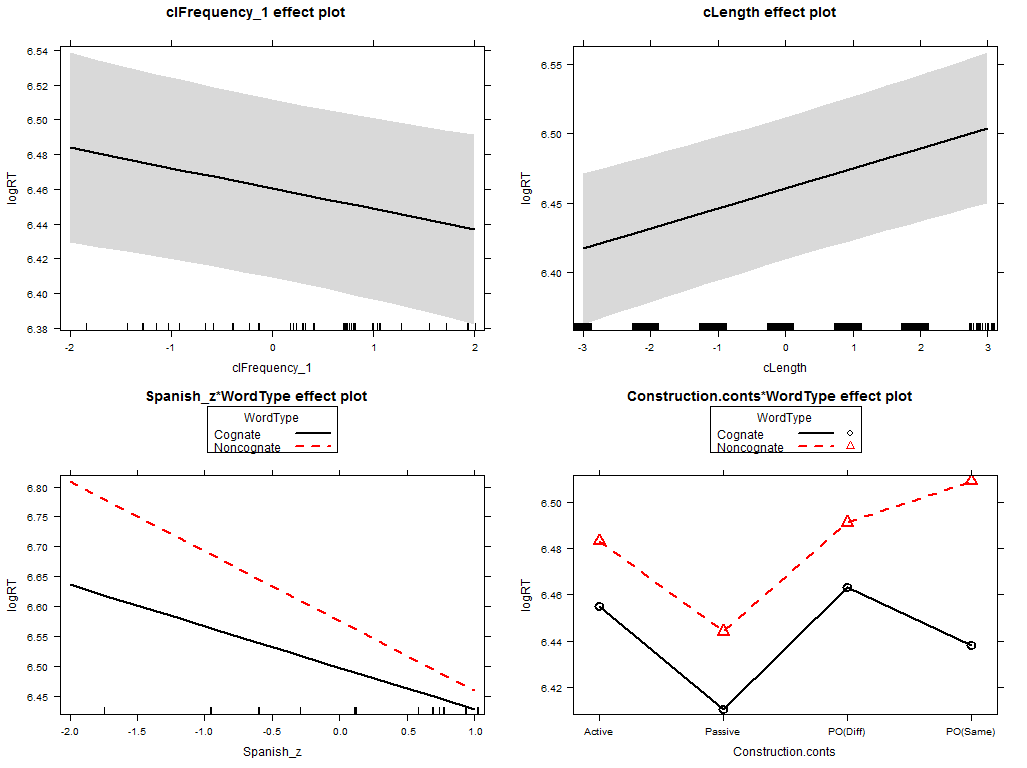
\includegraphics[width=\textwidth,height=\textheight,keepaspectratio]{Rplot38.png}
\caption{Plotted model fits for in-context cognate data after reanalysis in which out-of-context item pairs that did not show cognate facilitation were excluded. The y-axis is log reaction time. clFrequency\_1 is mean-centered log word frequency; cLength is mean-centered word length, Spanish\_z is the z-score Spanish fluency picture naming composite, and Construction.conts represents the different construction conditions. }
\label{fig:Rplot38}
\end{figure}


% Table generated by Excel2LaTeX from sheet 'Sheet15'
\begin{landscape}
\begin{table}[htbp]
  \centering
  \caption{Fixed-effects output for the cognate in-sentence-context reanalysis after item pairs which did not produce cognate facilitation out-of-context have been removed.}
    \begin{tabular}{rrrrrr}
    \toprule
          & Estimate & Std..Error & t.value & p.z   & Sig \\
    \midrule
    (Intercept) & 6.538 & 0.032 & 202.124 & 0     & * \\
    Construction.contsAll\_Act.V.Passive & -0.011 & 0.003 & -3.796 & 0     & * \\
    Construction.contsDats.V.Active & -0.002 & 0.005 & -0.442 & 0.658 &  \\
    Construction.contsNP-PP.V.PP-NP & 0.002 & 0.008 & 0.233 & 0.815 &  \\
    Spanish\_z & -0.093 & 0.023 & -3.997 & 0     & * \\
    WordTypeCog.V.Ncog & 0.079 & 0.019 & 4.202 & 0     & * \\
    clFrequency\_1 & -0.012 & 0.005 & -2.459 & 0.014 & * \\
    cLength & 0.014 & 0.003 & 4.875 & 0     & * \\
    Spanish\_z:WordTypeCog.V.Ncog & -0.047 & 0.012 & -3.948 & 0     & * \\
    Construction.contsAll\_Act.V.Passive:WordTypeCog.V.Ncog & -0.002 & 0.006 & -0.349 & 0.727 &  \\
    Construction.contsDats.V.Active:WordTypeCog.V.Ncog & -0.007 & 0.011 & -0.659 & 0.51  &  \\
    Construction.contsNP-PP.V.PP-NP:WordTypeCog.V.Ncog & -0.022 & 0.015 & -1.412 & 0.158 &  \\
    \bottomrule
    \end{tabular}%
  \label{tab:incon.bil.cog.reanl}%
\end{table}%
\end{landscape}

To explore possible interactions between cognitive control, language fluency, and language co-activation, we tested for higher-order interactions between cognitive control variables (AXCPT ratio of proactive control, OSpan z-score, and the Flanker effect z-score) and the cognate and construction contrasts, and between the Spanish picture naming composite and cognate and the construction contrasts. We evaluated significance for the interactions by model comparison to less complex models. This procedure resulted in the removal of 5 participants who did not have complete data on the tasks. There was a significant three-way interaction between z-scored OSpan score, the cognate contrasts, and the construction contrasts ($\chi^2$ (3) = 12.139, p $<$ 0.01). There was no three-way interaction between AXCPT reaction time ratio, the construction contrasts, and the cognate contrast; nor was there a two-way interaction between AXCPT ratio and the construction contrasts (\emph{p}s $>$ 0.05). There was, however, a significant interaction between the AXCPT ratio and the cognate contrast ($\chi^2$ (1) = 3.922, p $<$ 0.05). There was a significant three-way interaction between the Spanish picture naming composite, the construction contrasts, and the cognate contrast ($\chi^2$ (3) = 9.996, p $<$ 0.05). For the final model, random slopes by item were added for the centered AXCPT ratio and the o-span score.

In this new model. There was an effect of Spanish picture naming composite, such that an increase in the composite (related to increased fluency in Spanish) related to a decrease in log RT (\emph{$\beta$} = --0.087, \emph{SE} = 0.030, \emph{t} = --2.870, \emph{p} $<$ 0.01). There was an effect of centered log word frequency, such that an increase in frequency related to a decrease in log RT (\emph{$\beta$} = --0.014, \emph{SE} = 0.006, \emph{t} = --2.437, \emph{p} $<$ 0.05). There was an effect of centered word length, such that an increase in number of characters related to an increase in log RT ($\beta$ = 0.017, \emph{SE} = 0.004, \emph{t} = 4.668, p $<$ 0.001). There was no main effect of the AXCPT ratio measure nor of the z-score OSpan measure (\emph{t}s $<$ 1.96, \emph{p}s $>$ 0.05). There was an effect for the contrast between passive and all other structures, such that words named in passive sentences were named more quickly compared to active sentences (\emph{$\beta$} = --0.012, \emph{SE} = 0.005, \emph{t} = --2.548, \emph{p} $<$ 0.05). There was no effect of the contrast between the two dative structures and active structure nor for the contrast between the two dative structures (\emph{t} $<$ 1.96, \emph{p}, $>$ 0.05). There was an effect for the cognate contrast such that, cognates were named more quickly compared to non-cognate controls (\emph{$\beta$} = 0.071, \emph{SE} = 0.020, \emph{t} = 3.571, \emph{p} $<$ 0.001). The cognate contrast interacted the AXCPT ratio measure (\emph{$\beta$} = --0.032, \emph{SE} = 0.011, \emph{t} = --2.898, \emph{p} $<$ 0.01), indicating that a higher ratio score  ~\citep[reflective of greater pro-active cognitive control or reliance on contextual information; e.g.,][]{Braver2002} related to a smaller cognate effect. The cognate contrast interacted with Spanish picture naming composite, such that the magnitude of the cognate effect decreased with an increase in the composite (related to increasing Spanish fluency; \emph{$\beta$} = --0.041, \emph{SE} = 0.012, \emph{t} = --3.328, \emph{p} $<$ 0.01). The cognate contrast interacted with the contrast between the passive sentences and all other sentences, indicating that the cognate effect was smaller in the passive sentences (\emph{$\beta$} = --0.022, \emph{SE} = 0.010, \emph{t} = --2.200, \emph{p} $<$ 0.05). The other construction contrasts did not interact with the cognate contrast (\emph{t}s $<$ 1, \emph{p}s $>$ 0.05). The cognate contrast interacted with the z-score OSpan measure (\emph{$\beta$} = 0.033, \emph{SE} = 0.012, \emph{t} = 2.759, \emph{p} $<$ 0.01), indicating that cognate effects were facilitatory for participants with high span but inhibitory for participants with low span. None of the construction contrasts interacted with the Spanish picture naming composite nor did they interact with the z-score OSpan measure (\emph{t}s $<$ 1.96, \emph{p}s $>$ 0.05). However, there was a three-way interaction between the contrast of the two dative structures, the cognate contrast, and the z-score Ospan measure (\emph{$\beta$} = 0.034, \emph{SE} = 0.017, \emph{t} = 2.036, \emph{p} $<$ 0.05), indicating that the crossover interaction between O-Span and the cognate contrast was not present in the NP-PP dative sentences as compared with the PP-NP dative sentences. Finally there was a three-way interaction between the the contrast for passive structures compared to all other structures, the cognate contrast, and the Spanish picture naming composite (\emph{$\beta$} = 0.016, \emph{SE} = 0.007, \emph{t} = 2.419, \emph{p} $<$ 0.05), indicating that with higher fluency the cognate effect was reduced for all structures besides the passive. See Table \ref{tab:incon.bil.cog.reanl.exec} for the fixed-effects from the cognate model.
%% \begin{figure}[htbp]
%% \centering
%% 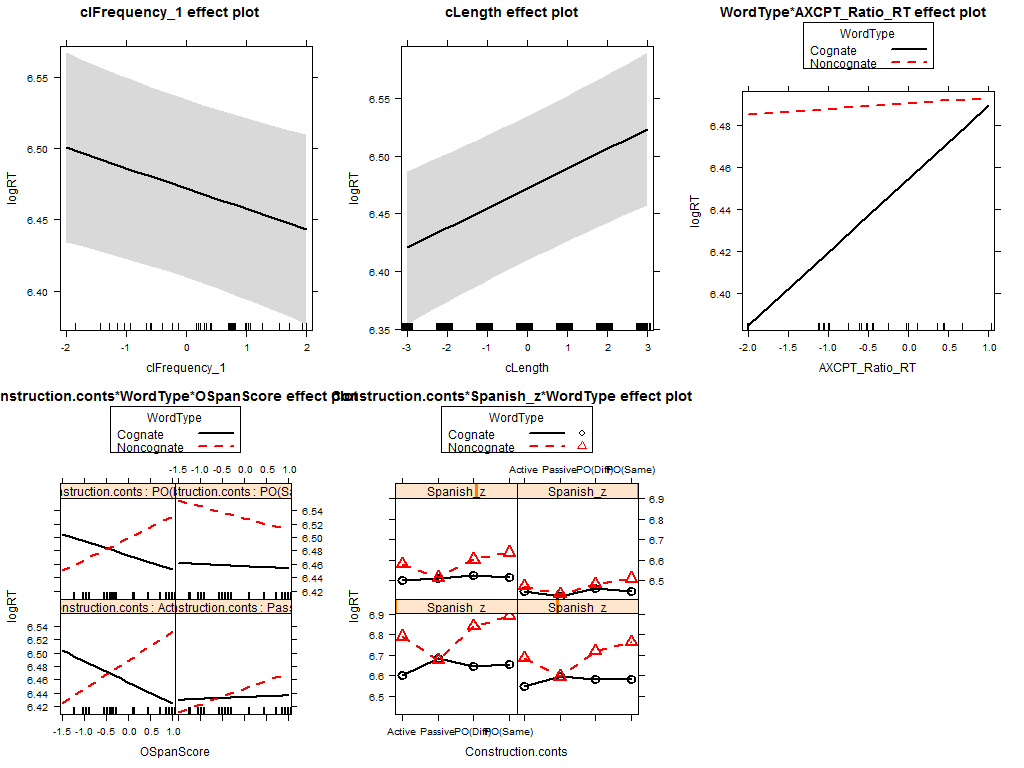
\includegraphics[width=\textwidth,height=\textheight,keepaspectratio]{Rplot40.png}
%% \caption{Plotted model fits for in-context cognate data after reanalysis in which out-of-context item pairs that did not show cognate facilitation were excluded. In this model, significant higher-order interactions with executive control variables and proficiency variables were included. The y-axis is log reaction time. clFrequency\_1 is mean-centered log word frequency, cLength is mean-centered word length, Spanish\_z is the z-score Spanish fluency picture naming composite, OSpanScore is the operation span score, AXCPT\_Ratio\_RT is the ratio value for the AXCPT task, and Construction.conts represents the different construction conditions. }
%% \label{fig:Rplot40}
%% \end{figure}


\begin{landscape}
  
% Table generated by Excel2LaTeX from sheet 'Sheet17'
\begin{table}[htbp]
  \centering
  \caption{Fixed-effects output for the cognate in-sentence-context reanalysis after item pairs which did not produce cognate facilitation out-of-context have been removed. In this model significant interactions with executive control have been included.}
\scalebox{0.7}{
  \begin{tabular}{rrrrrr}
    \toprule
          & Estimate & Std..Error & t.value & p.z   & Sig. \\
    \midrule
    (Intercept) & 6.548 & 0.041 & 160.386 & 0     & * \\
    Construction.contsAll\_Act.V.Passive & -0.012 & 0.005 & -2.548 & 0.011 & * \\
    Construction.contsDats.V.Active & -0.01 & 0.007 & -1.342 & 0.18  &  \\
    Construction.contsNP-PP.V.PP-NP & -0.007 & 0.012 & -0.575 & 0.565 &  \\
    Spanish\_z & -0.087 & 0.03  & -2.87 & 0.004 & * \\
    WordTypeCog.V.Ncog & 0.071 & 0.02  & 3.571 & 0     & * \\
    clFrequency\_1 & -0.014 & 0.006 & -2.437 & 0.015 & * \\
    cLength & 0.017 & 0.004 & 4.668 & 0     & * \\
    AXCPT\_Ratio\_RT & 0.019 & 0.031 & 0.608 & 0.543 &  \\
    OSpanScore & 0.004 & 0.034 & 0.104 & 0.917 &  \\
    Spanish\_z:WordTypeCog.V.Ncog & -0.041 & 0.012 & -3.329 & 0.001 & * \\
    WordTypeCog.V.Ncog:AXCPT\_Ratio\_RT & -0.032 & 0.011 & -2.898 & 0.004 & * \\
    Construction.contsAll\_Act.V.Passive:WordTypeCog.V.Ncog & -0.022 & 0.01  & -2.2  & 0.028 & * \\
    Construction.contsDats.V.Active:WordTypeCog.V.Ncog & -0.006 & 0.017 & -0.368 & 0.713 &  \\
    Construction.contsNP-PP.V.PP-NP:WordTypeCog.V.Ncog & -0.022 & 0.023 & -0.967 & 0.334 &  \\
    Construction.contsAll\_Act.V.Passive:OSpanScore & 0.003 & 0.003 & 1.05  & 0.294 &  \\
    Construction.contsDats.V.Active:OSpanScore & 0.003 & 0.004 & 0.592 & 0.554 &  \\
    Construction.contsNP-PP.V.PP-NP:OSpanScore & 0.008 & 0.008 & 0.985 & 0.325 &  \\
    WordTypeCog.V.Ncog:OSpanScore & 0.033 & 0.012 & 2.759 & 0.006 & * \\
    Construction.contsAll\_Act.V.Passive:Spanish\_z & 0.001 & 0.003 & 0.372 & 0.71  &  \\
    Construction.contsDats.V.Active:Spanish\_z & 0.005 & 0.005 & 1.068 & 0.285 &  \\
    Construction.contsNP-PP.V.PP-NP:Spanish\_z & 0.004 & 0.009 & 0.472 & 0.637 &  \\
    Construction.contsAll\_Act.V.Passive:WordTypeCog.V.Ncog:OSpanScore & -0.004 & 0.007 & -0.633 & 0.527 &  \\
    Construction.contsDats.V.Active:WordTypeCog.V.Ncog:OSpanScore & 0.018 & 0.011 & 1.706 & 0.088 &  \\
    Construction.contsNP-PP.V.PP-NP:WordTypeCog.V.Ncog:OSpanScore & 0.034 & 0.017 & 2.036 & 0.042 & * \\
    Construction.contsAll\_Act.V.Passive:Spanish\_z:WordTypeCog.V.Ncog & 0.016 & 0.007 & 2.419 & 0.016 & * \\
    Construction.contsDats.V.Active:Spanish\_z:WordTypeCog.V.Ncog & 0.001 & 0.011 & 0.117 & 0.907 &  \\
    Construction.contsNP-PP.V.PP-NP:Spanish\_z:WordTypeCog.V.Ncog & -0.001 & 0.017 & -0.053 & 0.958 &  \\
    \bottomrule
    \end{tabular}%
}
  \label{tab:incon.bil.cog.reanl.exec}%
\end{table}%
\end{landscape}


The results of the homograph model are as follows. There was an effect of Spanish picture naming composite, such that an increase in the composite (related to increased fluency in Spanish) related to a decrease in log RT (\emph{$\beta$} = --0.060, \emph{SE} = 0.024, \emph{t} = --2.508, \emph{p} $<$ 0.05). There was an effect of centered log word frequency, such that an increase in frequency related to a decrease in log RT (\emph{$\beta$} = --0.031, \emph{SE} = 0.006, \emph{t} = --4.946, \emph{p} $<$ 0.001). There no significant effect of centered word length (\emph{t} $<$ 1, \emph{p $>$} 0.05). There was an effect for the contrast between passive and all other structures, such that words named in passive sentences were named more quickly compared to active sentences (\emph{$\beta$} = --0.017, \emph{SE} = 0.005, \emph{t} = --3.438, \emph{p} $<$ 0.01). There was no effect of the contrast between the two dative structures and active structure nor for the contrast between the two dative structures (\emph{t} $<$ 1.96, \emph{p} $>$ 0.05). There was no effect for the homograph contrast, and no interaction between Spanish naming composite and the homograph contrast (\emph{t}s $<$ 1.96, \emph{p}s $>$ 0.05). However, the homograph contrast contrast interacted with the contrast between the active structure and the two dative structures, indicating that there was significant homograph inhibition in the dative structures (\emph{$\beta$} = --0.028, \emph{SE} = 0.013, \emph{t} = 2.215, \emph{p} $<$ 0.05). The homograph contrast did not interact with any other sentence construction contrast (\emph{t}s $<$ 1, \emph{p}s $>$ 0.05). The addition of an interaction term between construction and Spanish picture naming composite was significant via model comparison ($\chi^2$ (3) = 16.032, p $<$ 0.01), but the three-way interaction between construction, word type, and Spanish picture naming composite was not significant ($\chi^2$ (3) = 3.549, p = 0.31). The contrast between the passive and all other structures interacted with the Spanish picture naming composite (\emph{$\beta$} = 0.007, \emph{SE} = 0.003, \emph{t} = 2.160, \emph{p} $<$ 0.05), indicating that the speed-up for passive sentences became less dramatic with increased language fluency. The contrast between the two dative structures interacted with Spanish picture naming composite (\emph{$\beta$} = 0.019, \emph{SE} = 0.008, \emph{t} = 2.264, \emph{p} $<$ 0.05), indicating that a processing disadvantage arose for PP-NP structures at lower levels of proficiency. See Table \ref{tab:incon.bil.hom.reanl} for the fixed-effects from the homograph model, and see Figure \ref{fig:Rplot37} for a partial effects plot. 
\begin{figure}[htbp]
\centering
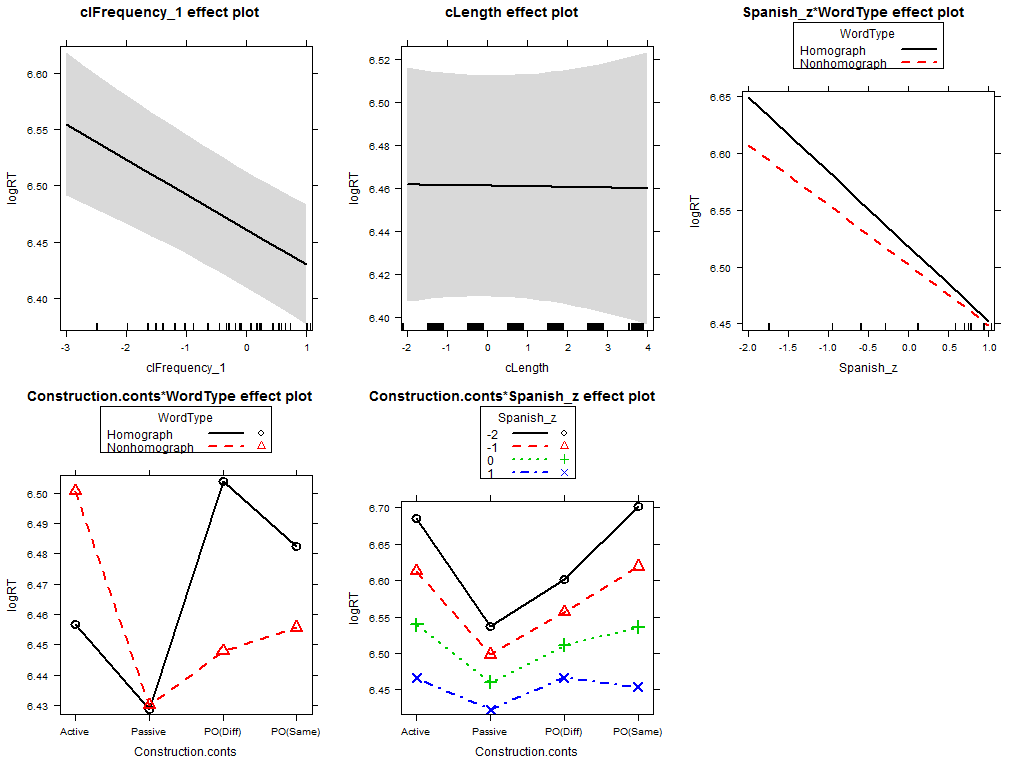
\includegraphics[width=\textwidth,height=\textheight,keepaspectratio]{Rplot37.png}
\caption{Plotted model fits for in-context homograph data after reanalysis in which out-of-context item pairs that did not show homograph inhibition were excluded. The y-axis is log reaction time. clFrequency\_1 is mean-centered log word frequency; cLength is mean-centered word length, Spanish\_z is the z-score Spanish fluency picture naming composite, and Construction.conts represents the different construction conditions.}
\label{fig:Rplot37}
\end{figure}


% Table generated by Excel2LaTeX from sheet 'Sheet16'
\begin{landscape}
\begin{table}[htbp]
  \centering
  \caption{Fixed-effects output for the homograph in-sentence-context reanalysis after item pairs which did not produce homograph inhibition out-of-context have been removed.}
    \begin{tabular}{rrrrrr}
    \toprule
          & Estimate & Std..Error & t.value & p.z   & Sig. \\
    \midrule
    (Intercept) & 6.512 & 0.033 & 198.777 & 0     & * \\
    Construction.contsAll\_Act.V.Passive & -0.017 & 0.005 & -3.438 & 0.001 & * \\
    Construction.contsDats.V.Active & 0.005 & 0.008 & 0.616 & 0.538 &  \\
    Construction.contsNP-PP.V.PP-NP & -0.012 & 0.011 & -1.051 & 0.293 &  \\
    Spanish\_z & -0.06 & 0.024 & -2.508 & 0.012 & * \\
    WordTypeHom.V.Ncog & -0.02 & 0.019 & -1.04 & 0.298 &  \\
    clFrequency\_1 & -0.031 & 0.006 & -4.946 & 0     & * \\
    cLength & 0     & 0.005 & -0.064 & 0.949 &  \\
    Spanish\_z:WordTypeHom.V.Ncog & 0.013 & 0.011 & 1.148 & 0.251 &  \\
    Construction.contsAll\_Act.V.Passive:WordTypeHom.V.Ncog & 0.004 & 0.007 & 0.515 & 0.606 &  \\
    Construction.contsDats.V.Active:WordTypeHom.V.Ncog & 0.028 & 0.013 & 2.215 & 0.027 & * \\
    Construction.contsNP-PP.V.PP-NP:WordTypeHom.V.Ncog & -0.015 & 0.019 & -0.753 & 0.452 &  \\
    Construction.contsAll\_Act.V.Passive:Spanish\_z & 0.007 & 0.003 & 2.16  & 0.031 & * \\
    Construction.contsDats.V.Active:Spanish\_z & -0.003 & 0.005 & -0.646 & 0.519 &  \\
    Construction.contsNP-PP.V.PP-NP:Spanish\_z & 0.019 & 0.008 & 2.264 & 0.024 & * \\
    \bottomrule
    \end{tabular}%
  \label{tab:incon.bil.hom.reanl}%
\end{table}%
\end{landscape}

To explore possible interactions between cognitive control, language fluency, and language co-activation, we tested for higher-order interactions between cognitive control variables (AXCPT ratio of proactive control, OSpan z-score, and the Flanker effect z-score) and the homograph and construction contrasts, and between the Spanish picture naming composite and homograph and the construction contrasts. We evaluated significance for the interactions by model comparison to less complex models. This procedure resulted in the removal of 5 participants who did not have complete data on the tasks. There was no evidence for higher order interactions between executive control variables, the homograph contrast, and sentence construction (\emph{p} $>$ 0.05 on all $\chi^2$ tests of model comparison).

\subsubsection{Discussion}
\label{discussion}

The Spanish-English bilinguals recruited for Experiment 2 showed evidence for the co-activation of English for Spanish target words embedded in Spanish sentence contexts. We observed significant cognate facilitation, the magnitude of which had an inverse relationship with L1 fluency. Bilinguals who were more fluent in their native language showed smaller cognate effects compared to bilinguals who were less fluent in their native language. We also observed a significant homograph effect, the magnitude of which was independent of L1 fluency. Critically, there was evidence that both cross-language effects depended on the syntactic context of the sentence. 

The magnitude of the cognate facilitation effect differed for the comparison between the two dative conditions. In the PP-NP condition the cognate effect was greatly reduced when compared to the NP-PP dative condition. Recall that the the PP-NP dative is predicted the be specific to Spanish on the account that the word order in the Spanish PP-NP sentence differs from its English translation, which must use either the double object dative (absent in Spanish) or the NP-PP dative. This suggests that the language-specific information encoded in the PP-NP dative condition may have allowed our sample of Spanish-English bilinguals to selectively access Spanish and ignore English. However, the follow-up analyses suggest that interaction is weak.

After we subset the items of the in-context study to include only the those that demonstrated a cognate facilitation effect outside of sentence context, the interaction between cognate status syntactic construction was no longer significant. On the one hand, this suggests that the interaction may have been due to confounded lexical factors. On the other hand, recall that the same cognate and matched control items were counterbalanced amongst the NP-PP and PP-NP dative conditions. As such, it is curious that the effect differed between conditions for this within-item comparison when all stimuli were included even if there were lexical confounds present for the dative items because the confounds are present to the same extent in NP-PP and PP-NP datives. One potential factor that may have shifted after the removal of the out-of-context items is orthographic similarity. The dative cognates that did not show an effect for bilingual speakers out-of-context (and were thus removed) were numerically higher in their orthographic similarity compared to the remaining cognates (M$_{Removed}$=.77, M$_{Not Removed}$=.67). Thus, the removed items should have shown a larger cognate effect, and indeed some did show a large effect of cognate inhibition out-of context which did not meet our criteria for inclusion. It is unclear yet how this influenced the results (further analyses are forthcoming), but one hypothesis is that by removing these items we diminished the overall cognate effect and reduced the likelihood of finding a significant interaction with syntactic construction. 

Like the cognate effect, the homograph effect also depended on syntactic construction, but unlike the cognate effect the interaction between the homograph effect and syntactic context was very robust. There was a facilitatory homograph effect in the active and passive constructions and an inhibitory effect in the dative constructions. The interaction was still significant when we conducted the more stringent analysis, including only homographs that showed an out-of-context effect. This suggests that the degree of language co-activation as measured by the homograph effect differed between active-passive sentences and dative sentences. The fact that the interaction was significant after the follow-up analysis with the subset of the most effective homograph and control pairs provides evidence that the difference between active-passive and dative sentences is not due to lexical confounds between conditions. Instead, the effect appears to be contextual. 

In a set of post-hoc analyses, we used model comparison to test for interactions between individual differences in executive function and language fluency and the predicted interaction between construction and word type. When the complete set of data was included, there were no higher order interactions between these variables. However, when we included only target words that showed a significant cognate or homograph effect in the out-of-context task, we found that participants' ability to exercise pro-active control was strongly related to the magnitude of the cognate effect, suggesting that participants with stronger proactive control over their two languages were able to reduce influence form the unintended language, when that influence might facilitate them. There was also evidence that the magnitude of cognate facilitation depended on working memory ability differentially between the two dative conditions and that the dependence of cognate facilitation on Spanish fluency was differential lessened in the passive construction compared to the other constructions. There were no such interactions for the homograph stimuli. These results, while preliminary, suggest that interactions between contextual variables and cognate effects are not always straightforward. Thus care must be taken when researchers fail to find an interaction between cognate effects and sentential context as they appear to co-depend in complicated ways with individual differences such as executive function and language proficiency. 

\section{General Discussion}
\label{generaldiscussion}

This study tested whether sentences that are hypothesized to contain Spanish-specific syntax can reduce co-activation of English in a combined visual word recognition and production task for a sample of highly proficient Spanish-English bilinguals. Spanish-English bilinguals co-activated both languages in an out-of-context word naming task, as evidenced by cognate facilitation. The magnitude of co-activation was not different for the two sets of homographs, one that was embedded in active and passive sentences and another that was embedded in datives in Experiment 2. There were no observable homograph effects, and no differences between the two sets. Monolingual speakers showed no differences between conditions for cognates and homographs, suggesting that the stimuli were well matched. In sentence context, a separate group of Spanish-English bilinguals also co-activated both languages. We observed cognate (facilitation) and homograph (facilitation and inhibition) effects during the production of target words that were embedded in Spanish sentences. Critically, the magnitudes of the cognate and homograph effects relied on the syntactic structure of the sentence in which the targets were embedded. Cognate effects were significant in all sentences, but were greater for dative sentences that shared word order between English and Spanish in comparison to dative sentences that had word order differences between the two languages. We hypothesize that dative structures are represented in a language-specific syntactic store ~\citep[e.g.,][]{Bernolet2007, Loebell2003} and that this language-specific storage could impact lexical access. The cognate modulation was weak, however; it depended on the set of items that were included in the analysis and was not significant when the set of items contained only those cognates and control pairs which demonstrated cognate facilitation in a separate out-of-context word naming task. In contrast, homograph effects robustly depended on the syntactic construction of the sentence, even when the subset of homograph-control pairs was restricted. Homograph effects were facilitatory in active and passive sentences, which contained word order overlap between English and Spanish, have been shown to prime across English and Spanish, and are hypothesized to be represented in language-non-specific syntactic stores ~\citep{Hartsuiker2004}. Furthermore, we found that cognate effects (but not homograph effects) depended on individual difference measures including fluency in the language of the task (Spanish, the L1), working memory span, and proactive inhibitory control. Cognate effects were generally smaller for individuals with greater pro-active control (i.e., those individuals who rely on contextual information) or for individuals with greater L1 fluency. The interactions between cross-language activation, syntactic context, and individual differences reported here are not predicted by the BIA+ model ~\citep{Dijkstra2002}, and a revised model should be considered.

Cognate and homograph effects are in line with many previous studies showing that bilinguals activate both languages when reading in one language alone, even when bilinguals read in the presence of context. Unilingual sentence contexts and tasks have been shown to be insufficient to restrict lexical activation to a single language ~\citep[e.g.,][]{Schwartz2006}, even when a direct comparison is made with mixed-language tasks ~\citep[e.g.,][]{Gullifer2013}. This is perhaps surprising. Throughout the course of an experiment entirely in one language, a reader could theoretically accumulate evidence supporting the single-language requirement and add it to their model of the situation to minimize influence of the unintended language. However, there was little evidence for this in the current data. Both languages were co-activated in parallel, and remained that way throughout the course of the task in the majority of sentence contexts. The results reported here extend the findings of previous studies in several ways by examining the factors which modulate cross-language co-activation, including the syntactic construction of the sentence and individual differences in language fluency and executive control.

\subsection{Influences of syntactic context}
\label{influencesofsyntacticcontext}

While many previous studies have investigated the role of potential language cues, e.g., language specific lexical form, aspects of contextual constraint, aspects of environmental constrain, aspects of task constraint, and semantic context ~\citep{Duyck2007, Gullifer2013, VanAssche2010,VanAssche2009, Pivneva2014, Lagrou2011, Libben2009, Schwartz2006, Titone2011}, it is curious that no published studies have investigated the role of syntax, a feature that differs wildly across languages, especially in realization the realization of the surface form (i.e., the linear word order within a sentence). Many of these previous studies report no interaction between cross-language effects and the so-called language cues ~\citep{VanAssche2010, Lagrou2011, Gullifer2013}. Here we show for the first time that syntactic context can function as a potential language cue. 

At the outset of the study, we hypothesized that the dative structures are represented in language-specific stores for Spanish-English bilinguals due to the presence of word order differences across the two languages, as suggested in the literature on cross-language syntactic priming ~\citep[e.g.,][]{Bernolet2007}. In contrast, active and passive structures share word order and have been shown to prime across languages for Spanish-English bilinguals ~\citep{Hartsuiker2004}, suggesting language non-specific representation. In the data reported here cognate effects appeared to be reduced in Spanish dative sentences that had a word order not licensed in English, and the direction of homograph effects changed from Spanish active and passive sentences (which have licit word order in English) and Spanish dative sentences (collapsed across the datives with shared word order and datives with language-specific word order). A reasonable interpretation of these two results is that the language-specificity of the dative sentences changed the degree to which a single language was required during sentence reading. When the specific activation of Spanish was triggered, it resulted in a decrease of English co-activation as measured by cognates. In the more stringent follow-up cognate analysis, For homographs, the effect did not simply become reduced following language-specific information. Instead, the effect became inhibitory in the dative sentences where the contrast between the two languages was highlighted through the presentation of language-specific syntactic information. Indeed,  \citet{Dijkstra1998} have argued that homograph inhibition is more likely to be observed when both languages are clearly present in the task and when responses must be language specific, as was the case in the present task in the dative conditions. 

The interaction between the cognate effect and syntactic construction was small and inconsistent, unlike that of the homograph data. The interaction between the cognate effect and the two dative constructions was no longer significant following an analysis on a more stringent subset of stimuli that may have been more sensitive to cross-language effects. This indicates that if there is a true interaction between cognate status and construction, it may be weak. The interaction between construction and the cognate effect was also inconsistent. In the more stringent analysis, the magnitude of the cognate effect was now reduced in passive sentences compared to all other sentences. In a way, passive sentences may also have language-specific properties when comparing Spanish and English that are not necessarily related to word order. Anecdotally, the passive construction in Spanish seems to be much less frequent, primarily occurring in writing. Spanish also has another variant of the passive construction that English does not have, the se-passive. Alternatively, the reduction in the magnitude of the cognate effect for passive sentences may simply related to the overall increase in speed in the condition, and a reduction in variability associated with fast responses, similar to the argument made in the bilingual semantic constraint literature ~\citep[e.g.,][]{VanAssche2010}. 

Small and inconsistent interactions between the cognate effect and syntactic construction are in line with unpublished results reported by  \citet{Gullifer2013}. They found that language-specific morphosyntactic features (the combined presence of pro-clitics and use of pro-drop in Spanish sentences, two features that are not present in English) did not, overall, impact the degree of non-selectivity as measured by the cognate effect. However, in a post-hoc analysis they reported the predicted interaction for a subset of speakers who were fastest on the task (which could have served as a proxy for language proficiency, though admittedly did not correlate clearly with any proficiency variables). In the present study, language proficiency was statistically controlled for, and the predicted interaction emerged. 

The results reported here are in line with word recognition studies showing that context can modulate activation of the unintended language ~\citep[e.g.,][]{Schwartz2006,Libben2009}. The primary factor that has been shown to be significant in modulating co-activation of the unintended languages is a strongly biased semantic context. When monolingual participants read a sentence, they generate predictions about upcoming words in that sentence. The predictions are particularly strong when a sentences is highly biased in its meaning. In highly biased sentences, the processing of upcoming words is speeded when they fit into the semantic frame and costly when they do not ~\citep{Duffy2001,Schwanenflugel1988}. For bilingual speakers, these predictions may also include information about the language membership of upcoming words, and this information in turn affects lexical processing. In addition to the general processing advantage for words that fit into a highly biased semantic frame, bilinguals experience a magnitude reduction for effects that are indicative of cross-language activation ~\citep{Schwartz2006}. The results here, suggest that language-specific syntax can function in a manner similar to that of to that biased of semantic context. Critically, the dative conditions did not exhibit a general speed-up or slowing of reaction time in comparison to other sentences (except the passive), eschewing an argument that has been made to discount the semantic constraint effect (the only other sentential effect that appears to reduce cross-language activation): that the drastic speed-up in recognition might mask otherwise observable cross-language effects. 

The evidence reported here that language-specific cues can reduce activation of the non-target language is in line with language-selective models of bilingual lexical access that assume bilinguals can use a selective attention mechanism perhaps guided by language-specific cues to alter the activation level of the non-target language ~\citep{Costa1999, Finkbeiner2006, LaHeij2005}. The syntactic context effects reported here are not explicitly predicted by the BIA+ model of word recognition. A strong version of the BIA+ model predicts that there should be no effects of linguistic context on word recognition. However, a weaker version predicts that any effects should occur late in processing. With the present data, it is impossible to explore the role of time-course, but future eye-tracking research could prove fruitful on this front. 

\subsection{Influences of language proficiency}
\label{influencesoflanguageproficiency}

The objective proficiency level in the language of the task (measured by a Spanish picture naming composite) determined the magnitude of the cognate effect. Individuals with higher Spanish fluency showed on average cognate effects with a smaller magnitude compared to less fluent bilinguals. In contrast, homograph effects were not related to language fluency. Both findings are consistent with those of  \citet{Pivneva2014} who showed that cognate facilitation (but not homograph inhibition) is dependent on L2 proficiency when the L2 was the language of the task. A straightforward interpretation of these results is that with increased language fluency, participants are better able to pre-activate the meaning of a word in the intended language, reducing the influence of the unintended language. However, our finding is somewhat surprising because fluency in the language of the task modulated cross-language co-activation but fluency in the second language did not and because the homograph effect was unrelated to language fluency. Thus, we entertain a potential alternative account of the cognate effect: that the cognate effect does not reflect language co-activation but is, rather, a relative frequency effect born out through the participants' knowledge of two languages. 

Because cognate share orthography, phonology, and meaning across two languages, a bilingual who speaks those two language necessarily will use these words more often compared to a monolingual speaker in either language. A well-known effect in the lexical processing literature (and one reported in the regression analyses here) is that words with higher frequency of usage will be processed, recalled, and named more quickly compared to words with lower frequency of usage ~\citep{Forster1973}. Thus, the bilingual cognate facilitation effect may be reflective of this increased frequency of usage, and the frequency effect is, in turn, is influenced by language fluency ~\citep{Gollan2008}. Homograph effects would not experience this same increased frequency of usage like the cognates because they differ in meaning, and as such will be used in different contexts across languages.

A counter-point to the frequency hypothesis is that, according to the hypothesis, only cognates with identical orthography across the two languages experience increased usage. Thus only identical cognates should experience cognate facilitation. However, contrary to this hypothesis, the magnitude of cognate facilitation has been shown to be related to the precise degree of orthographic overlap across the two languages. Words with greater orthographic overlap (including non-identical cognates) are processed faster compared to words with less overlap. This is indicative that the cognate facilitation effect is at least partially due to cross-language overlap. 

Still, the findings reported here and by ~\citep{Titone2011} are compatible with an account of cognate facilitation as a frequency effect. If cognate facilitation is truly a measure of language co-activation of the unintended language, then one would predict that the proficiency in the unintended language relate to the magnitude of cognate facilitation. A bilingual with a high proficiency in the unintended language should show the strongest cross-language effect, whereas a bilingual who is very weak in the unintended language should show little to no effect. However, neither here nor in the data of Titone and colleagues was this this case. Cognate facilitation was related to fluency in the language of the task at hand as opposed to fluency of the unintended language. Furthermore, data emerging from our lab suggests that native language cognate effects can occur very early in the learning of an L2. Second language learners who were enrolled in the first few semester of Spanish, showed evidence of processing English words that were cognates with Spanish differently compared to non-cognate control words ~\citep{Bice2013}. This is a finding that is consistent with a frequency interpretation of the cognate effect, and is less consistent with a parallel activation interpretation. If the cognate effect as a frequency effect hypothesis is correct, then it is unsurprising that the interaction with language-specific syntax is a weak effect as it does not track lexical co-activation.

\subsection{Influences of executive control}
\label{influencesofexecutivecontrol}

There were interactions between participants' individual differences in executive control and the magnitude of cross-language co-activation, specifically inhibitory control and working memory performance. Participants who exhibited better proactive inhibitory control, as measured by the AX- continuous performance task exhibited smaller magnitude cognate effects compared to participants with word proactive control. Proactive control is reflected in the ability to utilize contextual cues in AXCPT task to bias upcoming processing. In AXCPT participants respond strings of letters, and they respond ``yes'' to trials which fit a certain, highly frequent rule (press the yes key if the target is X that follows a previously displayed A). Participants with better proactive control are more likely to false alarm and hit yes when they see a non-X target character when it was preceded by the character A which strongly biases an X response. Here, apparently, participants with better proactive control were able to use contextual information regarding the monolingual nature of the task to eliminate activation of the unintended language. Good proactive control actually resulted in an increase in RT for cognate words (control words were relatively unaffected), presumably because participants who were proactively inhibiting the unintended language experienced surprisal when seeing the cognate words, which are licit words in the unintended language. Alternatively, perhaps the contextual awareness was related to the knowledge that there were homograph targets present, resulting in slower, more careful processing of the cognate words in proactive inhibitors. While  \citet{Pivneva2014} found no influence of executive control variables on cognate facilitation, a similar interaction between inhibitory control performance on the Simon task ~\citep{Simon1967} and the magnitude of the cognate effects has been shown during picture naming ~\citep{Linck2009}.

Participants' working memory span ~\citep{Unsworth2005} also appeared to correlate with the magnitude of the cognate effect across syntactic construction. Participants with a higher span tended to show cognate facilitation while participants with lower span tended to show cognate inhibition, except in the case of NP-PP dative sentences that share word order between English and Spanish. This suggests that a participants with higher working memory may have had less difficulty managing the multiple co-activated lexical representations compared to the lower span bilinguals. It is unexpected that this interaction disappears for the NP-PP sentences in relation to the PP-NP sentences. The NP-PP sentences share the most in common with the other sentences in terms of shared word order overlap. Furthermore, our cognate results suggest the NP-PP sentences may (marginally) allow for greater permeability between the two languages in comparison to the PP-NP sentences. Thus, the NP-PP condition should require greater executive control to manage the cross-language co-activation. Alternatively, the NP-PP sentences may represent a less cognitively demanding condition for the participant, requiring fewer cognitive resources thus eliminating the dependence, potentially by virtue of shared word order compared to the PP-NP condition. Though this does not explain why there the resources are again necessary in active and passive sentences, which also share word order between Spanish and English. While the result is unexpected, it begins to suggest that there are complicated higher order interactions between sentence context, executive function, and cross-language activation that have been relatively unexplored in the literature. A possible reason that other studies fail to observe interactions between cross-language effects and sentence context is that there are investigated higher order interactions masking the effects. 

Cross-language activation on the homograph trials was not related to either inhibitory control performance or working memory span. This is curious because homograph inhibition is thought to depend on participants ability to suppress the unintended meaning of the homograph distractor word and because other studies have found that executive control performance was related to homograph inhibition ~\citep[e.g.,][]{Pivneva2014}.

\subsection{Implications for models of word recognition}
\label{implicationsformodelsofwordrecognition}

The BIA+ model ~\citep{Dijkstra2002} was primarily designed to model single word recognition outside of sentence context. The model includes a word recognition system and a task schema. The word recognition system generally handles lexical activation while the task schema applies task decision criteria (e.g., response binding) to the output of the word recognition system. In this study, we found that the magnitude of parallel language co-activation depends on several factors: individual differences in fluency in the target language, individual differences in executive function, and the syntactic context of the sentence. Fluency and executive function variables interacted with the magnitude of the cognate effect, consistent with predictions of BIA+, but not the homograph effect, inconsistent with BIA+. Syntactic context interacted weakly with the magnitude of the cognate effect but strongly with the magnitude of the homograph effect; both interactions are inconsistent with BIA+. It is unclear, in terms of the BIA+ model, why the homograph effect failed to interact with fluency and executive function. Perhaps the failed interaction arose because the sentence context was a stronger modulating cue for homographs, whereas for cognates, the stronger modulating factor consisted of individual difference variables. 

The interaction between cross-language activation as measured by the cognate effect and proficiency in the target language is generally consistent with BIA+. Increasing the target language fluency within the model (plausibly through raising the baseline activation levels of the target language) would cause lexical representations of the target language to be activated more quickly increasing the speed of lexical access independent of word class. While cognates are still activated faster than controls, at some point for the highest fluency levels, the activation will occur so quickly that both cognates and control are speeded until they reach a floor in response time, effectively eliminating the cognate advantage and giving rise to the interaction between cognate effect and fluency. It is not entirely clear, however, why the homographs do not experience a similar dependence on language fluency if the same principles are in effect for both sets of words. 

The interaction with executive control is also generally consistent with BIA+ if we assume that the interaction occurs post-lexically during the decision process in the task schema. Following lexical activation in the word recognition system (in which both languages become co-activated), the model applies decision criteria (i.e., speak the word in Spanish) to this output from the word recognition system. At this point, the lexical alternative in the intended language must be selected so that the word can be correctly spoken. Apparently, executive function variables can alter the speed of this process differentially for cognate and control words. Higher proactive inhibitory control actually impedes the decision process for cognate words because the cognate (which is a licit word in the unintended language and which would normally experience speeded lexical access) actually becomes inhibited by good proactive control (i.e., attention to the single language contextual aspect of the task). Thus, the model might struggle with cognate words for low values of operation span when, at the level of the task schema, it must manage the multiply co-activated alternatives of the cognate. While the interactions between executive function and cross language activation are consistent with BIA+ if they occur at late stages of recognition, they are inconsistent if they occur at early stage. While the results here cannot provide insight about the time-course of the interactions, some recent eye-tracking research has shown that executive function variables do interact with language co-activation from the earliest points of processing, inconsistent BIA+ model ~\citep{Pivneva2014}. To the extent that our results are comparable with those of  \citet{Pivneva2014}, a revised version of the BIA+ should be considered that incorporates an executive control component within the word recognition system, or that allows the task schema to influence word recognition.

Because BIA+ was designed to account for word recognition in isolation form sentence context, it predicts that word recognition in the context of sentence reading should function almost identically to that of word recognition outside of sentence context. For the most part the extant empirical findings are consistent with this prediction ~\citep[e.g.,][]{VanAssche2010}: both languages become activated at early stages of recognition and remain activated into late stages of word recognition, despite the presence of a sentence context that could potentially provide cues about the language membership of upcoming words in a sentence. However, here we report the first evidence that the syntactic context in which a target word was embedded influenced the magnitude of cross-language activation, weakly for cognates and robustly for homographs, against predictions of BIA+. BIA+ currently has no way to incorporate syntactic context within the model. If we assume the syntactic interaction influences co-activation at a late stage in recognition ~\citep[consistent with other findings of interactions between sentence context and cross-language activation e.g.,][]{Libben2009}, the syntactic information might then come to encourage language-general response or a language-specific response at the level of the task schema ~\citep[see e.g.,][]{Dijkstra1998}.

For example, the presence of the dative construction, which does not share word order between English and Spanish and which could provide a language-specific cue as to the language membership of the currently activated word, might trigger a strong language-specific response at the level of the task schema, resulting in an inhibitory homograph effect in the dative conditions. In contrast the active and passive conditions, which share word order and are likely represented in language non-specific syntactic stores, trigger a language-general response resulting in homograph facilitation. A counter argument is that, presumably, the requirement to speak a word in a particular language should already necessitate a language-specific response. However, work on bilingual language production has begun to show that both languages can remain co-active quite late in processing, even the the point of articulation ~\citep{Jacobs2005} when this single-language requirement is present, suggesting that the requirement to speak in one language may not be language-specific enough. Thus for language-general response triggered by active and passive conditions, both languages could remain co-activated during articulation, whereas for language-specific response triggered by dative conditions, selection occurs  relatively earlier. 

Finally, the relatively stronger interaction between syntactic context and homographs and the relatively weaker interaction with cognates could reconcile the inconsistencies in the observation of interactions between language fluency and executive control for cognates, but not for homographs. If, in a revised BIA+ model, syntactic context were allowed to function as a language cue (potentially early on in word recognition), then it might reduce the need for executive function because the target language is specified by the context. Similarly, the syntactic interactions may mask or reduce the interactions between language fluency and cross-language activation for the homographs. In contrast, because the cognates are more likely to remain activated despite the presence of a potentially informative syntactic context, executive function and fluency variables are open to interact with cross-language co-activation. 

\section{Conclusion}
\label{conclusion}

To conclude, we found that language proficiency, executive control, and aspects of sentence context all play roles in determining the extent to which two language interact during bilingual word recognition. Our findings are consistent with a blossoming literature on bilingual language control showing that bilinguals experience constant co-activation of the two languages and that they must employ cognitive mechanisms to reign in this co-activation. We show, perhaps for the first time, that bilinguals can also use language-specific aspects of sentence context, here the syntax that differs in word order between two languages, as an additional means to control language co-activation. There also a suggestion in the findings that the two loci of control, executive function and aspects of the sentence context, function in a mutually exclusive manner: where there was evidence for interactions between sentence context and the degree of language co-activation, there was little evidence for the influence of executive control ability. However, future research will be necessary to validate this suggestion. Finally, information regarding the precise time-course of the reported effects will be critical in determining whether models of bilingual word recognition need to be revised. The BIA+ model predicts that the reported context effects should occur late in the time-course of processing; our word naming measure, while it provides a good first step in investing the role of context in word recognition, only probes the end-point of the comprehension-production process. As such we cannot determined from the present data how early in the word recognition process the contextual constraints took effect. Methodologies such eye-tracking and ERP are the next step in determining the time-course of the time-course of the reported effects and whether the BIA+ model should be updated. 

%% \begin{landscape}
%% \section{Tables and Figures}
%% % Table generated by Excel2LaTeX from sheet 'Sheet6'

\clearpage





\clearpage





\clearpage




\clearpage





\clearpage




\clearpage








\clearpage





\clearpage





\clearpage



%% 


\clearpage



\clearpage


%% \end{landscape}


\chapter{Representation of bilingual\\ syntax: The role of word order}
\label{representationofbilingualsyntax:theroleofwordorder}

\section{Introduction}
\label{introduction}

When bilinguals speak or read in one language, they co-activate information in both of the languages. Most research on cross-language activation (or language non-selectivity) has been conducted at the lexical level and has examined both production or comprehension. Lexical and lexicosemantic information about the unintended language becomes activated early in processing ~\citep{Duyck2007} and stays active for an extended period of time even into articulation ~\citep{Jacobs2005}, suggesting that this information is shared between the two languages ~\citep[e.g.,][]{Dijkstra2005, Kroll2013}. Cross-linguistic differences do not seem to play a strong role in modulating co-activation. Lexical co-activation is observed despite differences in orthography or phonology between the two languages ~\citep[e.g.,][]{Thierry2007}. A key question is how bilinguals reign in the activation from the unintended language and focus attention on the intended language. This control is crucial in production, where the lack of language selection would result in the catastrophic inability to speak. One proposal is that bilinguals exercise cognitive control to select the intended language and suppress or inhibit the unintended language ~\citep{Abutalebi2007,Green2013}. During comprehension there are relatively few constraints on cross-language activation, in some cases the languages remain co-activated without an overt language selection ~\citep{Duyck2007,VanAssche2010}. A growing literature is showing that bilinguals also co-activate syntactic representations across the two languages, and a question of interest is what factors, if any, modulate co-activation at this level ~\citep{Hartsuiker2004,Bernolet2007}. The factor explored here is linear word order overlap.

The primary methodology used to study co-activation at the syntactic level is cross-language syntactic priming. Classically, syntactic priming is the empirical observation that (monolingual) speakers tend to reuse syntactic structures that they have heard recently. For example, when English speaking participants read aloud a prime sentence that contains the active or passive voice (e.g., active: ``The lightning struck the house'' or passive: ``The house was struck by lightning'') and are then asked to describe a picture of a novel event (e.g., a man eating an apple), participants are more likely to describe the picture using the passive voice when the preceding sentence uses the passive voice ~\citep{Bock1986}. While repetition of words between the prime and the target can provide a lexical boost, increasing the rate of syntactic priming, it is not a necessary condition. This indicates that it is the abstract, underlying structure of the sentence that is primed and not simply lexical aspects of the prime sentence that are repeated. 

Since  \citet{Bock1986}, syntactic priming and its cross-language variant have been shown using many different production and comprehension tasks. Perhaps the quintessential syntactic priming production task is the picture-description\\ paradigm. Here, a participant is exposed to prime sentences under the guise of a cover task and is then asked to produce descriptions of novel pictures unrelated to the prime sentences ~\citep{Chen2013}. Sometimes the participant is asked to read sentences aloud and sometimes they are exposed to the prime sentences auditorily. Often a cover task is given to distract the participants from the goal of the study. For example participants will be told that a memory test will follow the task where they are asked to remember the pictures and sentences, or they will be asked to detect repetitions in the stimuli. Another variant of the picture description task involves a confederate participant. In this variant the two ``participants'' take turns describing pictures to one another. While the na\"{i}ve participant generates descriptions, the confederate reads prime sentences from a script ~\citep{Bernolet2010, Bernolet2013, Chen2013, Hartsuiker2004}. Other production tasks involve sentence recall ~\citep{Meijer2003, Potter1998, Shin2009}, in which participants read and remember a sentence, see an intervening prime sentence, and then recall the original sentence; and sentence completion, where participants hear or read incomplete sentences (including prime and probe sentences) are complete them verbally or in writing ~\citep{Branigan2000,Desmet2006, Pickering1998, Hatzidaki2011, Salamoura2007}. Syntactic priming has also been observed in naturalistic tasks including corpus research ~\citep{Cacoullos2010,Gries2005, Jaeger2007, Szmrecsanyi2006,Travis}. In all of the production tasks, the dependent measure of interest is essentially the likelihood of repetition of a given structure. 

Syntactic priming also occurs during language comprehension ~\citep{Arai2007, Branigan2005, Ledoux2007, Noppeney2004, Traxler2008, Thothathiri2008}. Reading or hearing a prime sentence with a particular structure enhances later comprehension of that structure, and has been shown to impact predictive eye-movements ~\citep{Arai2007, Thothathiri2008, Traxler2008}, to alter interpretation of syntactically ambiguous sentences ~\citep{Branigan2005}, and to reduce difficulty of syntactic integration as measured by event-related potentials ~\citep{Ledoux2007}, self-paced reading, and eye-tracking ~\citep{Traxler2008}. While relatively task independent, the detection of syntactic priming is more subtle in comprehension tasks such as self-paced reading where lexical repetition is often required to obtain a significant effect ~\citep[e.g., ][]{Ledoux2007, Thothathiri2008}. There are a small number of comparisons between methodologies ~\citep[see e.g., ][]{Chen2013, Tooley2009}, and no published studies, to my knowledge, that compare priming across modality. 

For bilingual speakers syntactic, priming occurs across languages. The cross-language permeability indicates that structural representations are shared between the two languages.  \citet{Loebell2003} showed that German (L1) -- English (L2) bilinguals exhibited cross-language priming for structures in the dative alternation (e.g., double object: The boy sent his pen pal a letter [Der Junge schickte seinem Breiffreund einen Brief]; prepositional dative: The boy sent a letter to his pen pal. [Der Junge schickte einen Brief an seinen Brieffreund]). Similar findings have been shown for the dative alternation in Dutch-English bilinguals~\citep{Schoonbaert2007}, Swedish-English bilinguals ~\citep{Kantola2011}, and Greek-English bilinguals ~\citep{Salamoura2007}; the adjective-noun\slash relative clause alternation in Dutch and German ~\citep{Bernolet2007}; as well as with the active\slash passive alternation in Spanish-English bilinguals ~\citep{Hartsuiker2004} and Polish-English bilinguals ~\citep{Fleischer2012}. 

Cross-language syntactic priming occurs bi-directionally across the two languages, suggesting that both languages draw from an integrated, language non-specific syntactic store. The effect has been observed primarily from L2 to L1 ~\citep{Desmet2006, Hartsuiker2004, Meijer2003, Salamoura2007}, L1 to L2 ~\citep[e.g.,][]{Bernolet2013}, and bi-directionally ~\citep{Bernolet2007, Kantola2011, Loebell2003, Schoonbaert2007, Shin2009, Weber2009}. Few studies, however, directly investigate the role of language proficiency in shaping the magnitude of cross-language priming, but the extant work suggests that lower proficiency bilinguals demonstrate a smaller degree of priming in comparison to high proficiency bilinguals. This indicates that at lower levels of proficiency, the two languages may depend on separate syntactic representations that merge as language proficiency increases ~\citep{Bernolet2013}. 

There are two general theoretical accounts of syntactic priming. One mechanism, transient activation ~\citep[e.g.,][]{Collins1975}, states that priming is the result of temporary activation of syntactic categories. After hearing a prime sentence in passive voice, for example, a participant's activation level of the passive construction is heightened. Thus, on the next trial the passive will be relatively more available for selection as compared to previous trials, and the passive will be more likely to be uttered. A second account of syntactic priming is implicit learning ~\citep{Bock2000, Bock2007, Chang2006}. In this account, participants learn throughout their experience with and exposure to abstract procedural knowledge ~\citep[e.g.,][]{Seger1994}, here, syntactic structures. In this account, hearing a prime sentence causes a long-term change to the system, something that is not predicted by the transient activation mechanism. Indeed, researchers have found long-term effects of syntactic priming ~\citep[e.g.,][]{Bock2000}. There are also hybrid accounts, that attempt to bridge the two mechanisms ~\citep[e.g.,][]{Hartsuiker2008, Reitter2011}. Crucially, the two primary accounts of syntactic priming make different predictions about the time-course of priming effects. In an activation account, the activation level eventually decays. Thus, priming is a relatively short-term process and one that should be consistent across the time-course of a task. In contrast, implicit learning predicts priming can be long term. Thus, the use of a primed structure may build up over the course of repeated exposure.

\subsection{The role of word order overlap}
\label{theroleofwordorderoverlap}

While the proposal in the literature has been that bilinguals have shared syntactic storage, most studies on cross-language syntactic priming only investigate structures that share word order between the two languages. Yet, monolingual studies on syntactic priming have found that word order is an important factor ~\citep{Hartsuiker1999, Hartsuiker2000, Pickering2002}; speakers tend to reuse the word order that was heard in a prime sentence. Work from the domain of code-switching shows that bilingual speakers are also sensitive to word order differences between the two languages. Code-switching is a phenomenon whereby some bilinguals intermix their two languages when speaking with other, similar types of bilinguals. Code-switching can occur mid-sentence (i.e., intrasentential switching), and the choice point of where to switch languages within a sentence is governed by word order constraints. Corpus studies of naturalistic speech show that speakers are less likely to switch languages at a point in a sentence where the word order is not equivalent between the two languages, and often this type of switch is considered ungrammatical ~\citep{Poplack1980, Lipski1978}. Likewise, experimental work on code-switching and word order preferences indicates that bilinguals prefer to switch languages when word order is shared but will also align with their dialog partner in their choice of word order and code-switching behavior ~\citep{Kootstra2010}. Taken together, these results suggest that word order differences may play an important role in differentiating structural representations between two languages, and priming provides the perfect test-bed to investigate these differences in representation.

Cross-language syntactic priming is relatively robust for structures that overlap in word order. While  \citet{Loebell2003} observed cross-language priming for dative structures between German and English (which overlap in their word order across languages), they observed no such priming for active and passive sentences (active: The janitor cleans the floors daily [Der Hausmeister reinigt die B\"{o}den t\"{a}glich]; passive: The floors are cleaned daily by the janitor [Die B\"{o}den werden t\"{a}glich von dem Hausmeister gereinigt [literally: ``The floors are daily by the janitor cleaned'']. They speculated that the lack of priming was due to the lack in word order overlap between German and English. In this alternation, the passive structure differs in word order across the two languages because the main verb of the German sentence (``gereinigt'' the past participle of the verb to clean) comes at the end of the clause. In line with this hypothesis, the active-passive alternation has been shown to prime between other languages where the word order overlaps (e.g., Spanish and English). Similar word order dependent results have been shown in the adjective-noun\slash relative clause alternation in German and English. Relative clauses in German exhibit verb-final structure in contrast to English and this structure does not elicit priming ~\citep{Bernolet2007} and prepositional object dative constructions that involved word order variations between Greek and English ~\citep{Salamoura2007}. Taken together, these results suggest that bilingual speaker may have language-specific syntactic representations for some structures, and that this specificity depends on word order overlap. Crucially, bilinguals are capable of learning and processing the syntactic structure in their L2 indicating that the lack of priming is not due to failed acquisition or shallow processing of a structure.  \citet{Flett2012} showed that Spanish-English bilinguals exhibit within-language priming for dative structures in their L2 despite the lack of word order overlap, indicating that they can access this structure in the L2. 

There are cases in which priming is observable across languages despite the presence of word order differences. Relative clause attachment sites (e.g., NP1 vs. NP2 attachment) have been primed across Dutch and English despite Dutch a verb-final structure for relative clauses ~\citep{Desmet2006}. Priming between the dative alternation has been observed for Korean-English bilinguals despite the fact that Korean and English differ in typological word order ~\citep[Korean has SOV word order while English has SVO word order;][]{Shin2009}.  \citet{Weber2009} found priming of the passive structures in English that did not differ depending on whether the prime was in German or in English, suggesting that the German passive could prime the English passive ~\citep[in contrast to][]{Loebell2003}. However, the study was perhaps underpowered (N=15) to detect a significant interaction between prime structure and language. Finally,  \citet{Fleischer2012} found the Polish active OVS structure primed use of the English passive in Polish-English bilinguals. In one sense, this result suggests that priming can occur despite word order differences between languages because English does not have OVS word order in active sentences. However, the results stress the importance of linear word order because participants were primed to produce a construction (the English passive) in which the linear order of thematic roles overlapped across languages ~\citep[the passive and OVS both place stress on the grammatical patient by fronting it; see also][]{Loncke2011} who primed attachment resolution of a complex noun phrase across dissimilar syntactic structures). Clearly, the distinction between shared and separate syntactic representations as dictated by the presence or absence of word order differences is not clear-cut. However, the presence of discrepancies in the results of experiments utilizing structures with word order differences across languages suggests that the degree of representational overlap is reduced when word order is not shared.

An alternative explanation for the discrepancy in the studies presented above regarding priming and word order differences is that the results are confounded with the type of task being used. Studies that find an asymmetry in priming between overlapping and non-overlapping word order tend to use the classical picture priming paradigm in which confederate speakers present participants with prime sentences before the participants describe a scene ~\citep{Bernolet2007, Loebell2003} or other production oriented experiments ~\citep{Salamoura2007}. In contrast, the studies finding evidence for cross-language syntactic priming despite word order differences have used a wider range of tasks including sentence recall and self-paced reading. There may therefore be differential sensitivity across tasks to detect cross language priming for structures without word order overlap. Comprehension tasks, such as self-paced reading, tend to be less sensitive to the detection of syntactic priming ~\citep{Ledoux2007, Thothathiri2008} and typically require lexical repetition to obtain priming. 

\subsection{The present study}
\label{thepresentstudy}

The goal of the present study is to determine the extent to which Spanish-English bilinguals share representations for syntactic structures using syntactic priming. Previous syntactic priming studies on Spanish-English bilinguals have found that there is significant cross-language priming for Spanish-English bilinguals with active and passive structures ~\citep{Flett2003,Hartsuiker2004} and with prepositional object dative structures ~\citep{Flett2013,Meijer2003}, indicating that those structures may share representations across the two languages. Thus far, each of these tested structures have shared word order between English and Spanish, including the prepositional object dative sentences, which can optionally differ in word order between the two languages. Spanish, but not English, freely allows for PP-NP datives (e.g., Un hombre mostrando a una mujer su celular [A man showing to a woman his phone]). However, no studies have tested whether such word order differences allow for distinct representations for Spanish-English bilinguals. 

To examine this issue, we conducted a cross-language syntactic priming experiment. We chose the confederate picture description task, because it has been sensitive to the detection of word order interactions between word order overlap and priming. A group of Spanish-English bilinguals took turns describing pictures with a Spanish-English bilingual confederate who pretended to be a participant. Unbeknownst to the participant, we scripted the confederate to use English sentences that contained active (The man kicked the ball), passive (The ball was kicked by the man), double object dative (The man gave the boy the ball), or prepositional object dative constructions (The man gave the ball to the boy). All of these constructions are well tested in the syntactic priming literature and have been shown to exhibit priming. 

If actives and passive have shared representations for the sample of bilinguals tested here, then there should be an increase in the participants' use of passive following the confederate's use of the passive. If datives are also shared, there should be an increase in the participants' usage of PP-NP datives following the confederate's usage of the double object dative (the two structures share ordering of the thematic arguments across the two languages, but there is no double object dative and Spanish and no PP-NP dative in English). Furthermore, if priming is the result of implicit learning, then usage of the primed structure should increase over the course of the task. 

\section{Methods}
\label{methods}

\subsection{Participants}
\label{participants}

We recruited nineteen Spanish-English bilinguals to participate in the priming experiment. The participants attended the University of Texas El Paso or lived in the surrounding area. All participants gave informed consent, and the procedures had the approval of the Institutional Review Boards of the University of Texas El Paso and the Pennsylvania State University. Participants received \$10 per hour for their participation in the experiment. 

Participants completed language history questionnaires so we could assess subjective language proficiency. They also completed a battery of objective language proficiency tasks, including a verbal fluency task in English and Spanish, portions of English and Spanish grammar tests (Michigan English Language Institute College English Test and the Diploma de Espa\~{n}ol como lengua extranjera), and a picture naming task with sections in Spanish and English. Finally, they completed an Operation-Span task (i.e., Automatic O-Span; Unsworth et al., 2005) so we could assess their working memory.

% Table generated by Excel2LaTeX from sheet 'Sheet18'
\begin{table}[htbp]
  \centering
  \caption{Characteristics of the participants included in the cross-language syntactic priming experiment.}
    \begin{tabular}{rrr}
    \toprule
    Measures & Mean  & Std. Deviation \\
    \midrule
    Age   & 22.05 & 4.14 \\
    LHQ - Average English Ratings (/10) & 9.28  & 0.68 \\
    LHQ - Average Spanish Ratings (/10) & 9.02  & 0.73 \\
    English Picture Naming (RT) & 1012.15 & 169 \\
    Spanish Picture Naming (RT) & 1059.39 & 170.36 \\
    English Picture Naming (ACC) & 0.89  & 0.07 \\
    Spanish Picture Naming (ACC) & 0.86  & 0.11 \\
    English Verbal Fluency (exemplars produced) & 44.26 & 6.03 \\
    Spanish Verbal Fluency (exemplars produced) & 43.11 & 7.14 \\
    English Grammar Score - MELICET (out of 50) & 39.06 & 7.92 \\
    Spanish Grammar Score - DELE (out of 50) & 34.28 & 5.68 \\
    Operation Span Score (out of 60) & 33.74 & 17.71 \\
    \bottomrule
    \end{tabular}%
  \label{tab:priming.subjectchar}%
\end{table}%

Overall, the participants were proficient speakers of Spanish and English and the sample showed numeric trends toward English dominance. Fifteen participants reported using Spanish and English at home, and three reported only Spanish in the home. Participants rated themselves similarly in Spanish and English (M$_{Spanish}$ = 9.02; M$_{English}$ = 9.28; \emph{t}(18) = 1.129, \emph{p} $>$ 0.05). They performed similarly on the Spanish and English verbal fluency tasks (M$_{Spanish}$ = 43.11; M$_{English}$ = 44.26; \emph{t}(17) = 0.765, \emph{p} $>$ 0.05). Participants trended towards performing better on the English grammar task compared to the Spanish grammar task, but the difference was not significant (M$_{Spanish}$ = 34.28; M$_{English}$ = 39.06; \emph{t}(16) = 2.066, \emph{p} = 0.06). They performed similarly in accuracy on the Spanish picture naming task compared to the English task (M$_{Spanish}$ = 0.86; M$_{English}$ = 0.89; \emph{t}(18) = 1.004, \emph{p} $>$ 0.05), and there were no significant differences in picture naming speed (M$_{Spanish}$ = 1059.39; M$_{English}$ = 1012.15; \emph{t}(18) = 1.221, \emph{p} $>$ 0.05). The set of participant characteristics for the final sample of participants is shown in Table \ref{tab:priming.subjectchar}.

\subsection{Materials}
\label{materials}

There were two sets of 144 pictures. One set was the naive participant's description set. It contained 64 experimental pictures and 80 filler pictures. Thirty-two of the experimental pictures depicted scenes that could be described with either an active description or a passive description, and the other half depicted scenes that could be depicted with dative descriptions. The filler sentences depicted scenes that could be described with intransitive sentences. All of the pictures were photographs or digitally altered scenes consisting of photographed objects. We avoided the depiction of cognates and homographs whenever possible. However, because the stimuli were photographs of scenes it would be difficult to completely control for the depiction of cognate and homograph words. 

The location and animacy of the agents and patients in a description picture influences the baseline number of passive productions ~\citep[e.g.,][]{Bock1986, Hartsuiker1998}. We controlled the active and passive description pictures to bias the production of passive sentences: the agent of the picture was always inanimate, and in the majority of the pictures the agent was depicted on the right side of the picture (24 of 32 stimuli; one agent was on the left and in seven pictures the location was in the center of the picture). The biasing procedure is standard in studies on syntactic priming ~\citep[e.g.,][]{Hartsuiker2004}. For the dative pictures, the location of the agent and recipient were split roughly in half. Fifteen of the dative pictures depicted the agent of the left, 15 depicted the agent on the right, and two were ambiguous or featured the agent in the center of the picture. 

The other set of pictures was the confederate's description set (i.e. the participant's verification set). It included the same proportion of pictures as the participant's description set (32 active\slash passive, 32 dative, and 80 filler pictures). The animacy and location of the objects for the confederate's description set varied. We paired this set of pictures with a set of sentential stimuli that made up the confederate's description script. The sentential stimuli included 64 active sentences, 64 passive sentences, and 80 filler sentences. We divided the experimental stimuli equally into two groups, and the filler sentences remained the same for each group. The sentential stimuli were controlled for cognate status and homograph status within construction (active and passive, or dative): one quarter of the sentences in each sentential condition contained cognates, another quarter contained non-cognate matched control words, another quarter contained homograph words, and the final quarter contained non-homograph control words. For the active and passive sentences, the target word filled either the thematic role of the agent or the theme. If a target was an agent in one group it was the the theme in the other group. For the dative sentences, the target word filled either the thematic role of the theme or the recipient and the targets were similarly counterbalanced. Half of the pictures matched the semantic content of the sentence and half of the pictures did not. The participant's description pictures were randomly assigned to the confederate's description set at the run time of the experiment. 

\subsection{Procedure}
\label{procedure}

The experimental session lasted for three hours. The confederate (a native speaker of Spanish and English originally from Puerto Rico) pretended to be a participant in the study and arrived to the lab soon before or after the participant. The confederate and the participant were given informed consent. After giving consent, the priming study began. Following the priming study, the experimenter separated the confederate and the participant, so the participant could complete a set of side-tasks. The set of tasks included a language history questionnaire, a Spanish picture naming task, an English picture naming task, the Operation Span task, a test of Spanish grammar (DELE), and a test of English grammar (MELICET), and a verbal fluency task in both languages. Following the individual difference tasks, the participant and the confederate reconvened and completed two unrelated confederate tasks.

For the picture description task, the participant and the confederate sat in front of separate laptop computer running E-Prime software. The experimenter gave instructions on how to proceed through the task. The two participants took turns describing pictures to one another. The stated goal was for the describer to provide a quick and accurate description of the picture on the monitor and for the listener to quickly decide (by making a yes-no response on the keyboard) whether the picture they saw on the computer screen matched the spoken description of the other participant. The experimenter told the na\"{i}ve participant to always speak in Spanish and the confederate to always speak in English. While the na\"{i}ve participant generated descriptions for his or her pictures, the confederate pretended to describe pictures to the participant, but in fact read the scripted sentences. The experimenter digitally recorded the session so that the responses could be transcribed later. 

\section{Scoring}
\label{scoring}

An undergraduate research assistant who was a native speaker of Spanish and English transcribed and coded the data. A trained linguist who was highly proficient in Spanish verified the coding and corrected coding errors. A sentence received a ``passive'' coding if it contained a patient argument in subject position, an auxiliary verb and a transitive verb (e.g., Una van est\'{a} siendo sostenida por algo anaranjado [A van is being held by something orange]). Both full passives (including the by phrase) and truncated passives (without the by-phrase) received ``passive'' coding. If a sentence did not include the auxiliary verb, it received an ``ambiguous'' coding as it is ambiguous between active and passive (Un carro elevado por un tipo de objeto amarillo [A car elevated by some kind of yellow thing]). If a sentence contained a se-passive, it received a ``se-passive'' coding. A sentence received ``active'' coding if it contained an agent in subject position and a transitive verb but was not a dative. A sentence received one of the two dative codings if it contained a dative verb. A sentence received ``NP-PP'' coding (prepositional object sentence that shares word order between Spanish and English; e.g., Es un se\~{n}or mostr\'{a}ndole lo que tiene en el celular a una se\~{n}ora [It's a man showing what he has on the phone to a woman]) if the indirect object occurred before the direct object and ``PP-NP'' coding (prepositional object sentence that does not share word order between English and Spanish; e.g., Un hombre mostrando a una mujer su celular [A man shows to a woman his phone]) if the indirect object occurred before the direct object. For cases in which participants elided a full indirect object noun phrase, the clitic pronoun was treated as the indirect object. Any utterance that did not meet the criteria to be considered an active, passive, se-passive, ambiguous small clause or datives received ``other'' coding.


% Table generated by Excel2LaTeX from sheet 'Sheet19'
\begin{table}[htbp]
  \centering
  \caption{Descriptive statistics (count data) from the cross-language syntactic priming data.}
    \begin{tabular}{rrrrrr}
    \toprule
    Production/Prime & Active & DO    & Filler & Passive & PO \\
    \midrule
    active & 168   & 85    & 1156  & 162   & 85 \\
    passive & 27    & 0     & 3     & 32    & 1 \\
    podiff & 1     & 18    & 0     & 1     & 15 \\
    posame & 1     & 179   & 9     & 5     & 179 \\
    sepassive & 6     & 0     & 3     & 2     & 0 \\
    ambsc & 12    & 2     & 7     & 15    & 0 \\
    Other & 89    & 20    & 342   & 87    & 24 \\
    \bottomrule
    \end{tabular}%
  \label{tab:priming.descriptives}%
\end{table}%


The priming task elicited 2736 utterance for all trials (experimental and filler trials), and 1216 utterances for critical prime trials. On critical prime trials, there were a total of 500 active (41\%), 60 passive (5\%), 35 PO-Diff (3\%), 364 PO-Same (30\%), 8 se-passive (1\%), 29 ambiguous small clause (2\%), and 220 other utterances (18\%). A cross-tabulation of the total set of data can be found in Table \ref{tab:priming.descriptives}. 

. 

\section{Analysis}
\label{analysis}

We used logistic mixed-effects regression models to analyze the data. A logistic regression is appropriate for data with a categorical dependent variable (Jaeger, 2008), and a mixed effects analysis appropriately accounts for within-participants and within-subjects variance. In all models, we coded categorical fixed-effects using sum coding (0.05 and --0.05). To measure priming of the actives and passives, the first set of models focused on the likelihood of passive vs. active responses in the active and passive prime conditions. In this subset of the data, any productions that were not active or passive (e.g., datives produced in the active and passive prime conditions, se-passives, etc.) received the recoding of ``other.'' In this set, there were a total of 330 active productions and 59 passive productions). The dependent variable in this set of models was the binomial variable of whether the participant produced an active or a passive construction, with active coded as the baseline level. Thus, the intercept represents the average log-likelihood of a passive production across conditions. The fixed-effects of interest were primed construction (English active or passive), block (first half of the experiment or second half), and the interaction between the two variables. The cross tabulations for the actives and passives can be found in Table \ref{tab:priming.crosstabs.ap}. Random effects included random intercepts for participant and for description picture. Because the design had low power (19 participants and 32 items split between each of the two construction prime conditions), we did not add random slopes for the fixed-effects in the model. 

% Table generated by Excel2LaTeX from sheet 'Sheet20'
\begin{table}[htbp]
  \centering
  \caption{Cross-tablulation of production (count of active, passive or other) by prime condition (active or passive).}
    \begin{tabular}{rrr}
    \toprule
    Production/Prime & Active & Passive \\
    \midrule
    active & 168   & 162 \\
    passive & 27    & 32 \\
    other & 109   & 110 \\
    \bottomrule
    \end{tabular}%
  \label{tab:priming.crosstabs.ap}%
\end{table}%


To measure priming of the datives, the second set of models focused on the likelihood of PP-NP datives vs. NP-PP datives in the prepositional object and double object prime conditions. In this subset of the data, any productions that were not datives (e.g., non-dative active sentences produced for the dative prime conditions) received the recoding of ``other.'' In this set, there were a total of 358 PO-Same productions and 33 PO-Diff productions. The dependent variable in this set of models was the binomial variable of whether the participant produced a PO-Same construction (NP-PP dative) or a PO-Diff (PP-NP dative) construction, with PO-Same coded as the baseline level. Thus, the intercept represents the log-likelihood of PO-Diff production. The fixed-effects of interest were primed construction (English prepositional object structure or double object structure), block (first half of the experiment or second half), and the interaction between the two variables. The cross tabulations for the datives can be found in Table \ref{tab:priming.crosstabs.dat}

% Table generated by Excel2LaTeX from sheet 'Sheet21'
\begin{table}[htbp]
  \centering
  \caption{Cross-tabulation of production (count of POSame [NP-PP], PODiff [PP-NP], or other) by prime condition (prepositional object or double object dative).}
    \begin{tabular}{rrr}
    \toprule
    Produciton/Prime & PO    & DO \\
    \midrule
    posame & 179   & 179 \\
    other & 110   & 107 \\
    podiff & 15    & 18 \\
    \bottomrule
    \end{tabular}%
  \label{tab:priming.crosstabs.dat}%
\end{table}%

We performed the initial analyses including all participants and set of follow-up analyses on only a subset of the higher proficiency bilinguals in the sample. The small sample of participants precluded the inclusion of proficiency variables in the analyses. We included bilinguals who were above the first quartile in number of exemplars produced in the Spanish and English verbal fluency tasks. This approach allowed us to target higher proficiency bilinguals without sacrificing too much power. This analysis resulted in the inclusion of 12 high proficiency bilinguals. 

\section{Results}
\label{results}

For the active and passive conditions, the results were as follows. There was no main effect of the block contrast (\emph{z} $<$ 1, \emph{p} $>$ 0.05). The main effect of the contrast for primed construction was not significant, but there was a trend for an increase in passive production following a passive prime (\emph{$\beta$} = --0.603, \emph{SE} = 0.362, \emph{z} = --1.665, \emph{p} = 0.096). The interaction between the block contrast and the contrast for primed construction was just significant (\emph{$\beta$} = --1.477, \emph{SE} = 0.718, \emph{z} = 2.058, \emph{p} = 0.04), indicating that the passive primes resulted in a higher likelihood of passive production in the first block but not in the second block. See Table \ref{tab:priming.fixef.ap} for the fixed-effects from the active and passive model, and see Figure \ref{fig:priming.fixef.ap} for a partial effects plot. 

% Table generated by Excel2LaTeX from sheet 'Sheet22'
\begin{table}[htbp]
  \centering
  \caption{Fixed-effects model output for the active and passive conditions.}
    \begin{tabular}{rrrrr}
    \toprule
          & Estimate & Std. Error & z value & Pr(>|z|) \\
    \midrule
    (Intercept) & -2.377 & 0.446 & -5.323 & 0 \\
    Block.desc1 & -0.23 & 0.371 & -0.62 & 0.535 \\
    Construction.ver1 & -0.603 & 0.362 & -1.665 & 0.096 \\
    Block.desc1:Construction.ver1 & -1.477 & 0.718 & -2.058 & 0.04 \\
    \bottomrule
    \end{tabular}%
  \label{tab:priming.fixef.ap}%
\end{table}%


\begin{figure}[htbp]
\centering
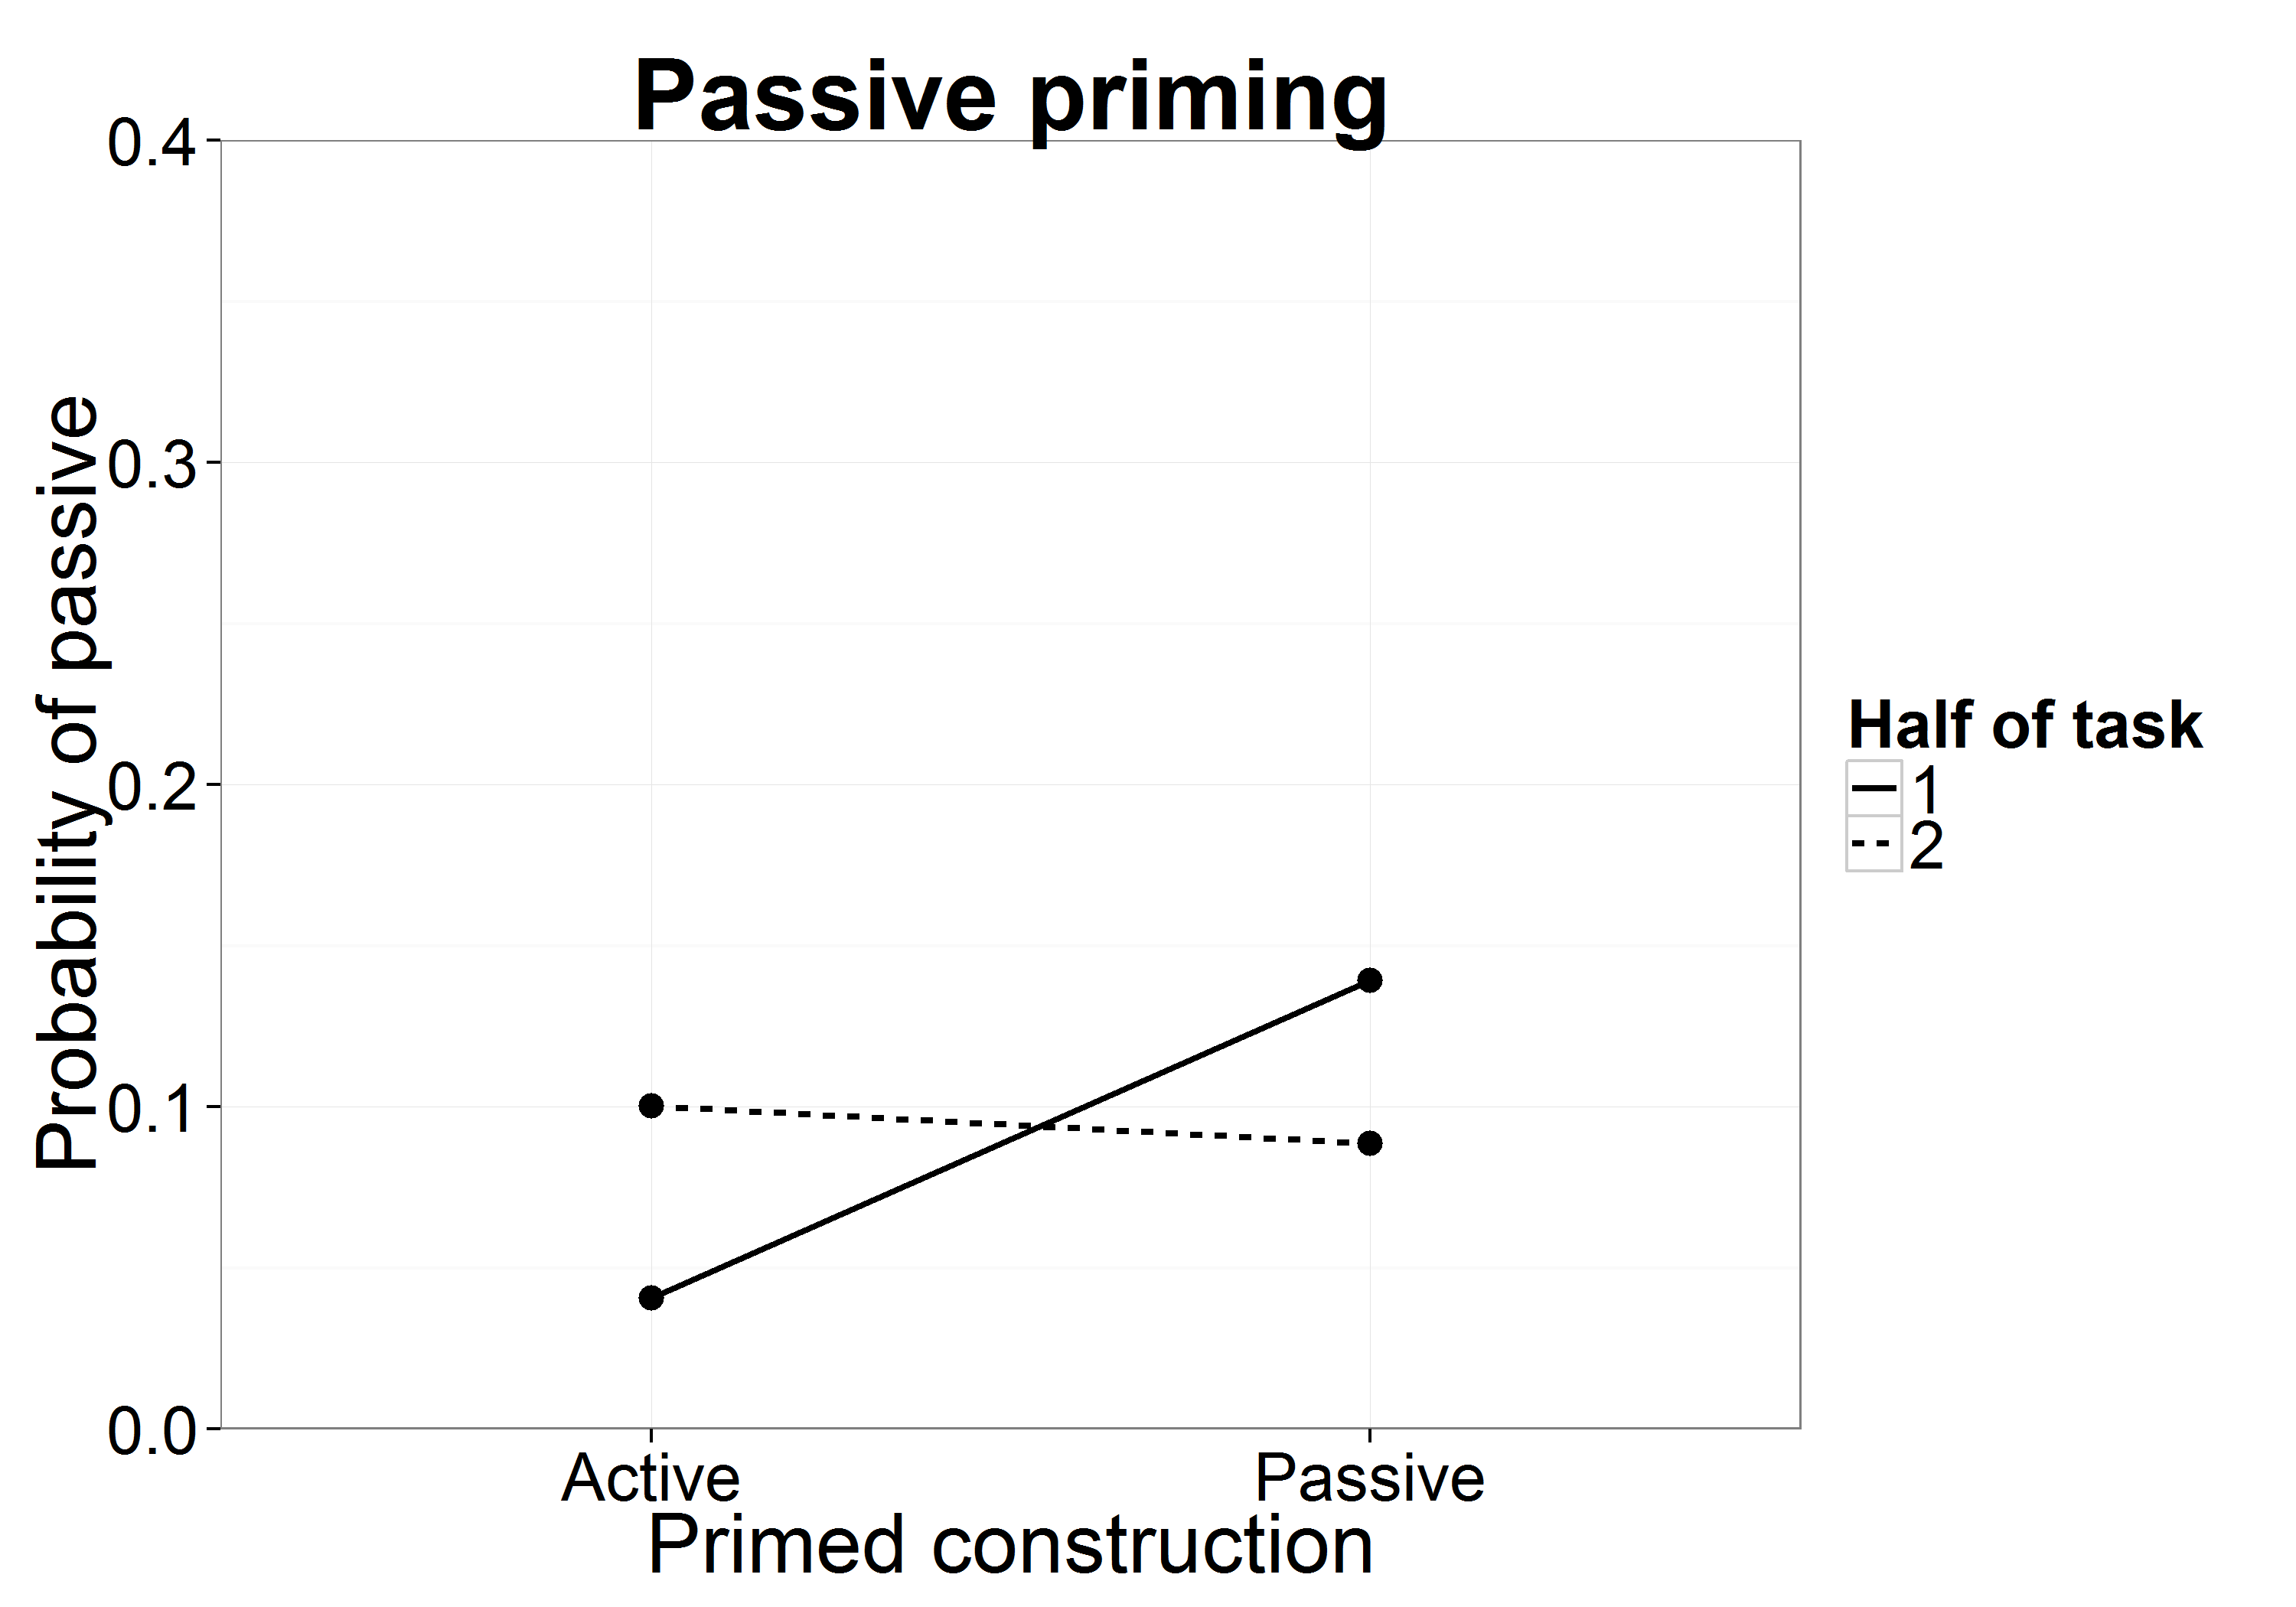
\includegraphics[width=\textwidth,height=\textheight,keepaspectratio]{ap.png}
\caption{Plotted model fits for the active and passive priming model.}
\label{fig:priming.fixef.ap}
\end{figure}



For a subset of the higher proficiency speakers, there was no effect of the block contrast. There was a significant effect of the contrast for primed structure (\emph{$\beta$} = --1.199, \emph{SE} = 0.513, \emph{z} = --2.337, \emph{p} $<$ 0.05). There was no interaction between the two contrasts (\emph{z} $<$ 1.96, \emph{p} $>$ 0.05).  See Table \ref{tab:priming.fixef.ap.hp} for the fixed-effects, and see Figure \ref{fig:priming.fixef.ap.hp} for a partial effects plot.

% Table generated by Excel2LaTeX from sheet 'Sheet23'
\begin{table}[htbp]
  \centering
  \caption{Fixed-effects model output for the active and passive conditions including only high-proficiency bilinguals.}
    \begin{tabular}{rrrrr}
    \toprule
          & Estimate & Std. Error & z value & Pr(>|z|) \\
    \midrule
    (Intercept) & -2.293 & 0.594 & -3.859 & 0 \\
    Block.desc1 & 0.035 & 0.504 & 0.069 & 0.945 \\
    Construction.ver1 & -1.199 & 0.513 & -2.337 & 0.019 \\
    Block.desc1:Construction.ver1 & -1.106 & 0.97  & -1.14 & 0.254 \\
    \bottomrule
    \end{tabular}%
  \label{tab:priming.fixef.ap.hp}%
\end{table}%

\begin{figure}[htbp]
\centering
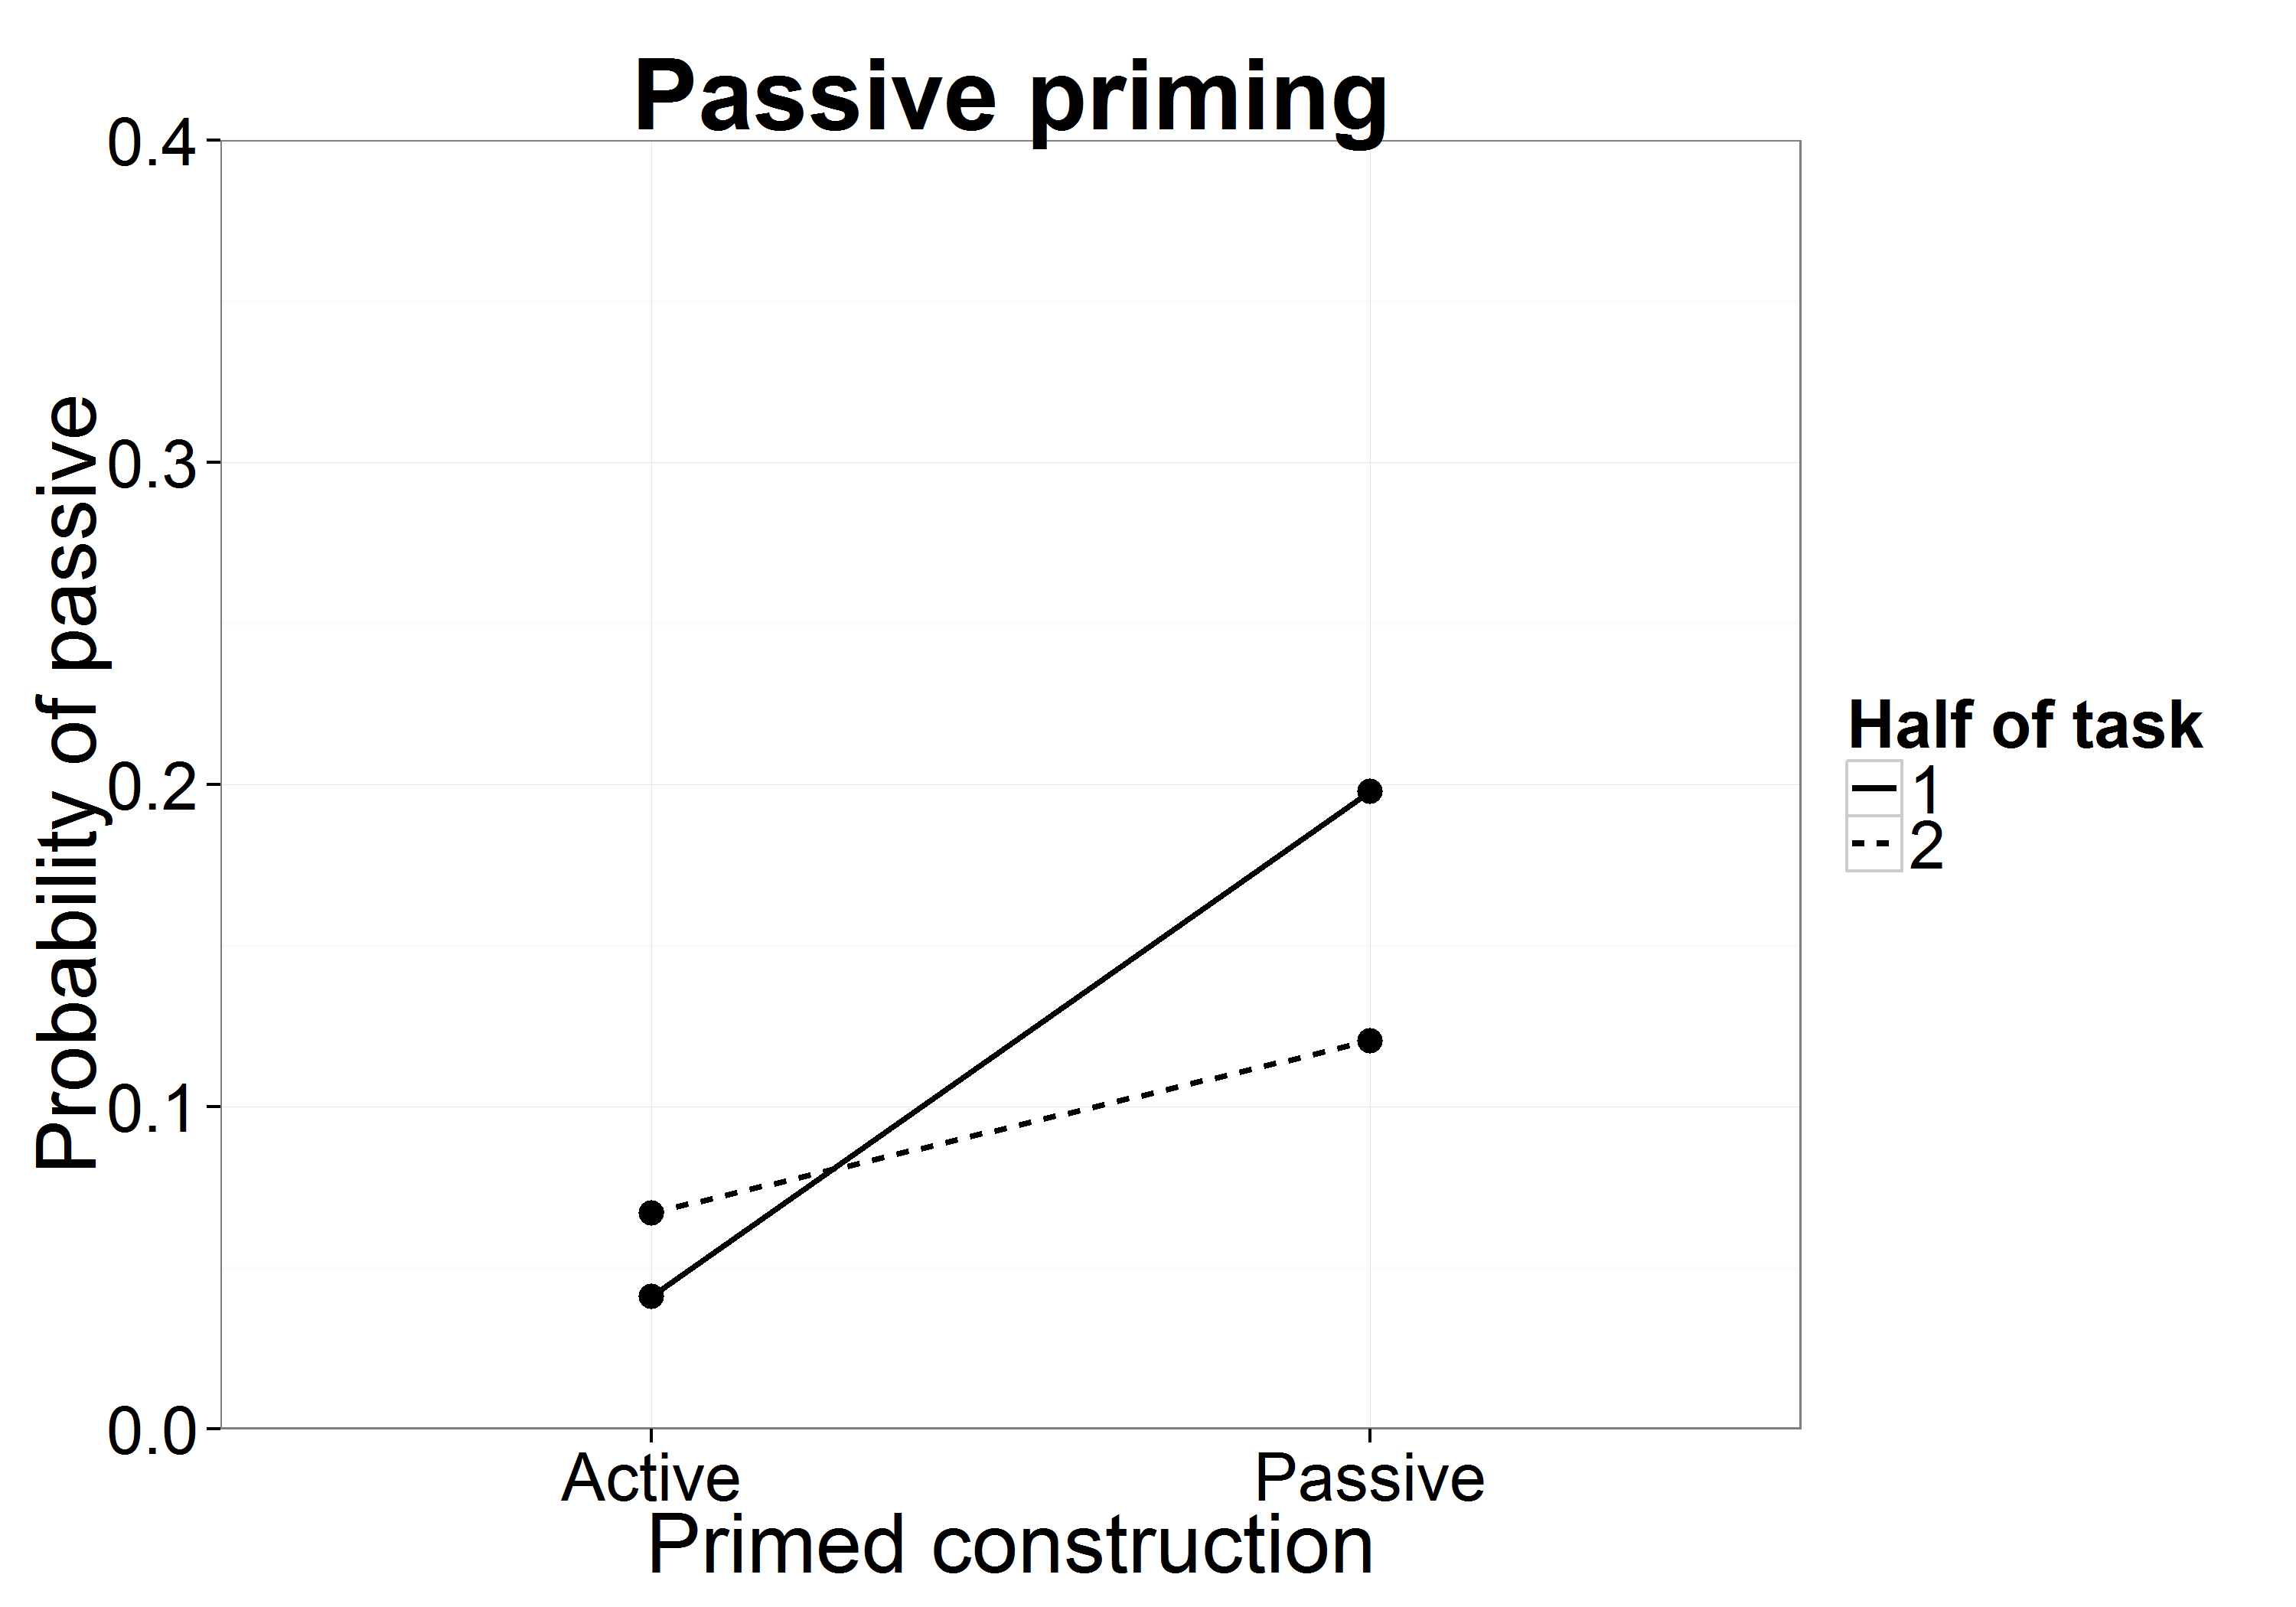
\includegraphics[width=\textwidth,height=\textheight,keepaspectratio]{ap_1.png}
\caption{Plotted model fits for the active and passive priming model including only high proficiency bilinguals.}
\label{fig:priming.fixef.ap.hp}
\end{figure}


For the dative conditions, neither the block contrast not the prime contrast were significant, nor was the interaction between the two contrasts (\emph{z}s $<$ 1, \emph{p}s $>$ 0.05). See Table \ref{tab:priming.fixef.dat} for the fixed-effects from the dative model, and see Figure \ref{fig:priming.fixef.dat} for a partial effects plot.

% Table generated by Excel2LaTeX from sheet 'Sheet24'
\begin{table}[htbp]
  \centering
  \caption{Fixed-effects model output for the dative conditions.}
    \begin{tabular}{rrrrr}
    \toprule
          & Estimate & Std. Error & z value & Pr(>|z|) \\
    \midrule
    (Intercept) & -2.847 & 0.355 & -8.017 & 0 \\
    Block.desc1 & -0.135 & 0.213 & -0.634 & 0.526 \\
    Construction.ver1 & -0.011 & 0.419 & -0.025 & 0.98 \\
    Block.desc1:Construction.ver1 & 0.342 & 0.429 & 0.799 & 0.425 \\
    \bottomrule
    \end{tabular}%
  \label{tab:priming.fixef.dat}%
\end{table}%

\begin{figure}[htbp]
\centering
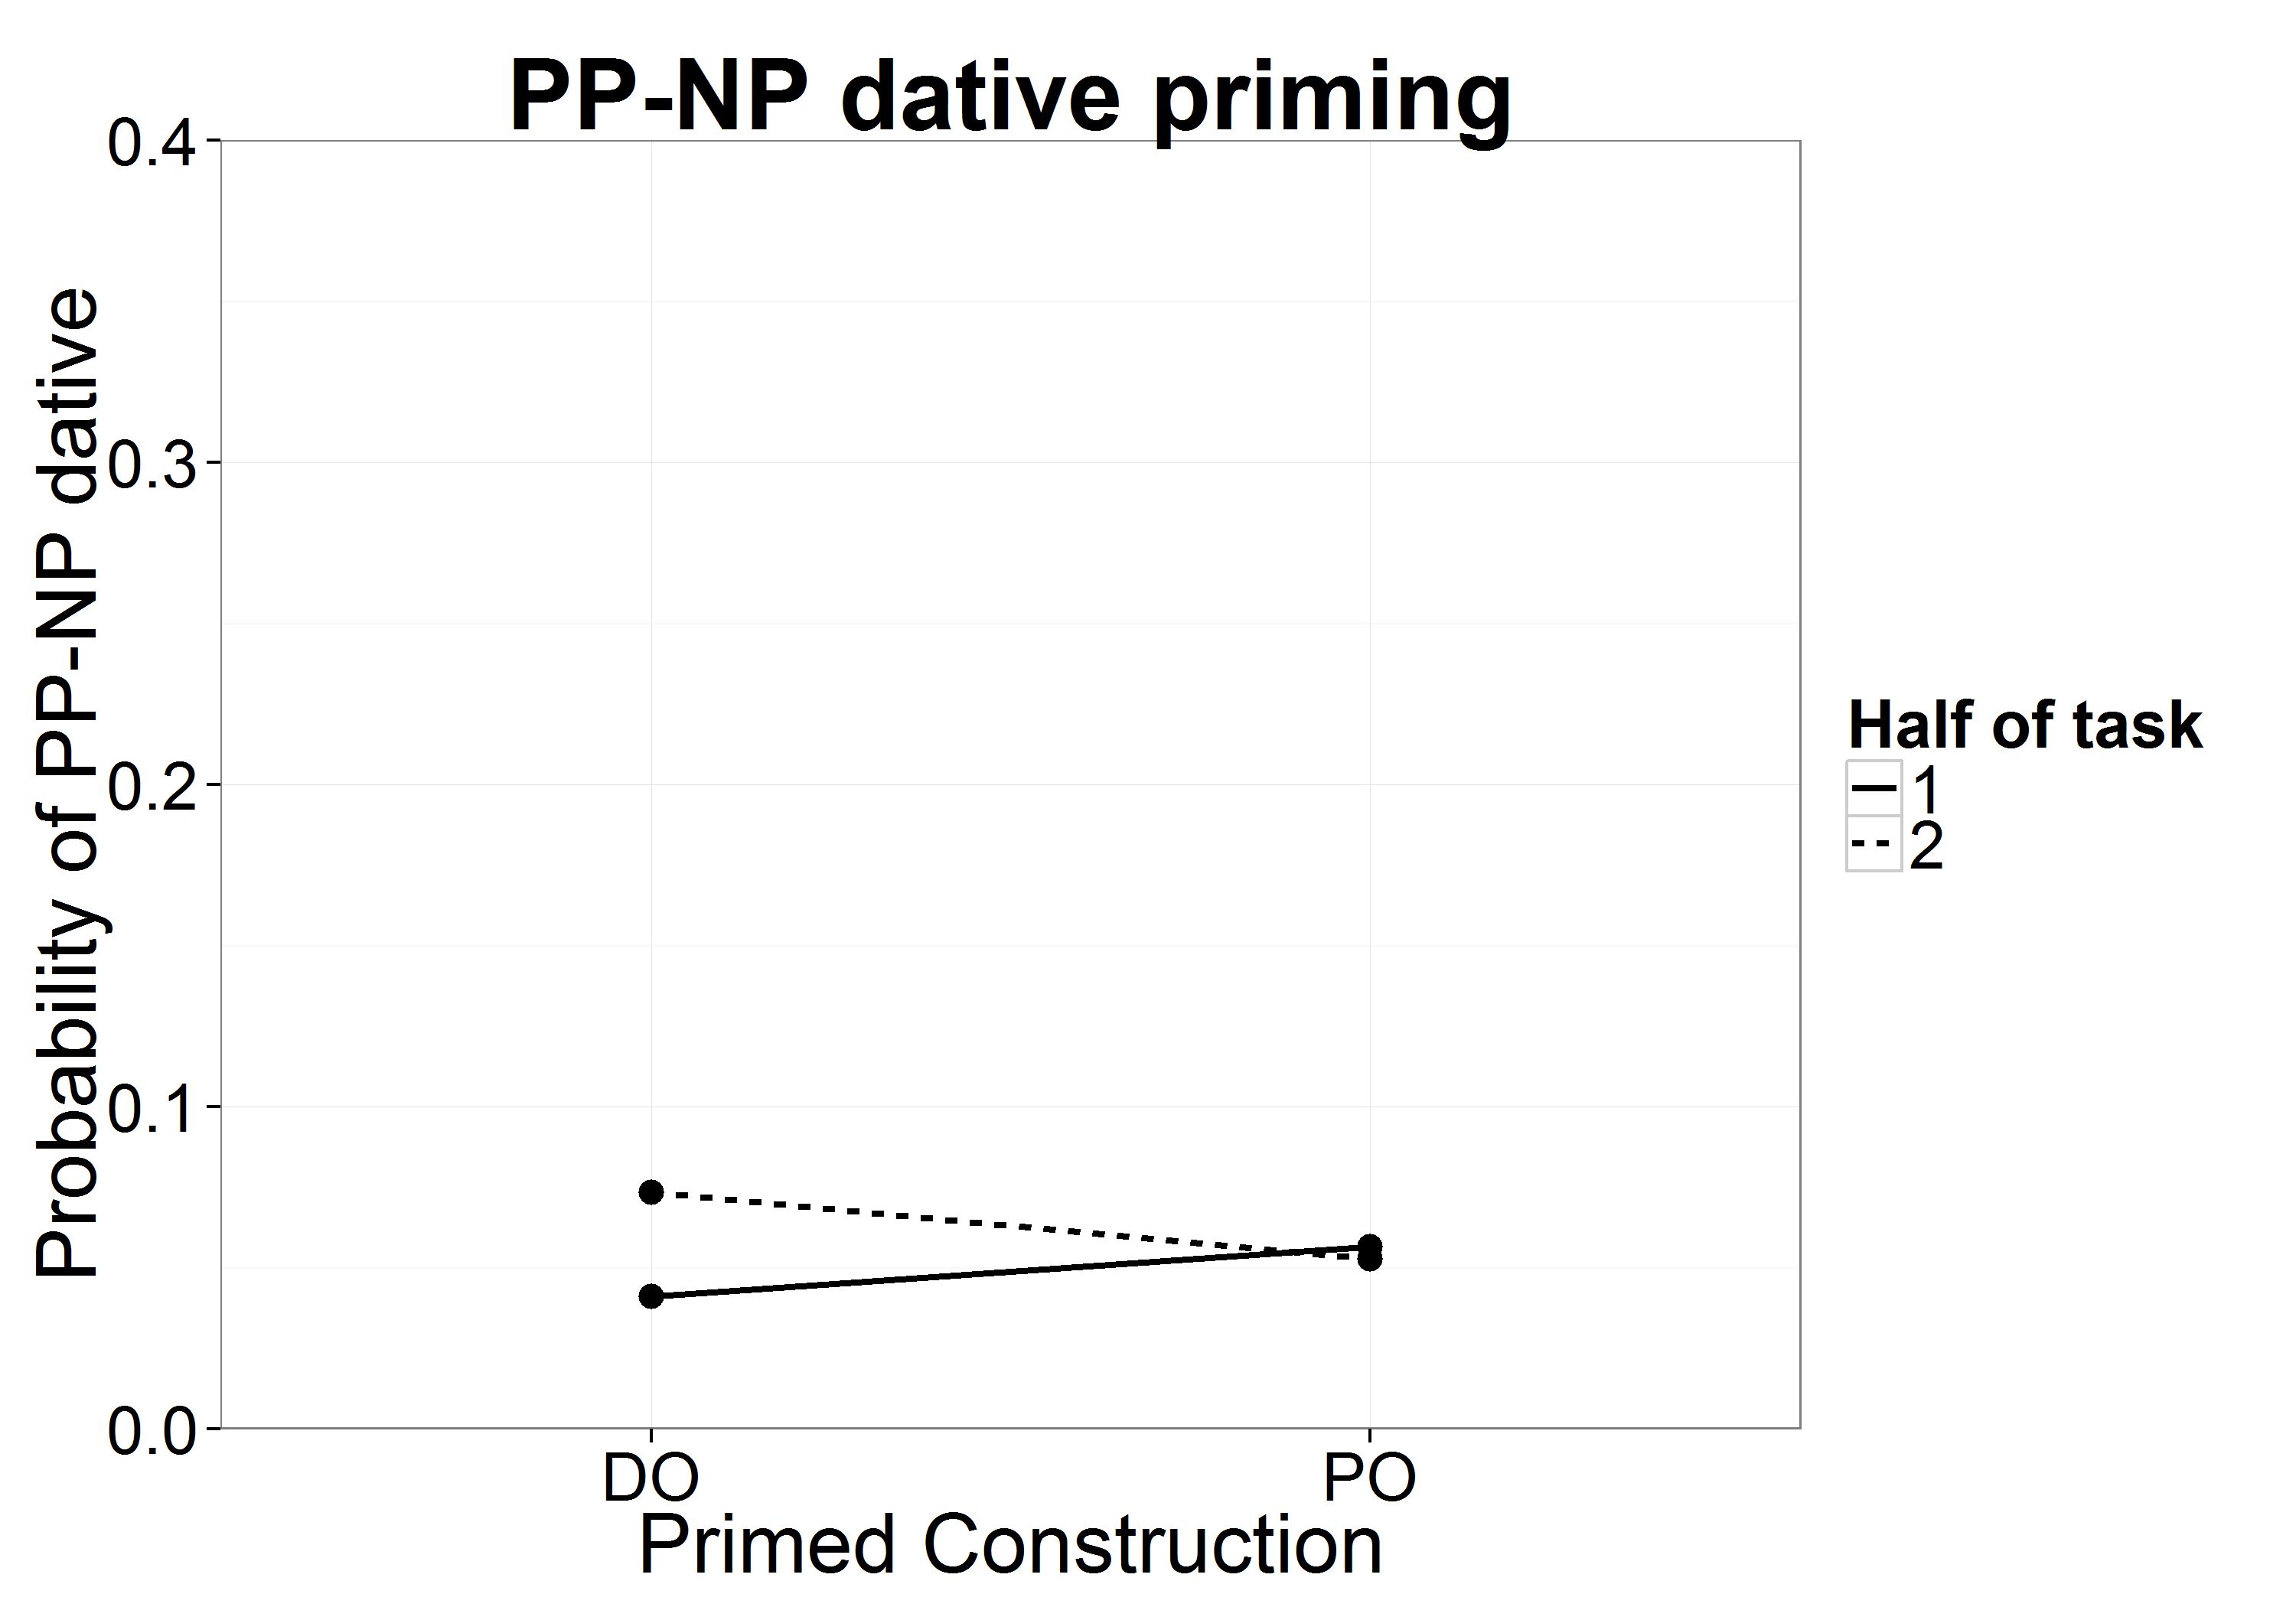
\includegraphics[width=\textwidth,height=\textheight,keepaspectratio]{dat.png}
\caption{Plotted model fits for the dative priming model. }
\label{fig:priming.fixef.dat}
\end{figure}


The subset of the higher proficiency speakers showed the same pattern of null results (\emph{z}s $<$ 1.96, \emph{p}s $>$ 0.05). The results were identical when we re-baselined to measure the likelihood of the participant producing a NP-PP dative after a NP-PP prime. See Table \ref{tab:priming.fixef.dat.hp} for the fixed-effects, and see Figure \ref{fig:priming.fixef.dat.hp} for a partial effects plot.

% Table generated by Excel2LaTeX from sheet 'Sheet25'
\begin{table}[htbp]
  \centering
  \caption{Fixed-effects model output for the dative conditions including only high proficiency bilinguals.}
    \begin{tabular}{rrrrr}
    \toprule
          & Estimate & Std. Error & z value & Pr(>|z|) \\
    \midrule
    (Intercept) & -3.138 & 0.509 & -6.164 & 0 \\
    Block.desc1 & -0.324 & 0.333 & -0.973 & 0.331 \\
    Construction.ver1 & 0.517 & 0.672 & 0.77  & 0.441 \\
    Block.desc1:Construction.ver1 & 0.973 & 0.669 & 1.453 & 0.146 \\
    \bottomrule
    \end{tabular}%
  \label{tab:priming.fixef.dat.hp}%
\end{table}%

\begin{figure}[htbp]
\centering
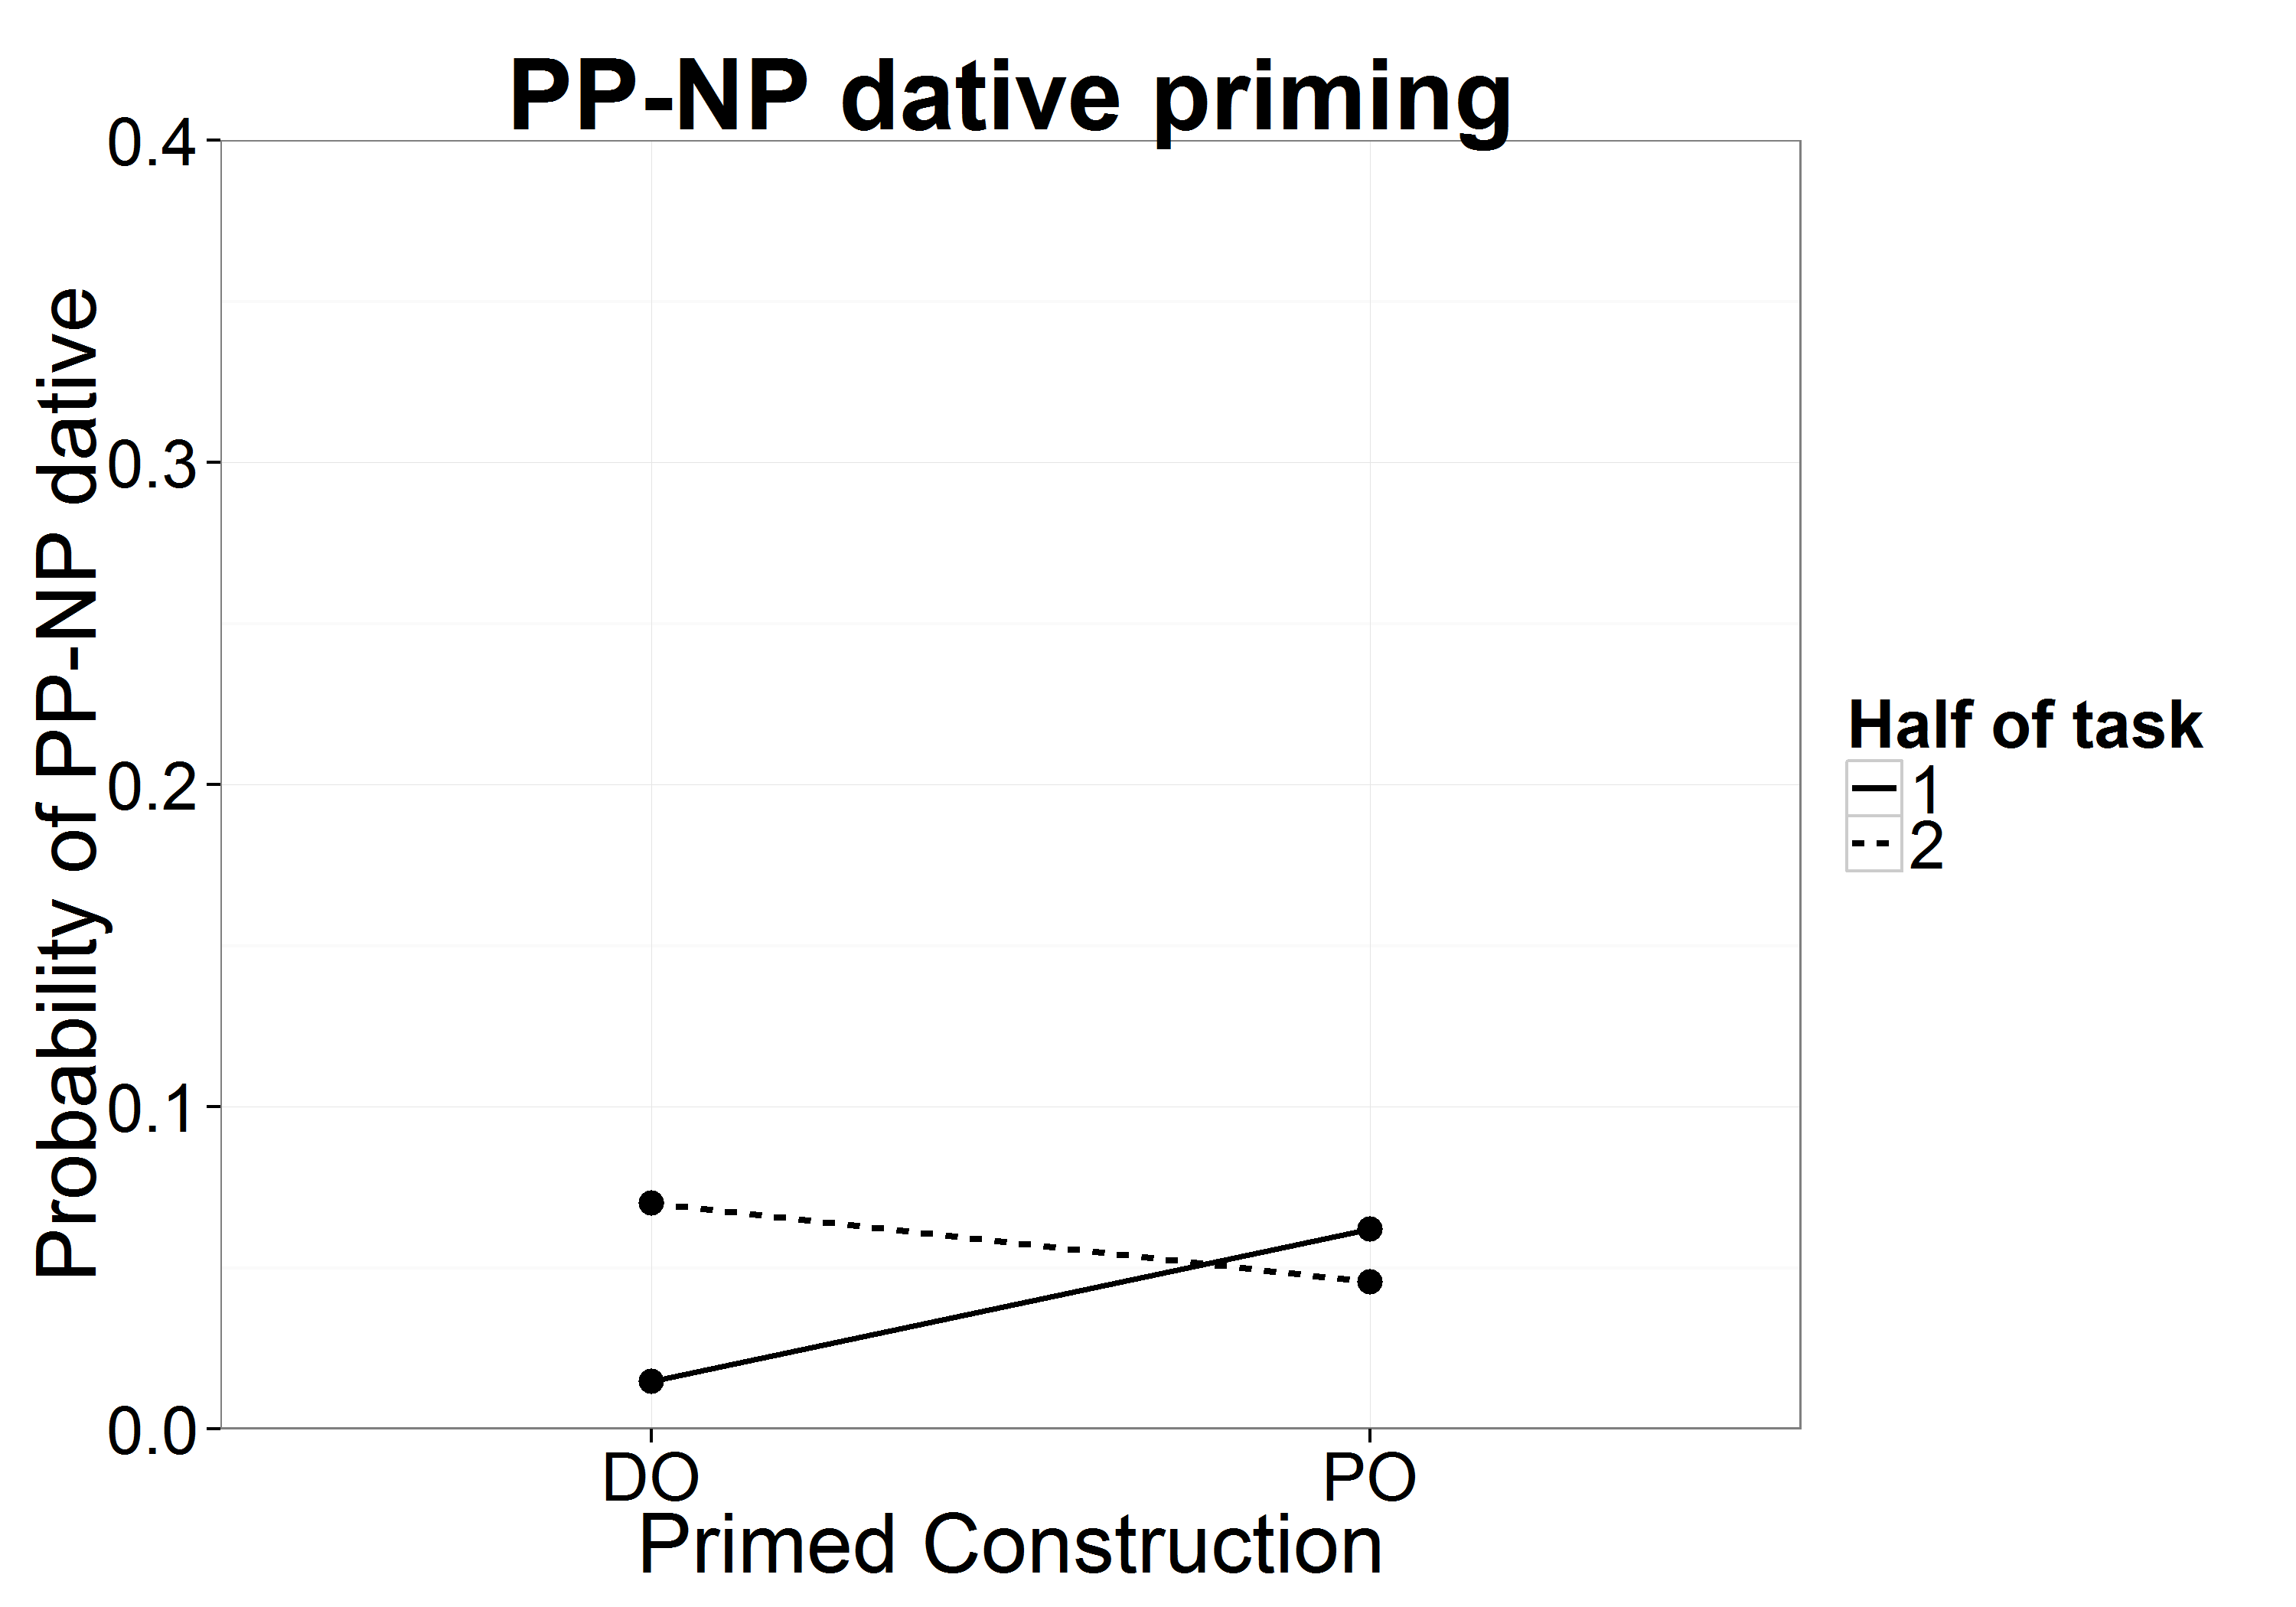
\includegraphics[width=\textwidth,height=\textheight,keepaspectratio]{dat_1.png}
\caption{Plotted model fits for the dative priming model including only high proficiency bilinguals. }
\label{fig:priming.fixef.dat.hp}
\end{figure}

\section{General Discussion}
\label{generaldiscussion}

We found evidence for shared structural representations in a sample of Spanish-English bilinguals. There was significant cross-language priming for the active and passive conditions: participants were more likely to produce a Spanish passive structure after they had just heard the confederate use an English passive structure. Crucially, the syntactic priming effect appeared to depend on shared linear order of arguments between English and Spanish. While active and passive sentences share word order between languages, prepositional object dative sentences do not. Spanish, but not English, contains a PP-NP prepositional object dative sentence (e.g., Un hombre mostrando a una mujer su celular [A man shows to a woman his phone]), and English, but not Spanish, contains a double object dative (e.g., The man shows his phone to the woman) without a prepositional object. In the dative conditions there was no hint of cross-language priming: participants did not produce more Spanish PP-NP datives after the confederate used an English double object dative, nor did the participant produce more Spanish NP-PP datives after the confederate produced English NP-PP datives. This suggests that datives may not have shared representations for our sample of Spanish-English bilinguals. 

Cross-language syntactic priming is in line with previous studies showing that bilinguals access syntactic representations that are not specified for language ~\citep[e.g.,][]{Loebell2003,Hartsuiker2004}. The present study extends these results in a few ways. First, this study demonstrates evidence for syntactic priming using a novel set of photographic description stimuli that has not been used in previous studies. Second, data from this experiment offer evidence for the implicit learning account of syntactic priming (this point is expanded below). Third, the present study serves as an important replication of the small number of reports on cross-language priming for Spanish-English bilinguals ~\citep{Flett2003,Hartsuiker2004,Meijer2003}. Finally, this study adds to a small, but growing, literature showing that bilinguals can have language-specific representations when structures do not share word order across two languages ~\citep{Bernolet2007, Loebell2003, Salamoura2007}.

\subsection{Novel stimuli}
\label{novelstimuli}

Many picture-description priming studies that investigate cross-language syntactic priming use a rigid set of stimuli. The prime structures are sometimes separated into between-participants experiments ~\citep[e.g.,][]{Bernolet2009}. The description pictures are commonly line drawings depicting agents, objects, and simple actions ~\citep[e.g.,][]{Bernolet2010,Flett2012,Hartsuiker2004,Loebell2003} and participants are often cued by the experimenter to use a particular verb ~\citep[e.g.,][]{Bernolet2010,Flett2012,Hartsuiker2004}. Given that cross-language syntactic priming is observed during naturalistic conversation, it seems important to extend the experimental results to a more naturalistic setting. In this study, we included both construction conditions (active\slash passive and dative) in one experiment, included photographic pictures of scenes or scenes digitally constructed from photographic objects, and we did not place restrictions on the verbs (and thus constructions) participants should use to describe our stimuli. Participants were therefore free to describe the picture using any construction they wanted and describe any aspect of the picture they felt was most salient in order to complete the task. While these decisions could potentially introduce unwanted variability into the stimuli, they also make for a more naturalistic task setting, allowing us to begin to bridge the gap between studies on priming in naturalistic conversation and priming in experimental settings. Under these conditions, we replicate the finding of cross-language syntactic priming between English and Spanish ~\citep{Flett2003, Hartsuiker2004, Meijer2003}, despite the potential variability introduced by the design decisions. Thus, our results suggest, along the lines of usage-based theories of language ~\citep{Bybee2006,Bybee2010}, that syntactic priming is a fundamental aspect of language processing. 

One potential consequence of our design choices is that we may have underestimated the cross-language syntactic priming effect through the introduction of additional variance in our experimental stimuli. On the one hand, this might mean that there could actually be syntactic priming, and hence a degree of shared representation, in the dative structures for our sample of bilinguals. However, on the other hand, there is no reason to assert that the increased variability would differentially affect the priming conditions (datives vs. active\slash passives). Therefore, we would still expect smaller priming effects in the dative sentences even in a perfectly controlled design, suggesting that the degree of shared representation for datives is less than that of actives and passives. 

\subsection{Implicit learning}
\label{implicitlearning}

Priming that is dependent on the time-course of the task is in line with an implicit learning account of syntactic priming ~\citep{Bock2000, Bock2007, Chang2006}. While we did not test for delayed priming, as is usual for implicit learning studies ~\citep[e.g.,][]{Bock2000}, we showed that the strength of passive priming was stronger at the beginning half of the task and decreased in the second block of the task via a significant prime by block interaction. This suggests that participants were tuning their mental representations to experience with the passive structure over the course of the task ~\citep{Chang2006}. There also appeared to be a hint that implicit learning depended on language proficiency. When we analyzed only high proficiency bilinguals, the interaction was no longer significant, and instead participants displayed uniform priming throughout the course of the task. The non-significant interaction could have resulted from a drop in statistical power (given the sample size was already small in the full analysis), or more speculatively, it could be indicative that higher and lower proficiency bilinguals tune their language systems to difference extents over the course of the task. Future research should investigate this issue further with larger samples of participants. 

\subsection{Extension of Spanish studies}
\label{extensionofspanishstudies}

The present study adds to the growing body of literature suggesting that bilingual speakers of Spanish and English have partially shared structural representations across the two languages. We found significant priming from English (L2) to Spanish (L1) in line with ~\citep{Meijer2003} for passive structures compared to active structures, in line with the results of  \citet{Hartsuiker2004} and  \citet{Flett2003}. Our results potentially conflict, however, with those of  \citet{Meijer2003}; they found significant priming between Spanish and English for propositional object dative structures, but we did not. This suggests that dative structures may actually share representations for Spanish and English despite the cross-language differences outlined in the Introduction. 

Our experiment differs from that of ~\citep{Meijer2003} in three ways. First, their study was a sentence recall task where ours was a picture description task. Perhaps different tasks are differentially sensitive to the cross-language syntactic priming. Second, the direction of priming differed between our two studies. While the sample of participants was very similar (Spanish-English bilinguals raised in the United States), the direction of priming was different between the two studies. They tested for priming from the L1 to the L2 (for the prepositional object structures) where we tested from L2 to L1. It is possible that production processes in the relatively weaker L2 are more likely piggyback structural representations from the L1 than vice versa. Thus while cross-language priming is weaker with lower proficiency bilinguals ~\citep{Bernolet2013}, there may be more complicated interactions between priming, proficiency, and the difficulty of the syntactic structure as operationalized by the existence of cross-language differences (e.g., in word order). This mirrors the emerging finding in the literature on bilingual lexical processing where researchers are finding complicated interactions between the degree of lexical co-activation, influences of sentence context, and proficiency ~\citep[e.g.,][, and see also the results from Chapter 4 of the present dissertation]{Pivneva2014}. Finally,  \citet{Meijer2003} only tested the NP-PP structure that overlapped in word order between the two languages. Specifically they found that participants can be primed to switch the word order of a memorized English double object dative to NP-PP dative after being presented with a Spanish NP-PP sentences (dative, locative, or instrumental primes). Crucially, there was no condition that tested a prime structure with non-overlapping word order, yet word order has been shown engender language-specific representations ~\citep[e.g.,][]{Bernolet2007}. 

\subsection{Language specific representations}
\label{languagespecificrepresentations}

Differential priming that is dependent on cross-language word order overlap is in line with previous studies showing that word order is a determinant in bilingual structural representation ~\citep{Bernolet2007,Loebell2003, Salamoura2007}. Previous studies have reported language-specific structural representations in German and English ~\citep{Bernolet2007, Loebell2003} and Greek and English ~\citep{Salamoura2007}. The present study is the first demonstration of language-specific structures for bilingual speakers of Spanish and English. Our bilingual sample showed significant cross-language priming in active and passive conditions, indicating that these structures share representational overlap between Spanish and English and that they are accessed in a manner that is non-specific to language during language production. In contrast, prepositional object conditions exhibited no hint of cross-language priming, suggesting that they are stored in language specific representational stores and are access in a language-specific manner. 

\section{Conclusion}
\label{conclusion}

In conclusion, we found that bilinguals have partially shared syntactic stores for their two linguistic systems. The sharedness appears to depend on word overlap between the two languages. When word order was shared, bilinguals exhibited significant cross-language syntactic priming consistent with an interpretation of shared structural representations. In contrast, when structures did not share word order there was no evidence for priming consistent with an interpretation of language-specific storage for the structures. This suggests that bilinguals attend to language specific cues that can drive the storage of linguistic units such as structural representations. 

%% \begin{landscape}
%% \section{Tables and Figures}
%% 



\clearpage




\clearpage




\clearpage





%% 

\clearpage


%% \end{landscape}



\chapter{General discussion and conclusions}
\label{generaldiscussionandconclusions}

The goal of this dissertation was to investigate how bilinguals select the language they intend to use at the lexical level and at the syntactic level. The hypothesis explored here is that cross-language differences in word order will allow bilinguals to predict the language of upcoming words in a sentence and to functionally separate syntactic structures. This hypothesis was addressed through the novel combination of two distinct research paradigms: the Rapid Serial Visual Presentation reading paradigm (RSVP; Chapter 4) and the confederate picture description task (Chapter 5). The RSVP allowed us to measure the co-activation of the two languages in a sample of Spanish-English bilinguals for words embedded in Spanish sentences. We manipulated the syntactic constructions used in the sentences such that some sentences contained word order overlap between English and Spanish (i.e., active, passive, and NP-PP dative sentences) and some contained no word order overlap (i.e., PP-NP dative sentences). Two norming studies (Chapter 3) confirmed that the lexical materials we selected to measure co-activation were as well matched as possible for lexical characteristics and did not show evidence for co-activation in a set of Spanish monolingual speakers. The picture description task allowed us to measure the degree of sharedness for the representation of syntactic structures in a sample of Spanish-English bilinguals. 

\section{Summary of results}
\label{summaryofresults}

\subsection{Summary of results from Chapter 3}
\label{summaryofresultsfromchapter3}

There were two goals of the pair of out-of-context word naming experiments in Chapter 3. The first goal was show that bilinguals access both languages non-selectively when words are presented in isolation and that monolinguals do not show similar effects. The second goal was to provide a baseline measure for the size of cognate and homograph effects for the sets of cognate and homograph as they are divided in study on naming words in sentence context. To this end, we conducted an out-of-context word naming experiment to measure on a group of Spanish monolinguals and Spanish-English bilinguals. 

The results of the two out-of context studies indicate that the selected cognate and homograph words were sufficient to elicit co-activation of English (the L2) when participants read words in Spanish (the L1). Co-activation was observable via significant cognate facilitation effect for the two sets of cognate stimuli, but not a homograph inhibition effect. Spanish monolinguals showed neither cognate effects no homograph effects when reading in Spanish, suggesting that the set of cognates was well-matched to the set of cognate-control items. Although from the monolingual results, the homographs appeared to be well controlled, there may have been lexical confounds present among the homograph stimuli that obscured a homograph inhibition effect. To account for this possibility, in Chapter 4, we conducted a reanalysis of the two norming studies and removed from both the out-of-context analysis as well as the in-context analysis any cognate items that did not show cognate facilitation and any homograph items that did not show homograph inhibition. Obviously, this resulted in significant effects for the out-of-context reanalysis, but we felt that it also strengthened the set of lexical stimuli for the analyses conducted in Chapter 4.

\subsection{Summary of results from Chapter 4}
\label{summaryofresultsfromchapter4}

The goal of the experiment in Chapter 4 was to combine observations from work on cross-language syntactic priming to identify a structure that should be considered language-specific between English and Spanish, and determine whether such a language-specific structure could allow Spanish-English bilinguals to selectively access the target language. The set of structures included actives, passives, and NP-PP datives (which all share word order and should share structural representation for Spanish and English) and PP-NP datives (which does not share word order between English and Spanish and should not share a structure representation). In the reading experiment, tested the degree of lexical co-activation under each of the sentence structures. 

We observed cognate (facilitation) and homograph (facilitation and inhibition) effects during the production of target words that were embedded in Spanish sentences. The magnitudes of the cognate and homograph effects relied on the syntactic structure of the sentence in which the targets were embedded. Cognate effects were significant in all sentences, but were greater for dative sentences that shared word order between English and Spanish in comparison to dative sentences that had word order differences between the two languages. The cognate modulation was weak, however; it depended on the set of items that were included in the analysis and was not significant when the set of items contained only those cognates and control pairs which demonstrated cognate facilitation in a separate out-of-context word naming task. In contrast, homograph effects robustly depended on the syntactic construction of the sentence, even when the subset of homograph-control pairs was restricted. Homograph effects were facilitatory in active and passive sentences, which contained word order overlap between English and Spanish. 

Furthermore, we found that cognate effects (but not homograph effects) depended on individual difference measures including fluency in the language of the task (Spanish, the L1), working memory span, and proactive inhibitory control. Cognate effects were generally smaller for individuals with greater pro-active control (i.e., those individuals who rely on contextual information) or for individuals with greater L1 fluency. 

\subsection{Summary of results from Chapter 5}
\label{summaryofresultsfromchapter5}

The goal of the present study was to determine the extent to which Spanish-English bilinguals share representations for syntactic structures using syntactic priming. The structures in question were actives, passives, NP-PP dative (which all share word order and should share structural representation for Spanish and English), and PP-NP dative sentences (which does not share word order between English and Spanish). 

We found evidence for shared structural representations that depended on word order overlap in a sample of Spanish-English bilinguals. There was significant cross-language priming for the active and passive conditions: participants were more likely to produce a Spanish passive structure after they had just heard the confederate use an English passive structure. In the dative conditions there was no hint of cross-language priming: participants did not produce more Spanish PP-NP datives after the confederate used an English double object dative, nor did the participant produce more Spanish NP-PP datives after the confederate produced English NP-PP datives.

\section{Conclusion}
\label{conclusion}

At the outset of this dissertation, we hypothesized that word order is crucially important in determining whether a syntactic structure is shared across the two languages or whether it must be accessed individually within each language, and that it is precisely this degree of language-specificity that might be utilized by bilinguals during word recognition as a cue, on top of the presence of a unilingual sentence context, to selectively activate the intended language. Overall, the results of this dissertation show that bilinguals share representations and co-activate both languages at both the lexical level and the syntactic level. Further, the results indicate that word order can function as cue to differentiate the two languages, reducing co-activation at each level. The results here also highlight the complicated nature of the interactions between language co-activation and other factors, including sentence context, executive function, and language proficiency. 

At the lexical level (Chapter 4), cognate effects and homograph effects were present when bilinguals read words in the context of sentences. This suggests that bilinguals co-activate lexical alternatives in both languages even when potentially useful context (e.g., a sentence context all in one language) is present that could in theory allow bilinguals to predict the language of upcoming words in the sentences ~\citep[e.g.,][]{Duyck2007}. Crucially, we showed for the first time that the magnitude of the cross-language effects depended on the syntactic construction of the sentence. Cognate facilitation was present in active and passive sentences, two structures that share word order between English and Spanish and have been shown to be language non-specific ~\citep{Hartsuiker2004} and in dative sentences, structures that exhibit differences in word order between English and Spanish and are hypothesized to be language-specific. However, the magnitude of cognate facilitation was marginally smaller for prepositional object dative sentences that did not share word order between English and Spanish. This suggests that the dative sentences (specifically the PP-NP sentences) may have triggered a language-specific response, reducing the magnitude of the cognate facilitation effect. Likewise, homograph effects were facilitatory in active and passive sentences (two structures that share word order between English and Spanish) but inhibitory in the two dative conditions, suggesting that the language specific information contained in the dative construction may have engendered a language-specific response observable via homograph inhibition. The cross-language effects for bilinguals do not appear to be driven by uncontrolled lexical properties between critical target words and controls, as monolinguals showed no such evidence of cognate facilitation or homograph inhibition (Chapter 3). Taken together, the lexical results suggest that syntax that is hypothesized to be language specific can influence the degree of lexical co-activation during sentence reading. 

In Chapter 5, we offer independent evidence for the role of word order in determining whether syntactic representations are shared across languages or stored in a language-specific manner. In the syntactic priming experiment, we observed significant priming in the active and passive condition where both structures share word order between the two languages, suggesting that active and passive have shared structural representations for our sample of Spanish-English bilinguals. In contrast there was no evidence of priming in dative conditions, suggesting that the two structures had distinct storage ~\citep[e.g.,][]{Bernolet2007,Loebell2003}. This greatly increases the strength of the claim that can be made regarding the role of word order overlap in modulating lexical co-activation at the lexical level.

The results reported here are in line with word recognition studies showing that a sentence context alone is not sufficient to eliminate co-activation of the unintended language, but that additional layers of context can modulate activation of the unintended language ~\citep[e.g.,][]{Schwartz2006,Libben2009}. The primary layer of context that has been shown to be significant in modulating co-activation of the unintended languages is a strongly biased semantic context. When the meaning of a sentence is highly predictable, it biases the reader to predict upcoming words in a sentence including, apparently, the language membership of that word ~\citep{Schwartz2006}. The results here extend these studies by showing that language-specific syntax can function in similar manner. Additionally, we show a modulating effect of cross-language activation without also speeding up the overall reaction time of recognition, eschewing the possibility that the magnitude change in cross-language effects is simply a side-effect of speeded recognition that masks a cross-language effect.

The evidence reported here that language-specific cues can reduce activation of the non-target language is in line with language-selective models of bilingual lexical access that assume bilinguals can use a selective attention mechanism perhaps guided by language-specific cues to alter the activation level of the non-target language ~\citep{Costa1999, Finkbeiner2006, LaHeij2005}. The syntactic context effects reported here are not explicitly predicted by the BIA+ model of word recognition. A strong version of the BIA+ model predicts that there should be no effects of linguistic context on word recognition. However, a weaker version predicts that any effects should occur late in processing. Future studies should investigate the time-course of these effects to validate or reject predictions made by BIA+.

Finally, more speculatively, the results from this dissertation are in line with an emerging literature showing that issues related to bilingual language co-activation and language control processes are not simple, main effects ~\citep[e.g.,][]{Bialystok2015,Green2013,Pivneva2014,Titone2011}. Instead they appear to depend on a complex interaction of internal and external influences. The observation of parallel language co-activation depends on multiple factors such as fluency in the L1, fluency in the L2, age of acquisition of the L2, and executive function ability, and the outcome of these interaction further influences the extent to which bilinguals can make use of contextual features of the input to modulate parallel activation ~\citep[e.g.,][; and the results reported here]{Pivneva2014,Titone2011}. Indeed, a recent proposal by ~\citep{Green2013} asserts the importance of the context of language usage in determining the exact type of cognitive control that bilinguals bring online to deal with cross-language co-activation. Thus, to greatly overgeneralize the research emerging in the last five years: bilingualism language control is complicated, and as researchers we should keep this finding in mind when interpreting the results of new studies. 

A hugely controversial literature exists surrounding a claim that bilinguals demonstrate superior general executive function compared to monolinguals due to increased language control demands. The original claim is that consistent application of executive control processes to manage multiple co-activated languages strengthens these processes, akin to exercising a muscle ~\citep{Bialystok2015,Paap2013}. However, the evidence for the bilingual advantage is not always consistent ~\citep{Costa2009,Paap2013}, and some have called into question the existence of the effect, arguing that the result is due to publication bias or invoking allusions to more nefarious methods of obtaining an effect ~\citep{deBruin2015,Paap2013,Paap2014}. Crucially, it is important consider that, perhaps, like bilingual language control, plasticity of executive function is complicated.


%%%%%%%%%%%%%%%%%%%%%%%%%%%%%%%%%%%%%%%%%%%%%%%%%%%%%%%%%%%%%%%
% Appendices
%
% Because of a quirk in LaTeX (see p. 48 of The LaTeX
% Companion, 2e), you cannot use \include along with
% \addtocontents if you want things to appear the proper
% sequence.
%%%%%%%%%%%%%%%%%%%%%%%%%%%%%%%%%%%%%%%%%%%%%%%%%%%%%%%%%%%%%%%
%% \appendix
%% \titleformat{\chapter}[display]{\fontsize{30}{30}\selectfont\bfseries\sffamily}{Appendix \thechapter\textcolor{gray75}{\raisebox{3pt}{|}}}{0pt}{}{}
%% % If you have a single appendix, then to prevent LaTeX from
%% % calling it ``Appendix A'', you should uncomment the following two
%% % lines that redefine the \thechapter and \thesection:
%% %\renewcommand\thechapter{}
%% %\renewcommand\thesection{\arabic{section}}
%% \Appendix{Out of context stimuli}\label{Appendix::Lexical}

%% \Appendix{Out of context stimuli}\label{Appendix::Sentential}


%%%%%%%%%%%%%%%%%%%%%%%%%%%%%%%%%%%%%%%%%%%%%%%%%%%%%%%%%%%%%%%
% ESM students need to include a Nontechnical Abstract as the %
% last appendix.                                              %
%%%%%%%%%%%%%%%%%%%%%%%%%%%%%%%%%%%%%%%%%%%%%%%%%%%%%%%%%%%%%%%
% This \include command should point to the file containing
% that abstract.
%\include{nontechnical-abstract}
%%%%%%%%%%%%%%%%%%%%%%%%%%%%%%%%%%%%%%%%%%%
} % End of the \allowdisplaybreak command %
%%%%%%%%%%%%%%%%%%%%%%%%%%%%%%%%%%%%%%%%%%%

%%%%%%%%%%%%%%%%
% BIBLIOGRAPHY %
%%%%%%%%%%%%%%%%
% You can use BibTeX or other bibliography facility for your
% bibliography. LaTeX's standard stuff is shown below. If you
% bibtex, then this section should look something like:
\addcontentsline{toc}{chapter}{Bibliography}
\printbibliography[notkeyword=noinclude]

%\begin{singlespace}
%\begin{thebibliography}{99}

%\frenchspacing

%\bibitem{Wisdom87} J. Wisdom, ``Rotational Dynamics of Irregularly Shaped Natural Satellites,'' \emph{The Astronomical Journal}, Vol.~94, No.~5, 1987  pp. 1350--1360.

%\bibitem{G&H83} J. Guckenheimer and P. Holmes, \emph{Nonlinear Oscillations, Dynamical Systems, and Bifurcations of Vector Fields}, Springer-Verlag, New York, 1983.

%\end{thebibliography}
%\end{singlespace}

\backmatter

% Vita
%\noindent
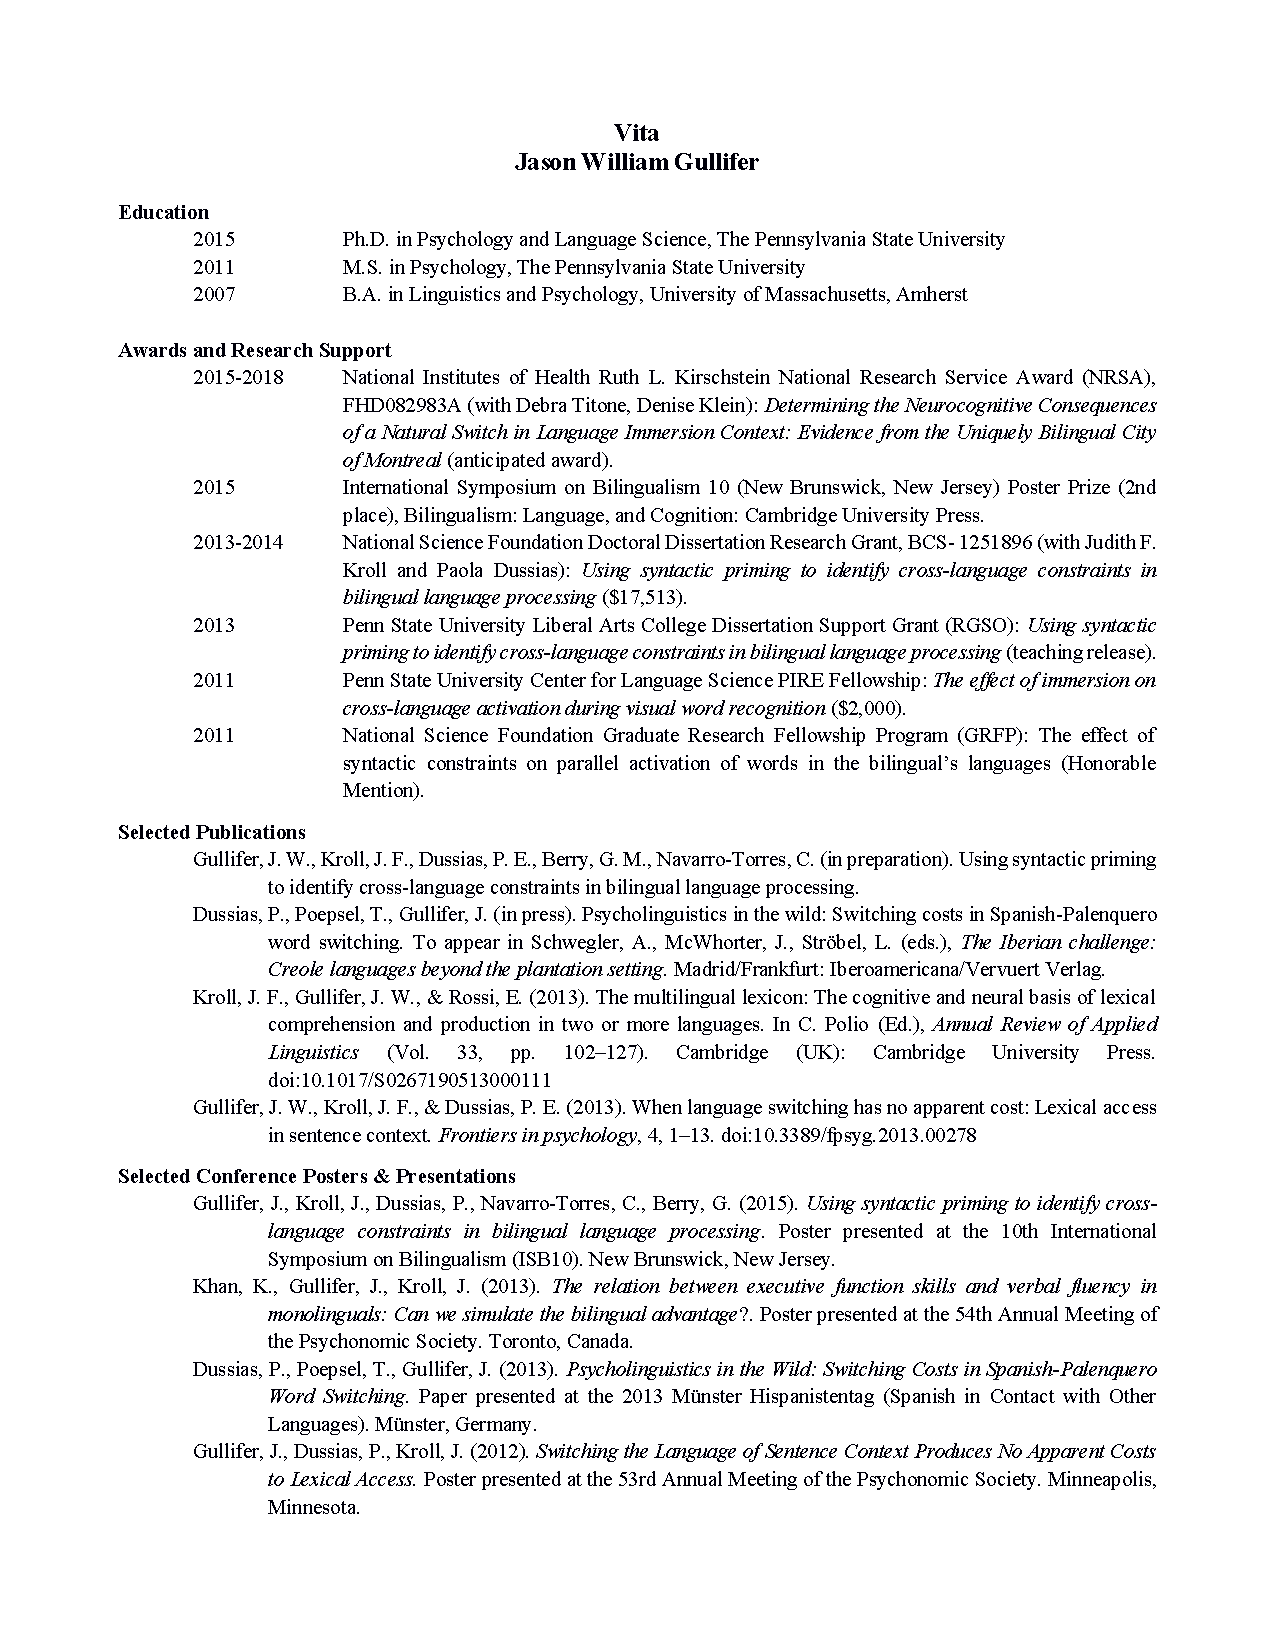
\includepdf[pages=-]{SupplementaryMaterial/vita.pdf}

\end{document}

